\documentclass[twoside]{book}

% Packages required by doxygen
\usepackage{fixltx2e}
\usepackage{calc}
\usepackage{doxygen}
\usepackage[export]{adjustbox} % also loads graphicx
\usepackage{graphicx}
\usepackage[utf8]{inputenc}
\usepackage{makeidx}
\usepackage{multicol}
\usepackage{multirow}
\PassOptionsToPackage{warn}{textcomp}
\usepackage{textcomp}
\usepackage[nointegrals]{wasysym}
\usepackage[table]{xcolor}

% Font selection
\usepackage[T1]{fontenc}
\usepackage[scaled=.90]{helvet}
\usepackage{courier}
\usepackage{amssymb}
\usepackage{sectsty}
\renewcommand{\familydefault}{\sfdefault}
\allsectionsfont{%
  \fontseries{bc}\selectfont%
  \color{darkgray}%
}
\renewcommand{\DoxyLabelFont}{%
  \fontseries{bc}\selectfont%
  \color{darkgray}%
}
\newcommand{\+}{\discretionary{\mbox{\scriptsize$\hookleftarrow$}}{}{}}

% Page & text layout
\usepackage{geometry}
\geometry{%
  a4paper,%
  top=2.5cm,%
  bottom=2.5cm,%
  left=2.5cm,%
  right=2.5cm%
}
\tolerance=750
\hfuzz=15pt
\hbadness=750
\setlength{\emergencystretch}{15pt}
\setlength{\parindent}{0cm}
\setlength{\parskip}{3ex plus 2ex minus 2ex}
\makeatletter
\renewcommand{\paragraph}{%
  \@startsection{paragraph}{4}{0ex}{-1.0ex}{1.0ex}{%
    \normalfont\normalsize\bfseries\SS@parafont%
  }%
}
\renewcommand{\subparagraph}{%
  \@startsection{subparagraph}{5}{0ex}{-1.0ex}{1.0ex}{%
    \normalfont\normalsize\bfseries\SS@subparafont%
  }%
}
\makeatother

% Headers & footers
\usepackage{fancyhdr}
\pagestyle{fancyplain}
\fancyhead[LE]{\fancyplain{}{\bfseries\thepage}}
\fancyhead[CE]{\fancyplain{}{}}
\fancyhead[RE]{\fancyplain{}{\bfseries\leftmark}}
\fancyhead[LO]{\fancyplain{}{\bfseries\rightmark}}
\fancyhead[CO]{\fancyplain{}{}}
\fancyhead[RO]{\fancyplain{}{\bfseries\thepage}}
\fancyfoot[LE]{\fancyplain{}{}}
\fancyfoot[CE]{\fancyplain{}{}}
\fancyfoot[RE]{\fancyplain{}{\bfseries\scriptsize Generated by Doxygen }}
\fancyfoot[LO]{\fancyplain{}{\bfseries\scriptsize Generated by Doxygen }}
\fancyfoot[CO]{\fancyplain{}{}}
\fancyfoot[RO]{\fancyplain{}{}}
\renewcommand{\footrulewidth}{0.4pt}
\renewcommand{\chaptermark}[1]{%
  \markboth{#1}{}%
}
\renewcommand{\sectionmark}[1]{%
  \markright{\thesection\ #1}%
}

% Indices & bibliography
\usepackage{natbib}
\usepackage[titles]{tocloft}
\setcounter{tocdepth}{3}
\setcounter{secnumdepth}{5}
\makeindex

% Hyperlinks (required, but should be loaded last)
\usepackage{ifpdf}
\ifpdf
  \usepackage[pdftex,pagebackref=true]{hyperref}
\else
  \usepackage[ps2pdf,pagebackref=true]{hyperref}
\fi
\hypersetup{%
  colorlinks=true,%
  linkcolor=blue,%
  citecolor=blue,%
  unicode%
}

% Custom commands
\newcommand{\clearemptydoublepage}{%
  \newpage{\pagestyle{empty}\cleardoublepage}%
}

\usepackage{caption}
\captionsetup{labelsep=space,justification=centering,font={bf},singlelinecheck=off,skip=4pt,position=top}

%===== C O N T E N T S =====

\begin{document}

% Titlepage & ToC
\hypersetup{pageanchor=false,
             bookmarksnumbered=true,
             pdfencoding=unicode
            }
\pagenumbering{alph}
\begin{titlepage}
\vspace*{7cm}
\begin{center}%
{\Large My Project }\\
\vspace*{1cm}
{\large Generated by Doxygen 1.8.14}\\
\end{center}
\end{titlepage}
\clearemptydoublepage
\pagenumbering{roman}
\tableofcontents
\clearemptydoublepage
\pagenumbering{arabic}
\hypersetup{pageanchor=true}

%--- Begin generated contents ---
\chapter{Hierarchical Index}
\section{Class Hierarchy}
This inheritance list is sorted roughly, but not completely, alphabetically\+:\begin{DoxyCompactList}
\item \contentsline{section}{Animate}{\pageref{class_animate}}{}
\item \contentsline{section}{Collision}{\pageref{class_collision}}{}
\item \contentsline{section}{Collision\+Handler}{\pageref{class_collision_handler}}{}
\item \contentsline{section}{Display}{\pageref{class_display}}{}
\item \contentsline{section}{Domain}{\pageref{class_domain}}{}
\item \contentsline{section}{File\+Not\+Found}{\pageref{class_file_not_found}}{}
\item \contentsline{section}{Game\+Files}{\pageref{class_game_files}}{}
\item \contentsline{section}{Game\+Loop}{\pageref{class_game_loop}}{}
\item \contentsline{section}{Game\+Object}{\pageref{class_game_object}}{}
\begin{DoxyCompactList}
\item \contentsline{section}{Centi\+Segment}{\pageref{class_centi_segment}}{}
\item \contentsline{section}{Lazer\+Shot}{\pageref{class_lazer_shot}}{}
\item \contentsline{section}{Mushroom}{\pageref{class_mushroom}}{}
\item \contentsline{section}{Scorpion}{\pageref{class_scorpion}}{}
\item \contentsline{section}{Spaceship}{\pageref{class_spaceship}}{}
\item \contentsline{section}{Spider}{\pageref{class_spider}}{}
\end{DoxyCompactList}
\item \contentsline{section}{Game\+Object\+Container}{\pageref{class_game_object_container}}{}
\begin{DoxyCompactList}
\item \contentsline{section}{Centipede}{\pageref{class_centipede}}{}
\item \contentsline{section}{Mushroom\+Field}{\pageref{class_mushroom_field}}{}
\end{DoxyCompactList}
\item \contentsline{section}{Non\+Movable\+Object}{\pageref{class_non_movable_object}}{}
\item \contentsline{section}{Object\+Out\+Of\+Bounds}{\pageref{class_object_out_of_bounds}}{}
\item \contentsline{section}{Player}{\pageref{class_player}}{}
\item \contentsline{section}{Score}{\pageref{class_score}}{}
\item \contentsline{section}{Splash\+Screen}{\pageref{class_splash_screen}}{}
\item \contentsline{section}{Timer}{\pageref{class_timer}}{}
\item \contentsline{section}{User\+Inputs}{\pageref{class_user_inputs}}{}
\item \contentsline{section}{vector2D}{\pageref{classvector2_d}}{}
\end{DoxyCompactList}

\chapter{Class Index}
\section{Class List}
Here are the classes, structs, unions and interfaces with brief descriptions\+:\begin{DoxyCompactList}
\item\contentsline{section}{\mbox{\hyperlink{class_animate}{Animate}} }{\pageref{class_animate}}{}
\item\contentsline{section}{\mbox{\hyperlink{class_centipede}{Centipede}} }{\pageref{class_centipede}}{}
\item\contentsline{section}{\mbox{\hyperlink{class_centi_segment}{Centi\+Segment}} }{\pageref{class_centi_segment}}{}
\item\contentsline{section}{\mbox{\hyperlink{class_collision}{Collision}} }{\pageref{class_collision}}{}
\item\contentsline{section}{\mbox{\hyperlink{class_collision_handler}{Collision\+Handler}} }{\pageref{class_collision_handler}}{}
\item\contentsline{section}{\mbox{\hyperlink{class_display}{Display}} }{\pageref{class_display}}{}
\item\contentsline{section}{\mbox{\hyperlink{class_domain}{Domain}} }{\pageref{class_domain}}{}
\item\contentsline{section}{\mbox{\hyperlink{class_file_not_found}{File\+Not\+Found}} }{\pageref{class_file_not_found}}{}
\item\contentsline{section}{\mbox{\hyperlink{class_game_files}{Game\+Files}} }{\pageref{class_game_files}}{}
\item\contentsline{section}{\mbox{\hyperlink{class_game_loop}{Game\+Loop}} }{\pageref{class_game_loop}}{}
\item\contentsline{section}{\mbox{\hyperlink{class_game_object}{Game\+Object}} }{\pageref{class_game_object}}{}
\item\contentsline{section}{\mbox{\hyperlink{class_game_object_container}{Game\+Object\+Container}} }{\pageref{class_game_object_container}}{}
\item\contentsline{section}{\mbox{\hyperlink{class_lazer_shot}{Lazer\+Shot}} }{\pageref{class_lazer_shot}}{}
\item\contentsline{section}{\mbox{\hyperlink{class_mushroom}{Mushroom}} }{\pageref{class_mushroom}}{}
\item\contentsline{section}{\mbox{\hyperlink{class_mushroom_field}{Mushroom\+Field}} }{\pageref{class_mushroom_field}}{}
\item\contentsline{section}{\mbox{\hyperlink{class_non_movable_object}{Non\+Movable\+Object}} }{\pageref{class_non_movable_object}}{}
\item\contentsline{section}{\mbox{\hyperlink{class_object_out_of_bounds}{Object\+Out\+Of\+Bounds}} }{\pageref{class_object_out_of_bounds}}{}
\item\contentsline{section}{\mbox{\hyperlink{class_player}{Player}} }{\pageref{class_player}}{}
\item\contentsline{section}{\mbox{\hyperlink{class_score}{Score}} }{\pageref{class_score}}{}
\item\contentsline{section}{\mbox{\hyperlink{class_scorpion}{Scorpion}} }{\pageref{class_scorpion}}{}
\item\contentsline{section}{\mbox{\hyperlink{class_spaceship}{Spaceship}} }{\pageref{class_spaceship}}{}
\item\contentsline{section}{\mbox{\hyperlink{class_spider}{Spider}} }{\pageref{class_spider}}{}
\item\contentsline{section}{\mbox{\hyperlink{class_splash_screen}{Splash\+Screen}} }{\pageref{class_splash_screen}}{}
\item\contentsline{section}{\mbox{\hyperlink{class_timer}{Timer}} }{\pageref{class_timer}}{}
\item\contentsline{section}{\mbox{\hyperlink{class_user_inputs}{User\+Inputs}} }{\pageref{class_user_inputs}}{}
\item\contentsline{section}{\mbox{\hyperlink{classvector2_d}{vector2D}} }{\pageref{classvector2_d}}{}
\end{DoxyCompactList}

\chapter{File Index}
\section{File List}
Here is a list of all documented files with brief descriptions\+:\begin{DoxyCompactList}
\item\contentsline{section}{C\+:/\+Users/bvrad/\+Dropbox/\+Boikanyo/elen3009/\+P\+R\+O\+J\+E\+C\+T/2018-\/project-\/1386807-\/\+Radiokana-\/1427726-\/\+Sepuru/game-\/source-\/code/\mbox{\hyperlink{_animate_8h}{Animate.\+h}} \\*This class is used to draw all game entities onto the screen }{\pageref{_animate_8h}}{}
\item\contentsline{section}{C\+:/\+Users/bvrad/\+Dropbox/\+Boikanyo/elen3009/\+P\+R\+O\+J\+E\+C\+T/2018-\/project-\/1386807-\/\+Radiokana-\/1427726-\/\+Sepuru/game-\/source-\/code/\mbox{\hyperlink{_centipede_8h}{Centipede.\+h}} \\*This class inherits from \mbox{\hyperlink{class_game_object_container}{Game\+Object\+Container}}, the class forms a collection of Centi\+Segments that together make a \mbox{\hyperlink{class_centipede}{Centipede}} }{\pageref{_centipede_8h}}{}
\item\contentsline{section}{C\+:/\+Users/bvrad/\+Dropbox/\+Boikanyo/elen3009/\+P\+R\+O\+J\+E\+C\+T/2018-\/project-\/1386807-\/\+Radiokana-\/1427726-\/\+Sepuru/game-\/source-\/code/\mbox{\hyperlink{_collision_8h}{Collision.\+h}} \\*This class checks for collision between two Game\+Objects }{\pageref{_collision_8h}}{}
\item\contentsline{section}{C\+:/\+Users/bvrad/\+Dropbox/\+Boikanyo/elen3009/\+P\+R\+O\+J\+E\+C\+T/2018-\/project-\/1386807-\/\+Radiokana-\/1427726-\/\+Sepuru/game-\/source-\/code/\mbox{\hyperlink{_collision_handler_8h}{Collision\+Handler.\+h}} \\*This class handles collison of Game\+Objects }{\pageref{_collision_handler_8h}}{}
\item\contentsline{section}{C\+:/\+Users/bvrad/\+Dropbox/\+Boikanyo/elen3009/\+P\+R\+O\+J\+E\+C\+T/2018-\/project-\/1386807-\/\+Radiokana-\/1427726-\/\+Sepuru/game-\/source-\/code/\mbox{\hyperlink{_constants_8h}{Constants.\+h}} \\*The file contains all constanst used in the Game }{\pageref{_constants_8h}}{}
\item\contentsline{section}{C\+:/\+Users/bvrad/\+Dropbox/\+Boikanyo/elen3009/\+P\+R\+O\+J\+E\+C\+T/2018-\/project-\/1386807-\/\+Radiokana-\/1427726-\/\+Sepuru/game-\/source-\/code/\mbox{\hyperlink{_csegment_8h}{Csegment.\+h}} \\*This class models the attributes and behaviour of a segment of a Centiped. The Class inherits \mbox{\hyperlink{class_game_object}{Game\+Object}} }{\pageref{_csegment_8h}}{}
\item\contentsline{section}{C\+:/\+Users/bvrad/\+Dropbox/\+Boikanyo/elen3009/\+P\+R\+O\+J\+E\+C\+T/2018-\/project-\/1386807-\/\+Radiokana-\/1427726-\/\+Sepuru/game-\/source-\/code/\mbox{\hyperlink{_display_8h}{Display.\+h}} \\*Renders the \mbox{\hyperlink{class_game_object}{Game\+Object}} onto the screen }{\pageref{_display_8h}}{}
\item\contentsline{section}{C\+:/\+Users/bvrad/\+Dropbox/\+Boikanyo/elen3009/\+P\+R\+O\+J\+E\+C\+T/2018-\/project-\/1386807-\/\+Radiokana-\/1427726-\/\+Sepuru/game-\/source-\/code/\mbox{\hyperlink{_domain_8h}{Domain.\+h}} \\*This class is where all the Logic objects interact }{\pageref{_domain_8h}}{}
\item\contentsline{section}{C\+:/\+Users/bvrad/\+Dropbox/\+Boikanyo/elen3009/\+P\+R\+O\+J\+E\+C\+T/2018-\/project-\/1386807-\/\+Radiokana-\/1427726-\/\+Sepuru/game-\/source-\/code/\mbox{\hyperlink{_game_files_8h}{Game\+Files.\+h}} \\*Database for all the game\textquotesingle{}s classes }{\pageref{_game_files_8h}}{}
\item\contentsline{section}{C\+:/\+Users/bvrad/\+Dropbox/\+Boikanyo/elen3009/\+P\+R\+O\+J\+E\+C\+T/2018-\/project-\/1386807-\/\+Radiokana-\/1427726-\/\+Sepuru/game-\/source-\/code/\mbox{\hyperlink{_game_loop_8h}{Game\+Loop.\+h}} \\*This class is the main controller of the Game, it is the Game Engine }{\pageref{_game_loop_8h}}{}
\item\contentsline{section}{C\+:/\+Users/bvrad/\+Dropbox/\+Boikanyo/elen3009/\+P\+R\+O\+J\+E\+C\+T/2018-\/project-\/1386807-\/\+Radiokana-\/1427726-\/\+Sepuru/game-\/source-\/code/\mbox{\hyperlink{_game_object_8h}{Game\+Object.\+h}} \\*This is the parent to all of the game\+Object, it models an entity in a 2D space }{\pageref{_game_object_8h}}{}
\item\contentsline{section}{C\+:/\+Users/bvrad/\+Dropbox/\+Boikanyo/elen3009/\+P\+R\+O\+J\+E\+C\+T/2018-\/project-\/1386807-\/\+Radiokana-\/1427726-\/\+Sepuru/game-\/source-\/code/\mbox{\hyperlink{_game_object_container_8h}{Game\+Object\+Container.\+h}} \\*This class is a blue print to containers of type Game\+Objects }{\pageref{_game_object_container_8h}}{}
\item\contentsline{section}{C\+:/\+Users/bvrad/\+Dropbox/\+Boikanyo/elen3009/\+P\+R\+O\+J\+E\+C\+T/2018-\/project-\/1386807-\/\+Radiokana-\/1427726-\/\+Sepuru/game-\/source-\/code/\mbox{\hyperlink{_game_types_8h}{Game\+Types.\+h}} \\*This vector mimics a 2D vector that takes in an x and y value for representation of game objects in a 2D space }{\pageref{_game_types_8h}}{}
\item\contentsline{section}{C\+:/\+Users/bvrad/\+Dropbox/\+Boikanyo/elen3009/\+P\+R\+O\+J\+E\+C\+T/2018-\/project-\/1386807-\/\+Radiokana-\/1427726-\/\+Sepuru/game-\/source-\/code/\mbox{\hyperlink{_lazer_shot_8h}{Lazer\+Shot.\+h}} \\*Derived from \mbox{\hyperlink{class_game_object}{Game\+Object}} class, it models a \mbox{\hyperlink{class_lazer_shot}{Lazer\+Shot}} in the Game space }{\pageref{_lazer_shot_8h}}{}
\item\contentsline{section}{C\+:/\+Users/bvrad/\+Dropbox/\+Boikanyo/elen3009/\+P\+R\+O\+J\+E\+C\+T/2018-\/project-\/1386807-\/\+Radiokana-\/1427726-\/\+Sepuru/game-\/source-\/code/\mbox{\hyperlink{_mushroom_8h}{Mushroom.\+h}} \\*Derived from \mbox{\hyperlink{class_game_object}{Game\+Object}}, the class models the representation of a \mbox{\hyperlink{class_mushroom}{Mushroom}} object in the Game Space }{\pageref{_mushroom_8h}}{}
\item\contentsline{section}{C\+:/\+Users/bvrad/\+Dropbox/\+Boikanyo/elen3009/\+P\+R\+O\+J\+E\+C\+T/2018-\/project-\/1386807-\/\+Radiokana-\/1427726-\/\+Sepuru/game-\/source-\/code/\mbox{\hyperlink{_mushroom_field_8h}{Mushroom\+Field.\+h}} \\*This class is responsible for randomly generating a field Mushrooms on Game Play }{\pageref{_mushroom_field_8h}}{}
\item\contentsline{section}{C\+:/\+Users/bvrad/\+Dropbox/\+Boikanyo/elen3009/\+P\+R\+O\+J\+E\+C\+T/2018-\/project-\/1386807-\/\+Radiokana-\/1427726-\/\+Sepuru/game-\/source-\/code/\mbox{\hyperlink{_player_8h}{Player.\+h}} \\*This class is responsible for controlling the \mbox{\hyperlink{class_player}{Player}} }{\pageref{_player_8h}}{}
\item\contentsline{section}{C\+:/\+Users/bvrad/\+Dropbox/\+Boikanyo/elen3009/\+P\+R\+O\+J\+E\+C\+T/2018-\/project-\/1386807-\/\+Radiokana-\/1427726-\/\+Sepuru/game-\/source-\/code/\mbox{\hyperlink{_score_8h}{Score.\+h}} \\*This class is responsible keeping score }{\pageref{_score_8h}}{}
\item\contentsline{section}{C\+:/\+Users/bvrad/\+Dropbox/\+Boikanyo/elen3009/\+P\+R\+O\+J\+E\+C\+T/2018-\/project-\/1386807-\/\+Radiokana-\/1427726-\/\+Sepuru/game-\/source-\/code/\mbox{\hyperlink{_scorpion_8h}{Scorpion.\+h}} \\*Derived from \mbox{\hyperlink{class_game_object}{Game\+Object}} class, the \mbox{\hyperlink{class_scorpion}{Scorpion}} class models the representation of a \mbox{\hyperlink{class_scorpion}{Scorpion}} in 2D }{\pageref{_scorpion_8h}}{}
\item\contentsline{section}{C\+:/\+Users/bvrad/\+Dropbox/\+Boikanyo/elen3009/\+P\+R\+O\+J\+E\+C\+T/2018-\/project-\/1386807-\/\+Radiokana-\/1427726-\/\+Sepuru/game-\/source-\/code/\mbox{\hyperlink{_spaceship_8h}{Spaceship.\+h}} \\*This class is derived from the \mbox{\hyperlink{class_game_object}{Game\+Object}} class and models the \mbox{\hyperlink{class_spaceship}{Spaceship}} in a 2D space }{\pageref{_spaceship_8h}}{}
\item\contentsline{section}{C\+:/\+Users/bvrad/\+Dropbox/\+Boikanyo/elen3009/\+P\+R\+O\+J\+E\+C\+T/2018-\/project-\/1386807-\/\+Radiokana-\/1427726-\/\+Sepuru/game-\/source-\/code/\mbox{\hyperlink{_spider_8h}{Spider.\+h}} \\*Derived from \mbox{\hyperlink{class_game_object}{Game\+Object}} class, the models a \mbox{\hyperlink{class_spider}{Spider}} in 2D }{\pageref{_spider_8h}}{}
\item\contentsline{section}{C\+:/\+Users/bvrad/\+Dropbox/\+Boikanyo/elen3009/\+P\+R\+O\+J\+E\+C\+T/2018-\/project-\/1386807-\/\+Radiokana-\/1427726-\/\+Sepuru/game-\/source-\/code/\mbox{\hyperlink{_splash_screen_8h}{Splash\+Screen.\+h}} \\*This class presents the user\+Interface of the Game }{\pageref{_splash_screen_8h}}{}
\item\contentsline{section}{C\+:/\+Users/bvrad/\+Dropbox/\+Boikanyo/elen3009/\+P\+R\+O\+J\+E\+C\+T/2018-\/project-\/1386807-\/\+Radiokana-\/1427726-\/\+Sepuru/game-\/source-\/code/\mbox{\hyperlink{_timer_8h}{Timer.\+h}} \\*Responsible for timing Game\+Objects }{\pageref{_timer_8h}}{}
\item\contentsline{section}{C\+:/\+Users/bvrad/\+Dropbox/\+Boikanyo/elen3009/\+P\+R\+O\+J\+E\+C\+T/2018-\/project-\/1386807-\/\+Radiokana-\/1427726-\/\+Sepuru/game-\/source-\/code/\mbox{\hyperlink{_user_inputs_8h}{User\+Inputs.\+h}} \\*Responsible for Handling user inputs }{\pageref{_user_inputs_8h}}{}
\end{DoxyCompactList}

\chapter{Class Documentation}
\hypertarget{class_animate}{}\section{Animate Class Reference}
\label{class_animate}\index{Animate@{Animate}}


{\ttfamily \#include $<$Animate.\+h$>$}

\subsection*{Public Member Functions}
\begin{DoxyCompactItemize}
\item 
\mbox{\hyperlink{class_animate_ac76ff6cc4d70ec93f9b93ccc5c843b48}{Animate}} (shared\+\_\+ptr$<$ \mbox{\hyperlink{class_display}{Display}} $>$ display\+\_\+ptr)
\item 
void \mbox{\hyperlink{class_animate_af57977742bd75111683827481af7ea2b}{animate}} (shared\+\_\+ptr$<$ \mbox{\hyperlink{class_game_object}{Game\+Object}} $>$ gameobject\+\_\+ptr)
\begin{DoxyCompactList}\small\item\em Draws \mbox{\hyperlink{class_game_object}{Game\+Object}}\textquotesingle{}s subclasses via dynamic binding. \end{DoxyCompactList}\item 
void \mbox{\hyperlink{class_animate_a0f4c6efcc45e4705691f99642a3232c1}{animate}} (shared\+\_\+ptr$<$ \mbox{\hyperlink{class_game_object_container}{Game\+Object\+Container}} $>$ game\+Object\+Container\+\_\+ptr)
\begin{DoxyCompactList}\small\item\em Draws \mbox{\hyperlink{class_game_object_container}{Game\+Object\+Container}}\textquotesingle{}s subclasses via dynamic binding. \end{DoxyCompactList}\item 
void \mbox{\hyperlink{class_animate_ac5b83e2b0dcf05902210071d7863272b}{animate\+Lazer\+Shots}} (shared\+\_\+ptr$<$ \mbox{\hyperlink{class_spaceship}{Spaceship}} $>$ spaceship\+\_\+ptr)
\begin{DoxyCompactList}\small\item\em Draws Lazer\+Shots fired by the player. \end{DoxyCompactList}\item 
\mbox{\Hypertarget{class_animate_a5912d620540e37b206e6e4959391aaee}\label{class_animate_a5912d620540e37b206e6e4959391aaee}} 
\mbox{\hyperlink{class_animate_a5912d620540e37b206e6e4959391aaee}{$\sim$\+Animate}} ()
\begin{DoxyCompactList}\small\item\em Destroys the \mbox{\hyperlink{class_animate}{Animate}} object when it goes out of scope. \end{DoxyCompactList}\end{DoxyCompactItemize}
\subsection*{Private Member Functions}
\begin{DoxyCompactItemize}
\item 
sf\+::\+Rectangle\+Shape \mbox{\hyperlink{class_animate_a837bb2a4b1929fe538408c8d89de1969}{create\+Sprite}} (shared\+\_\+ptr$<$ \mbox{\hyperlink{class_game_object}{Game\+Object}} $>$ gameobject\+\_\+ptr)
\begin{DoxyCompactList}\small\item\em creates sprites of objects to be drawn \end{DoxyCompactList}\end{DoxyCompactItemize}
\subsection*{Private Attributes}
\begin{DoxyCompactItemize}
\item 
\mbox{\Hypertarget{class_animate_a39c62ce76ddfa2aede6bbbdd081c2263}\label{class_animate_a39c62ce76ddfa2aede6bbbdd081c2263}} 
shared\+\_\+ptr$<$ sf\+::\+Render\+Window $>$ {\bfseries window\+\_\+ptr\+\_\+}
\item 
\mbox{\Hypertarget{class_animate_ad010d52b080f8f7bed5a63327a08f52e}\label{class_animate_ad010d52b080f8f7bed5a63327a08f52e}} 
\mbox{\hyperlink{class_game_files}{Game\+Files}} {\bfseries gamefile\+\_\+}
\item 
\mbox{\Hypertarget{class_animate_a53fd51bce3ba48076bb975f803152fc6}\label{class_animate_a53fd51bce3ba48076bb975f803152fc6}} 
vector$<$ sf\+::\+Texture $>$ {\bfseries textures\+\_\+}
\end{DoxyCompactItemize}


\subsection{Detailed Description}
\begin{DoxyDate}{Date}
08/10/2018 
\end{DoxyDate}


\subsection{Constructor \& Destructor Documentation}
\mbox{\Hypertarget{class_animate_ac76ff6cc4d70ec93f9b93ccc5c843b48}\label{class_animate_ac76ff6cc4d70ec93f9b93ccc5c843b48}} 
\index{Animate@{Animate}!Animate@{Animate}}
\index{Animate@{Animate}!Animate@{Animate}}
\subsubsection{\texorpdfstring{Animate()}{Animate()}}
{\footnotesize\ttfamily Animate\+::\+Animate (\begin{DoxyParamCaption}\item[{shared\+\_\+ptr$<$ \mbox{\hyperlink{class_display}{Display}} $>$}]{display\+\_\+ptr }\end{DoxyParamCaption})}

Accepts display\+\_\+ptr to use its window to draw on 

\subsection{Member Function Documentation}
\mbox{\Hypertarget{class_animate_af57977742bd75111683827481af7ea2b}\label{class_animate_af57977742bd75111683827481af7ea2b}} 
\index{Animate@{Animate}!animate@{animate}}
\index{animate@{animate}!Animate@{Animate}}
\subsubsection{\texorpdfstring{animate()}{animate()}\hspace{0.1cm}{\footnotesize\ttfamily [1/2]}}
{\footnotesize\ttfamily void Animate\+::animate (\begin{DoxyParamCaption}\item[{shared\+\_\+ptr$<$ \mbox{\hyperlink{class_game_object}{Game\+Object}} $>$}]{gameobject\+\_\+ptr }\end{DoxyParamCaption})}



Draws \mbox{\hyperlink{class_game_object}{Game\+Object}}\textquotesingle{}s subclasses via dynamic binding. 


\begin{DoxyParams}{Parameters}
{\em gameobject\+\_\+ptr} & is the pointer to the \mbox{\hyperlink{class_game_object}{Game\+Object}} that is to be animated \\
\hline
\end{DoxyParams}
\mbox{\Hypertarget{class_animate_a0f4c6efcc45e4705691f99642a3232c1}\label{class_animate_a0f4c6efcc45e4705691f99642a3232c1}} 
\index{Animate@{Animate}!animate@{animate}}
\index{animate@{animate}!Animate@{Animate}}
\subsubsection{\texorpdfstring{animate()}{animate()}\hspace{0.1cm}{\footnotesize\ttfamily [2/2]}}
{\footnotesize\ttfamily void Animate\+::animate (\begin{DoxyParamCaption}\item[{shared\+\_\+ptr$<$ \mbox{\hyperlink{class_game_object_container}{Game\+Object\+Container}} $>$}]{game\+Object\+Container\+\_\+ptr }\end{DoxyParamCaption})}



Draws \mbox{\hyperlink{class_game_object_container}{Game\+Object\+Container}}\textquotesingle{}s subclasses via dynamic binding. 


\begin{DoxyParams}{Parameters}
{\em game\+Object\+Container\+\_\+ptr} & is the pointer to the \mbox{\hyperlink{class_game_object_container}{Game\+Object\+Container}} that is to be animated \\
\hline
\end{DoxyParams}
\mbox{\Hypertarget{class_animate_ac5b83e2b0dcf05902210071d7863272b}\label{class_animate_ac5b83e2b0dcf05902210071d7863272b}} 
\index{Animate@{Animate}!animate\+Lazer\+Shots@{animate\+Lazer\+Shots}}
\index{animate\+Lazer\+Shots@{animate\+Lazer\+Shots}!Animate@{Animate}}
\subsubsection{\texorpdfstring{animate\+Lazer\+Shots()}{animateLazerShots()}}
{\footnotesize\ttfamily void Animate\+::animate\+Lazer\+Shots (\begin{DoxyParamCaption}\item[{shared\+\_\+ptr$<$ \mbox{\hyperlink{class_spaceship}{Spaceship}} $>$}]{spaceship\+\_\+ptr }\end{DoxyParamCaption})}



Draws Lazer\+Shots fired by the player. 


\begin{DoxyParams}{Parameters}
{\em spaceship\+\_\+ptr} & is the pointer to the \mbox{\hyperlink{class_spaceship}{Spaceship}} object that is firing the Lazer\+Shots \\
\hline
\end{DoxyParams}
\mbox{\Hypertarget{class_animate_a837bb2a4b1929fe538408c8d89de1969}\label{class_animate_a837bb2a4b1929fe538408c8d89de1969}} 
\index{Animate@{Animate}!create\+Sprite@{create\+Sprite}}
\index{create\+Sprite@{create\+Sprite}!Animate@{Animate}}
\subsubsection{\texorpdfstring{create\+Sprite()}{createSprite()}}
{\footnotesize\ttfamily sf\+::\+Rectangle\+Shape Animate\+::create\+Sprite (\begin{DoxyParamCaption}\item[{shared\+\_\+ptr$<$ \mbox{\hyperlink{class_game_object}{Game\+Object}} $>$}]{gameobject\+\_\+ptr }\end{DoxyParamCaption})\hspace{0.3cm}{\ttfamily [private]}}



creates sprites of objects to be drawn 


\begin{DoxyParams}{Parameters}
{\em gameobject\+\_\+ptr} & pointer to the objects that is going to be created \\
\hline
\end{DoxyParams}
\begin{DoxyReturn}{Returns}
sprite that represents the \mbox{\hyperlink{class_game_object}{Game\+Object}} in S\+F\+ML 
\end{DoxyReturn}


The documentation for this class was generated from the following files\+:\begin{DoxyCompactItemize}
\item 
C\+:/\+Users/bvrad/\+Dropbox/\+Boikanyo/elen3009/\+P\+R\+O\+J\+E\+C\+T/2018-\/project-\/1386807-\/\+Radiokana-\/1427726-\/\+Sepuru/game-\/source-\/code/\mbox{\hyperlink{_animate_8h}{Animate.\+h}}\item 
C\+:/\+Users/bvrad/\+Dropbox/\+Boikanyo/elen3009/\+P\+R\+O\+J\+E\+C\+T/2018-\/project-\/1386807-\/\+Radiokana-\/1427726-\/\+Sepuru/game-\/source-\/code/Animate.\+cpp\end{DoxyCompactItemize}

\hypertarget{class_centipede}{}\section{Centipede Class Reference}
\label{class_centipede}\index{Centipede@{Centipede}}


{\ttfamily \#include $<$Centipede.\+h$>$}

Inheritance diagram for Centipede\+:\begin{figure}[H]
\begin{center}
\leavevmode
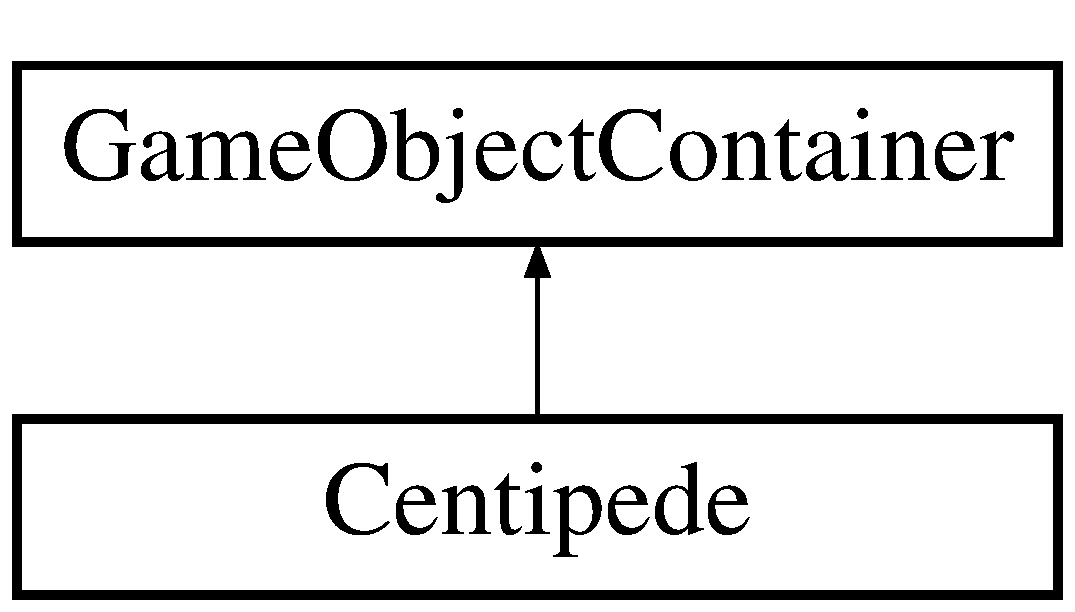
\includegraphics[height=2.000000cm]{class_centipede}
\end{center}
\end{figure}
\subsection*{Public Member Functions}
\begin{DoxyCompactItemize}
\item 
\mbox{\Hypertarget{class_centipede_a694d8add5c6962a8a89eb3e0a556d4a0}\label{class_centipede_a694d8add5c6962a8a89eb3e0a556d4a0}} 
\mbox{\hyperlink{class_centipede_a694d8add5c6962a8a89eb3e0a556d4a0}{Centipede}} (int length)
\begin{DoxyCompactList}\small\item\em Constructor accepts length of the \mbox{\hyperlink{class_centipede}{Centipede}} to be created. \end{DoxyCompactList}\item 
\mbox{\Hypertarget{class_centipede_ae460a56f2f7d875ffafa16166aa5d6b6}\label{class_centipede_ae460a56f2f7d875ffafa16166aa5d6b6}} 
void \mbox{\hyperlink{class_centipede_ae460a56f2f7d875ffafa16166aa5d6b6}{Move}} ()
\begin{DoxyCompactList}\small\item\em Moves \mbox{\hyperlink{class_centipede}{Centipede}} across screen. \end{DoxyCompactList}\item 
virtual shared\+\_\+ptr$<$ \mbox{\hyperlink{class_game_object}{Game\+Object}} $>$ \mbox{\hyperlink{class_centipede_ae722488780d0d19e63510647b5fe108c}{segment}} (int i) const override
\begin{DoxyCompactList}\small\item\em Returns the ith \mbox{\hyperlink{class_centi_segment}{Centi\+Segment}}. \end{DoxyCompactList}\item 
\mbox{\Hypertarget{class_centipede_a850f32fbd537efc5d226d48e04b91d7f}\label{class_centipede_a850f32fbd537efc5d226d48e04b91d7f}} 
void \mbox{\hyperlink{class_centipede_a850f32fbd537efc5d226d48e04b91d7f}{Segment\+Destroyed}} ()
\begin{DoxyCompactList}\small\item\em Count the number of destroyed Centi\+Segments. \end{DoxyCompactList}\item 
bool \mbox{\hyperlink{class_centipede_a3d69f0ef4b57cf4b9c1beb1284f2f738}{is\+Dead}} ()
\begin{DoxyCompactList}\small\item\em checks if \mbox{\hyperlink{class_centipede}{Centipede}} is dead \end{DoxyCompactList}\item 
\mbox{\Hypertarget{class_centipede_a1fa0123a0ea08fb9b76305ec67692793}\label{class_centipede_a1fa0123a0ea08fb9b76305ec67692793}} 
virtual void \mbox{\hyperlink{class_centipede_a1fa0123a0ea08fb9b76305ec67692793}{reset}} () override
\begin{DoxyCompactList}\small\item\em Reset centipede to initial conditions. \end{DoxyCompactList}\item 
\mbox{\Hypertarget{class_centipede_af887a67031a6c63897f3fad86a0076c2}\label{class_centipede_af887a67031a6c63897f3fad86a0076c2}} 
virtual \mbox{\hyperlink{class_centipede_af887a67031a6c63897f3fad86a0076c2}{$\sim$\+Centipede}} ()
\begin{DoxyCompactList}\small\item\em destroys the \mbox{\hyperlink{class_centipede}{Centipede}} Objects \end{DoxyCompactList}\end{DoxyCompactItemize}
\subsection*{Private Member Functions}
\begin{DoxyCompactItemize}
\item 
\mbox{\Hypertarget{class_centipede_a8e63cbd49eea28d05a47ff898a4cea66}\label{class_centipede_a8e63cbd49eea28d05a47ff898a4cea66}} 
void \mbox{\hyperlink{class_centipede_a8e63cbd49eea28d05a47ff898a4cea66}{initial\+Conditions}} ()
\begin{DoxyCompactList}\small\item\em reconstructs the \mbox{\hyperlink{class_centipede}{Centipede}} to initial Conditions \end{DoxyCompactList}\end{DoxyCompactItemize}
\subsection*{Private Attributes}
\begin{DoxyCompactItemize}
\item 
\mbox{\Hypertarget{class_centipede_ab1427df87d3fb7b723c0fb8dce7e1e1c}\label{class_centipede_ab1427df87d3fb7b723c0fb8dce7e1e1c}} 
vector$<$ shared\+\_\+ptr$<$ \mbox{\hyperlink{class_centi_segment}{Centi\+Segment}} $>$ $>$ {\bfseries centipede\+\_\+}
\item 
\mbox{\Hypertarget{class_centipede_a32527f4884c64cf17ea28310f9532f52}\label{class_centipede_a32527f4884c64cf17ea28310f9532f52}} 
int {\bfseries num\+Dead\+Segments\+\_\+}
\end{DoxyCompactItemize}


\subsection{Detailed Description}
\begin{DoxyDate}{Date}
08/10/2018 
\end{DoxyDate}


\subsection{Member Function Documentation}
\mbox{\Hypertarget{class_centipede_a3d69f0ef4b57cf4b9c1beb1284f2f738}\label{class_centipede_a3d69f0ef4b57cf4b9c1beb1284f2f738}} 
\index{Centipede@{Centipede}!is\+Dead@{is\+Dead}}
\index{is\+Dead@{is\+Dead}!Centipede@{Centipede}}
\subsubsection{\texorpdfstring{is\+Dead()}{isDead()}}
{\footnotesize\ttfamily bool Centipede\+::is\+Dead (\begin{DoxyParamCaption}{ }\end{DoxyParamCaption})\hspace{0.3cm}{\ttfamily [inline]}}



checks if \mbox{\hyperlink{class_centipede}{Centipede}} is dead 

\begin{DoxyReturn}{Returns}
boolean 
\end{DoxyReturn}
\mbox{\Hypertarget{class_centipede_ae722488780d0d19e63510647b5fe108c}\label{class_centipede_ae722488780d0d19e63510647b5fe108c}} 
\index{Centipede@{Centipede}!segment@{segment}}
\index{segment@{segment}!Centipede@{Centipede}}
\subsubsection{\texorpdfstring{segment()}{segment()}}
{\footnotesize\ttfamily virtual shared\+\_\+ptr$<$\mbox{\hyperlink{class_game_object}{Game\+Object}}$>$ Centipede\+::segment (\begin{DoxyParamCaption}\item[{int}]{i }\end{DoxyParamCaption}) const\hspace{0.3cm}{\ttfamily [inline]}, {\ttfamily [override]}, {\ttfamily [virtual]}}



Returns the ith \mbox{\hyperlink{class_centi_segment}{Centi\+Segment}}. 


\begin{DoxyParams}{Parameters}
{\em i} & is the ith \mbox{\hyperlink{class_centi_segment}{Centi\+Segment}} \\
\hline
\end{DoxyParams}
\begin{DoxyReturn}{Returns}
shared pointer to the ith \mbox{\hyperlink{class_centi_segment}{Centi\+Segment}} 
\end{DoxyReturn}


Implements \mbox{\hyperlink{class_game_object_container_affa50b43ca7b82d54055b6499e024aba}{Game\+Object\+Container}}.



The documentation for this class was generated from the following files\+:\begin{DoxyCompactItemize}
\item 
C\+:/\+Users/bvrad/\+Dropbox/\+Boikanyo/elen3009/\+P\+R\+O\+J\+E\+C\+T/2018-\/project-\/1386807-\/\+Radiokana-\/1427726-\/\+Sepuru/game-\/source-\/code/\mbox{\hyperlink{_centipede_8h}{Centipede.\+h}}\item 
C\+:/\+Users/bvrad/\+Dropbox/\+Boikanyo/elen3009/\+P\+R\+O\+J\+E\+C\+T/2018-\/project-\/1386807-\/\+Radiokana-\/1427726-\/\+Sepuru/game-\/source-\/code/Centipede.\+cpp\end{DoxyCompactItemize}

\hypertarget{class_centi_segment}{}\section{Centi\+Segment Class Reference}
\label{class_centi_segment}\index{Centi\+Segment@{Centi\+Segment}}


{\ttfamily \#include $<$Csegment.\+h$>$}

Inheritance diagram for Centi\+Segment\+:\begin{figure}[H]
\begin{center}
\leavevmode
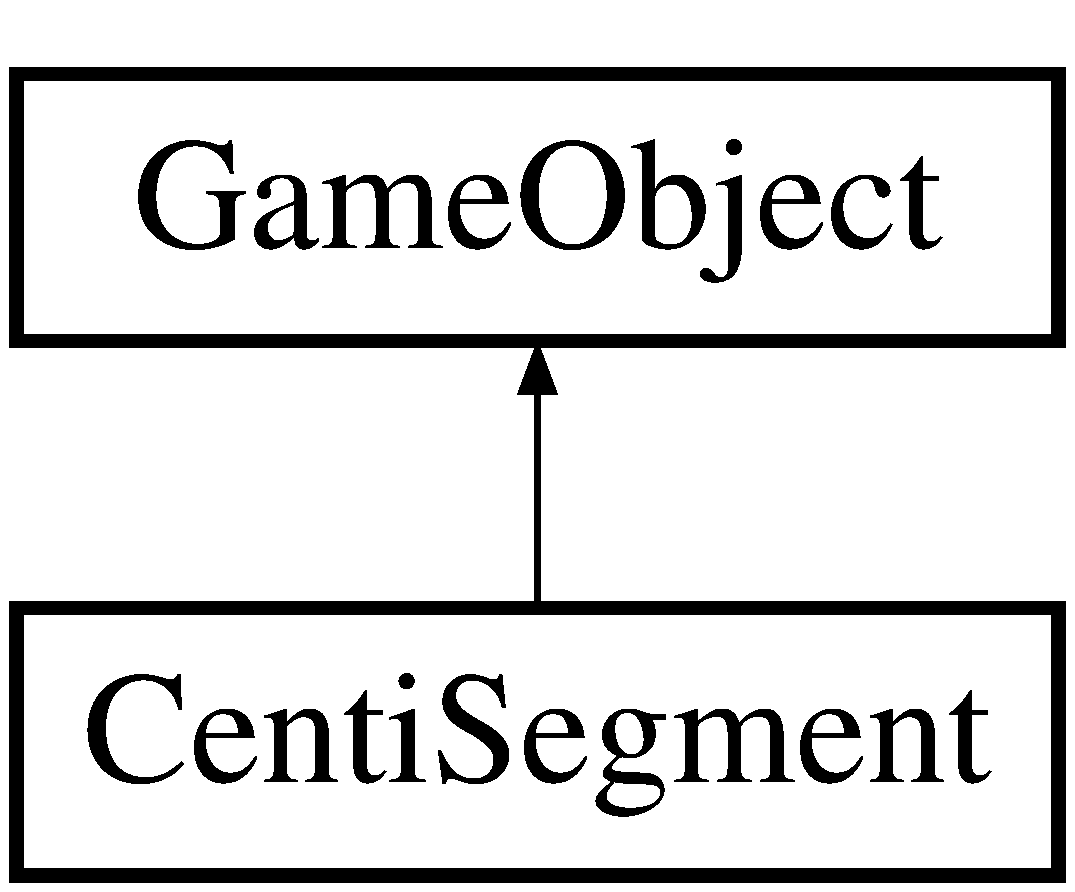
\includegraphics[height=2.000000cm]{class_centi_segment}
\end{center}
\end{figure}
\subsection*{Public Member Functions}
\begin{DoxyCompactItemize}
\item 
\mbox{\hyperlink{class_centi_segment_abfe286a4c657f151f8c149d88b94264c}{Centi\+Segment}} (const \mbox{\hyperlink{classvector2_d}{vector2D}} \&size, const \mbox{\hyperlink{classvector2_d}{vector2D}} \&position, float speed, Object\+ID objectid)
\begin{DoxyCompactList}\small\item\em Constructor of \mbox{\hyperlink{class_centi_segment}{Centi\+Segment}}. \end{DoxyCompactList}\item 
virtual void \mbox{\hyperlink{class_centi_segment_a7e1837a169b160e9a899504db13e4d2c}{Move}} () override
\item 
\mbox{\Hypertarget{class_centi_segment_ac657402352ec1276c76edd6d282d9a43}\label{class_centi_segment_ac657402352ec1276c76edd6d282d9a43}} 
virtual void \mbox{\hyperlink{class_centi_segment_ac657402352ec1276c76edd6d282d9a43}{reset}} () override
\begin{DoxyCompactList}\small\item\em set the centipede segment to its inital conditions \end{DoxyCompactList}\item 
virtual void \mbox{\hyperlink{class_centi_segment_a9161d48372e6c547ad5d5c630af0bfe4}{collision\+Response}} () override
\item 
\mbox{\Hypertarget{class_centi_segment_ae8b8e2a1e63374125b7f9913a8179e38}\label{class_centi_segment_ae8b8e2a1e63374125b7f9913a8179e38}} 
virtual \mbox{\hyperlink{class_centi_segment_ae8b8e2a1e63374125b7f9913a8179e38}{$\sim$\+Centi\+Segment}} ()
\begin{DoxyCompactList}\small\item\em Destroy the \mbox{\hyperlink{class_centi_segment}{Centi\+Segment}}. \end{DoxyCompactList}\end{DoxyCompactItemize}
\subsection*{Private Member Functions}
\begin{DoxyCompactItemize}
\item 
\mbox{\Hypertarget{class_centi_segment_ab6cdc9580f671fb06e62df3d78631125}\label{class_centi_segment_ab6cdc9580f671fb06e62df3d78631125}} 
void \mbox{\hyperlink{class_centi_segment_ab6cdc9580f671fb06e62df3d78631125}{move\+Left}} ()
\begin{DoxyCompactList}\small\item\em Move \mbox{\hyperlink{class_centi_segment}{Centi\+Segment}} Left. \end{DoxyCompactList}\item 
\mbox{\Hypertarget{class_centi_segment_aec29caa7fc59fa7db1661fb9dfc9c62a}\label{class_centi_segment_aec29caa7fc59fa7db1661fb9dfc9c62a}} 
void \mbox{\hyperlink{class_centi_segment_aec29caa7fc59fa7db1661fb9dfc9c62a}{move\+Right}} ()
\begin{DoxyCompactList}\small\item\em Move \mbox{\hyperlink{class_centi_segment}{Centi\+Segment}} Right. \end{DoxyCompactList}\item 
\mbox{\Hypertarget{class_centi_segment_a7238c16d6e8af24003f3d7321797c458}\label{class_centi_segment_a7238c16d6e8af24003f3d7321797c458}} 
void \mbox{\hyperlink{class_centi_segment_a7238c16d6e8af24003f3d7321797c458}{move\+Up}} ()
\begin{DoxyCompactList}\small\item\em Move \mbox{\hyperlink{class_centi_segment}{Centi\+Segment}} Up. \end{DoxyCompactList}\item 
\mbox{\Hypertarget{class_centi_segment_ac0d964dda7b0a21b08aeace080235dec}\label{class_centi_segment_ac0d964dda7b0a21b08aeace080235dec}} 
void \mbox{\hyperlink{class_centi_segment_ac0d964dda7b0a21b08aeace080235dec}{move\+Down}} ()
\begin{DoxyCompactList}\small\item\em Move \mbox{\hyperlink{class_centi_segment}{Centi\+Segment}} Down. \end{DoxyCompactList}\item 
\mbox{\Hypertarget{class_centi_segment_ad6437e55882b585549c94ef33fd1b80c}\label{class_centi_segment_ad6437e55882b585549c94ef33fd1b80c}} 
void \mbox{\hyperlink{class_centi_segment_ad6437e55882b585549c94ef33fd1b80c}{entrance}} ()
\begin{DoxyCompactList}\small\item\em entrance Movement \end{DoxyCompactList}\end{DoxyCompactItemize}
\subsection*{Private Attributes}
\begin{DoxyCompactItemize}
\item 
\mbox{\Hypertarget{class_centi_segment_ae586efde07494f87ea628d2e87fa1d87}\label{class_centi_segment_ae586efde07494f87ea628d2e87fa1d87}} 
bool {\bfseries forward\+\_\+} = true
\item 
\mbox{\Hypertarget{class_centi_segment_ae351cbdf46e19f61796cf106d0e8859e}\label{class_centi_segment_ae351cbdf46e19f61796cf106d0e8859e}} 
bool {\bfseries up\+\_\+} = false
\item 
\mbox{\Hypertarget{class_centi_segment_a22f79151305daec489c17bcb4fa7e553}\label{class_centi_segment_a22f79151305daec489c17bcb4fa7e553}} 
bool {\bfseries at\+Boundry\+\_\+} = false
\end{DoxyCompactItemize}


\subsection{Detailed Description}
\begin{DoxyDate}{Date}
08/10/2018 
\end{DoxyDate}


\subsection{Constructor \& Destructor Documentation}
\mbox{\Hypertarget{class_centi_segment_abfe286a4c657f151f8c149d88b94264c}\label{class_centi_segment_abfe286a4c657f151f8c149d88b94264c}} 
\index{Centi\+Segment@{Centi\+Segment}!Centi\+Segment@{Centi\+Segment}}
\index{Centi\+Segment@{Centi\+Segment}!Centi\+Segment@{Centi\+Segment}}
\subsubsection{\texorpdfstring{Centi\+Segment()}{CentiSegment()}}
{\footnotesize\ttfamily Centi\+Segment\+::\+Centi\+Segment (\begin{DoxyParamCaption}\item[{const \mbox{\hyperlink{classvector2_d}{vector2D}} \&}]{size,  }\item[{const \mbox{\hyperlink{classvector2_d}{vector2D}} \&}]{position,  }\item[{float}]{speed,  }\item[{Object\+ID}]{objectid }\end{DoxyParamCaption})\hspace{0.3cm}{\ttfamily [inline]}}



Constructor of \mbox{\hyperlink{class_centi_segment}{Centi\+Segment}}. 


\begin{DoxyParams}{Parameters}
{\em size} & of the \mbox{\hyperlink{class_centi_segment}{Centi\+Segment}} \\
\hline
{\em position} & of the \mbox{\hyperlink{class_centi_segment}{Centi\+Segment}} \\
\hline
{\em speed} & of the \mbox{\hyperlink{class_centi_segment}{Centi\+Segment}} \\
\hline
{\em objectid} & ID of the \mbox{\hyperlink{class_centi_segment}{Centi\+Segment}} \\
\hline
\end{DoxyParams}


\subsection{Member Function Documentation}
\mbox{\Hypertarget{class_centi_segment_a9161d48372e6c547ad5d5c630af0bfe4}\label{class_centi_segment_a9161d48372e6c547ad5d5c630af0bfe4}} 
\index{Centi\+Segment@{Centi\+Segment}!collision\+Response@{collision\+Response}}
\index{collision\+Response@{collision\+Response}!Centi\+Segment@{Centi\+Segment}}
\subsubsection{\texorpdfstring{collision\+Response()}{collisionResponse()}}
{\footnotesize\ttfamily void Centi\+Segment\+::collision\+Response (\begin{DoxyParamCaption}{ }\end{DoxyParamCaption})\hspace{0.3cm}{\ttfamily [override]}, {\ttfamily [virtual]}}

Take action if hits a mushroom 

Implements \mbox{\hyperlink{class_game_object_aafcceed70da5ea5971b82843ea9222e9}{Game\+Object}}.

\mbox{\Hypertarget{class_centi_segment_a7e1837a169b160e9a899504db13e4d2c}\label{class_centi_segment_a7e1837a169b160e9a899504db13e4d2c}} 
\index{Centi\+Segment@{Centi\+Segment}!Move@{Move}}
\index{Move@{Move}!Centi\+Segment@{Centi\+Segment}}
\subsubsection{\texorpdfstring{Move()}{Move()}}
{\footnotesize\ttfamily void Centi\+Segment\+::\+Move (\begin{DoxyParamCaption}{ }\end{DoxyParamCaption})\hspace{0.3cm}{\ttfamily [override]}, {\ttfamily [virtual]}}

the \mbox{\hyperlink{class_centi_segment}{Centi\+Segment}} across the screen 

Implements \mbox{\hyperlink{class_game_object_a4bc279e0b3da8273e4e869cc7584847d}{Game\+Object}}.



The documentation for this class was generated from the following files\+:\begin{DoxyCompactItemize}
\item 
C\+:/\+Users/bvrad/\+Dropbox/\+Boikanyo/elen3009/\+P\+R\+O\+J\+E\+C\+T/2018-\/project-\/1386807-\/\+Radiokana-\/1427726-\/\+Sepuru/game-\/source-\/code/\mbox{\hyperlink{_csegment_8h}{Csegment.\+h}}\item 
C\+:/\+Users/bvrad/\+Dropbox/\+Boikanyo/elen3009/\+P\+R\+O\+J\+E\+C\+T/2018-\/project-\/1386807-\/\+Radiokana-\/1427726-\/\+Sepuru/game-\/source-\/code/Csegment.\+cpp\end{DoxyCompactItemize}

\hypertarget{class_collision}{}\section{Collision Class Reference}
\label{class_collision}\index{Collision@{Collision}}


{\ttfamily \#include $<$Collision.\+h$>$}

\subsection*{Public Member Functions}
\begin{DoxyCompactItemize}
\item 
bool \mbox{\hyperlink{class_collision_a43e40b319ff4d328b467877ab39710d5}{check\+Collision}} (shared\+\_\+ptr$<$ \mbox{\hyperlink{class_game_object}{Game\+Object}} $>$ this\+\_\+ptr, shared\+\_\+ptr$<$ \mbox{\hyperlink{class_game_object}{Game\+Object}} $>$ other\+\_\+ptr)
\begin{DoxyCompactList}\small\item\em checks if two Game\+Objects overlap \end{DoxyCompactList}\item 
\mbox{\Hypertarget{class_collision_a19ae49bcb3b16f4622443a34a171590c}\label{class_collision_a19ae49bcb3b16f4622443a34a171590c}} 
\mbox{\hyperlink{class_collision_a19ae49bcb3b16f4622443a34a171590c}{$\sim$\+Collision}} ()
\begin{DoxyCompactList}\small\item\em Destroys the Collison object. \end{DoxyCompactList}\end{DoxyCompactItemize}


\subsection{Detailed Description}
\begin{DoxyDate}{Date}
08/10/2018 
\end{DoxyDate}


\subsection{Member Function Documentation}
\mbox{\Hypertarget{class_collision_a43e40b319ff4d328b467877ab39710d5}\label{class_collision_a43e40b319ff4d328b467877ab39710d5}} 
\index{Collision@{Collision}!check\+Collision@{check\+Collision}}
\index{check\+Collision@{check\+Collision}!Collision@{Collision}}
\subsubsection{\texorpdfstring{check\+Collision()}{checkCollision()}}
{\footnotesize\ttfamily bool Collision\+::check\+Collision (\begin{DoxyParamCaption}\item[{shared\+\_\+ptr$<$ \mbox{\hyperlink{class_game_object}{Game\+Object}} $>$}]{this\+\_\+ptr,  }\item[{shared\+\_\+ptr$<$ \mbox{\hyperlink{class_game_object}{Game\+Object}} $>$}]{other\+\_\+ptr }\end{DoxyParamCaption})}



checks if two Game\+Objects overlap 


\begin{DoxyParams}{Parameters}
{\em this\+\_\+ptr} & the \mbox{\hyperlink{class_game_object}{Game\+Object}} colliding \\
\hline
{\em other\+\_\+ptr} & the Game\+Objects is colliding with \\
\hline
\end{DoxyParams}
\begin{DoxyReturn}{Returns}
boolean signaling collision or not 
\end{DoxyReturn}


The documentation for this class was generated from the following files\+:\begin{DoxyCompactItemize}
\item 
C\+:/\+Users/bvrad/\+Dropbox/\+Boikanyo/elen3009/\+P\+R\+O\+J\+E\+C\+T/2018-\/project-\/1386807-\/\+Radiokana-\/1427726-\/\+Sepuru/game-\/source-\/code/\mbox{\hyperlink{_collision_8h}{Collision.\+h}}\item 
C\+:/\+Users/bvrad/\+Dropbox/\+Boikanyo/elen3009/\+P\+R\+O\+J\+E\+C\+T/2018-\/project-\/1386807-\/\+Radiokana-\/1427726-\/\+Sepuru/game-\/source-\/code/Collision.\+cpp\end{DoxyCompactItemize}

\hypertarget{class_collision_handler}{}\section{Collision\+Handler Class Reference}
\label{class_collision_handler}\index{Collision\+Handler@{Collision\+Handler}}


{\ttfamily \#include $<$Collision\+Handler.\+h$>$}

\subsection*{Public Member Functions}
\begin{DoxyCompactItemize}
\item 
\mbox{\hyperlink{class_collision_handler_ad7e987b02f093a6c060b3b9396a323ce}{Collision\+Handler}} (shared\+\_\+ptr$<$ \mbox{\hyperlink{class_score}{Score}} $>$ score\+\_\+ptr)
\begin{DoxyCompactList}\small\item\em Constructor initializes the collision objects, the two classes share a composition relationship. \end{DoxyCompactList}\item 
void \mbox{\hyperlink{class_collision_handler_a38653a91128ac260d2571be8d40c48bf}{target\+Destroyed}} (shared\+\_\+ptr$<$ \mbox{\hyperlink{class_spaceship}{Spaceship}} $>$ spaceship\+\_\+ptr, shared\+\_\+ptr$<$ \mbox{\hyperlink{class_centipede}{Centipede}} $>$ centipede\+\_\+ptr, shared\+\_\+ptr$<$ \mbox{\hyperlink{class_mushroom_field}{Mushroom\+Field}} $>$ mushroom\+\_\+ptr)
\begin{DoxyCompactList}\small\item\em Handle \mbox{\hyperlink{class_lazer_shot}{Lazer\+Shot}} and \mbox{\hyperlink{class_centipede}{Centipede}} Collisons. \end{DoxyCompactList}\item 
void \mbox{\hyperlink{class_collision_handler_a7bdf9fae4c9da0cbb46e43db1326c73a}{spaceship\+Hit}} (shared\+\_\+ptr$<$ \mbox{\hyperlink{class_centipede}{Centipede}} $>$ centipede\+\_\+ptr, shared\+\_\+ptr$<$ \mbox{\hyperlink{class_spaceship}{Spaceship}} $>$ spaceship\+\_\+ptr)
\begin{DoxyCompactList}\small\item\em Handle \mbox{\hyperlink{class_centipede}{Centipede}} and \mbox{\hyperlink{class_spaceship}{Spaceship}} Collison. \end{DoxyCompactList}\item 
void \mbox{\hyperlink{class_collision_handler_ae442cd4e1b0383607873a09c2be2bf13}{mushroom\+Hit}} (shared\+\_\+ptr$<$ \mbox{\hyperlink{class_centipede}{Centipede}} $>$ centipede\+\_\+ptr, shared\+\_\+ptr$<$ \mbox{\hyperlink{class_mushroom_field}{Mushroom\+Field}} $>$ mushroom\+\_\+ptr)
\begin{DoxyCompactList}\small\item\em Handle \mbox{\hyperlink{class_centipede}{Centipede}} and \mbox{\hyperlink{class_mushroom}{Mushroom}} collission. \end{DoxyCompactList}\item 
void \mbox{\hyperlink{class_collision_handler_af63977ae014e8013b2beca67ab3d22cf}{mushroom\+Shot}} (shared\+\_\+ptr$<$ \mbox{\hyperlink{class_spaceship}{Spaceship}} $>$ spaceship\+\_\+ptr, shared\+\_\+ptr$<$ \mbox{\hyperlink{class_mushroom_field}{Mushroom\+Field}} $>$ mushroom\+\_\+ptr)
\begin{DoxyCompactList}\small\item\em Handle \mbox{\hyperlink{class_mushroom}{Mushroom}} Bullet \mbox{\hyperlink{class_collision}{Collision}}. \end{DoxyCompactList}\item 
void \mbox{\hyperlink{class_collision_handler_a709eb0dd73f96ce7aff7fbd7deaa8355}{spaceship\+Collision}} (shared\+\_\+ptr$<$ \mbox{\hyperlink{class_spaceship}{Spaceship}} $>$ spaceship\+\_\+ptr, shared\+\_\+ptr$<$ \mbox{\hyperlink{class_mushroom_field}{Mushroom\+Field}} $>$ mushroom\+\_\+ptr, shared\+\_\+ptr$<$ \mbox{\hyperlink{class_player}{Player}} $>$ player\+\_\+ptr)
\begin{DoxyCompactList}\small\item\em Handle \mbox{\hyperlink{class_spaceship}{Spaceship}} mushroom collision. \end{DoxyCompactList}\item 
void \mbox{\hyperlink{class_collision_handler_abb75bc290df29ec796f0869329b61a1e}{spaceship\+Hit}} (shared\+\_\+ptr$<$ \mbox{\hyperlink{class_spider}{Spider}} $>$ spider\+\_\+ptr, shared\+\_\+ptr$<$ \mbox{\hyperlink{class_spaceship}{Spaceship}} $>$ spaceship\+\_\+ptr)
\begin{DoxyCompactList}\small\item\em Handle \mbox{\hyperlink{class_collision}{Collision}} between \mbox{\hyperlink{class_spider}{Spider}} and \mbox{\hyperlink{class_spaceship}{Spaceship}}. \end{DoxyCompactList}\item 
void \mbox{\hyperlink{class_collision_handler_a314663c4aa7a14e7b935794796e6e7c5}{mushroom\+Destroyed}} (shared\+\_\+ptr$<$ \mbox{\hyperlink{class_game_object}{Game\+Object}} $>$ game\+Object\+\_\+ptr, shared\+\_\+ptr$<$ \mbox{\hyperlink{class_game_object_container}{Game\+Object\+Container}} $>$ game\+Object\+Container\+\_\+ptr)
\begin{DoxyCompactList}\small\item\em Handle \mbox{\hyperlink{class_spider}{Spider}} \mbox{\hyperlink{class_mushroom}{Mushroom}} \mbox{\hyperlink{class_collision}{Collision}}. \end{DoxyCompactList}\item 
void \mbox{\hyperlink{class_collision_handler_aba8e483266434721d8914aa10ae20797}{target\+Destroyed}} (shared\+\_\+ptr$<$ \mbox{\hyperlink{class_spaceship}{Spaceship}} $>$ spaceship\+\_\+ptr, shared\+\_\+ptr$<$ \mbox{\hyperlink{class_spider}{Spider}} $>$ spider\+\_\+ptr)
\begin{DoxyCompactList}\small\item\em Handle spider Lazershot Collison. \end{DoxyCompactList}\item 
void \mbox{\hyperlink{class_collision_handler_a8691ccab3aa2d3b300b8982b5c38acc3}{target\+Destroyed}} (shared\+\_\+ptr$<$ \mbox{\hyperlink{class_spaceship}{Spaceship}} $>$ spaceship\+\_\+ptr, shared\+\_\+ptr$<$ \mbox{\hyperlink{class_scorpion}{Scorpion}} $>$ scorpion\+\_\+ptr)
\begin{DoxyCompactList}\small\item\em Handle \mbox{\hyperlink{class_scorpion}{Scorpion}} \mbox{\hyperlink{class_lazer_shot}{Lazer\+Shot}} Colliosn. \end{DoxyCompactList}\item 
\mbox{\Hypertarget{class_collision_handler_a99f5524cf1706f9ea95500cf273a9d97}\label{class_collision_handler_a99f5524cf1706f9ea95500cf273a9d97}} 
\mbox{\hyperlink{class_collision_handler_a99f5524cf1706f9ea95500cf273a9d97}{$\sim$\+Collision\+Handler}} ()
\begin{DoxyCompactList}\small\item\em Destroy \mbox{\hyperlink{class_collision_handler}{Collision\+Handler}} Object. \end{DoxyCompactList}\end{DoxyCompactItemize}
\subsection*{Private Attributes}
\begin{DoxyCompactItemize}
\item 
\mbox{\Hypertarget{class_collision_handler_abe0be81527d73f773f9d388f44efc536}\label{class_collision_handler_abe0be81527d73f773f9d388f44efc536}} 
shared\+\_\+ptr$<$ \mbox{\hyperlink{class_score}{Score}} $>$ {\bfseries \+\_\+score\+\_\+ptr}
\item 
\mbox{\Hypertarget{class_collision_handler_af0c7e6de35e6c07fd9a1115c11adb478}\label{class_collision_handler_af0c7e6de35e6c07fd9a1115c11adb478}} 
unique\+\_\+ptr$<$ \mbox{\hyperlink{class_collision}{Collision}} $>$ {\bfseries \+\_\+collision\+\_\+ptr}
\end{DoxyCompactItemize}


\subsection{Detailed Description}
\begin{DoxyDate}{Date}
08/10/2018 
\end{DoxyDate}


\subsection{Constructor \& Destructor Documentation}
\mbox{\Hypertarget{class_collision_handler_ad7e987b02f093a6c060b3b9396a323ce}\label{class_collision_handler_ad7e987b02f093a6c060b3b9396a323ce}} 
\index{Collision\+Handler@{Collision\+Handler}!Collision\+Handler@{Collision\+Handler}}
\index{Collision\+Handler@{Collision\+Handler}!Collision\+Handler@{Collision\+Handler}}
\subsubsection{\texorpdfstring{Collision\+Handler()}{CollisionHandler()}}
{\footnotesize\ttfamily Collision\+Handler\+::\+Collision\+Handler (\begin{DoxyParamCaption}\item[{shared\+\_\+ptr$<$ \mbox{\hyperlink{class_score}{Score}} $>$}]{score\+\_\+ptr }\end{DoxyParamCaption})\hspace{0.3cm}{\ttfamily [inline]}}



Constructor initializes the collision objects, the two classes share a composition relationship. 


\begin{DoxyParams}{Parameters}
{\em score\+\_\+ptr} & to calculate score \\
\hline
\end{DoxyParams}


\subsection{Member Function Documentation}
\mbox{\Hypertarget{class_collision_handler_a314663c4aa7a14e7b935794796e6e7c5}\label{class_collision_handler_a314663c4aa7a14e7b935794796e6e7c5}} 
\index{Collision\+Handler@{Collision\+Handler}!mushroom\+Destroyed@{mushroom\+Destroyed}}
\index{mushroom\+Destroyed@{mushroom\+Destroyed}!Collision\+Handler@{Collision\+Handler}}
\subsubsection{\texorpdfstring{mushroom\+Destroyed()}{mushroomDestroyed()}}
{\footnotesize\ttfamily void Collision\+Handler\+::mushroom\+Destroyed (\begin{DoxyParamCaption}\item[{shared\+\_\+ptr$<$ \mbox{\hyperlink{class_game_object}{Game\+Object}} $>$}]{game\+Object\+\_\+ptr,  }\item[{shared\+\_\+ptr$<$ \mbox{\hyperlink{class_game_object_container}{Game\+Object\+Container}} $>$}]{game\+Object\+Container\+\_\+ptr }\end{DoxyParamCaption})}



Handle \mbox{\hyperlink{class_spider}{Spider}} \mbox{\hyperlink{class_mushroom}{Mushroom}} \mbox{\hyperlink{class_collision}{Collision}}. 


\begin{DoxyParams}{Parameters}
{\em game\+Object\+\_\+ptr} & pointer to \mbox{\hyperlink{class_game_object}{Game\+Object}} \\
\hline
{\em game\+Object\+Container\+\_\+ptr} & pointer to \mbox{\hyperlink{class_game_object_container}{Game\+Object\+Container}} \\
\hline
\end{DoxyParams}
\mbox{\Hypertarget{class_collision_handler_ae442cd4e1b0383607873a09c2be2bf13}\label{class_collision_handler_ae442cd4e1b0383607873a09c2be2bf13}} 
\index{Collision\+Handler@{Collision\+Handler}!mushroom\+Hit@{mushroom\+Hit}}
\index{mushroom\+Hit@{mushroom\+Hit}!Collision\+Handler@{Collision\+Handler}}
\subsubsection{\texorpdfstring{mushroom\+Hit()}{mushroomHit()}}
{\footnotesize\ttfamily void Collision\+Handler\+::mushroom\+Hit (\begin{DoxyParamCaption}\item[{shared\+\_\+ptr$<$ \mbox{\hyperlink{class_centipede}{Centipede}} $>$}]{centipede\+\_\+ptr,  }\item[{shared\+\_\+ptr$<$ \mbox{\hyperlink{class_mushroom_field}{Mushroom\+Field}} $>$}]{mushroom\+\_\+ptr }\end{DoxyParamCaption})}



Handle \mbox{\hyperlink{class_centipede}{Centipede}} and \mbox{\hyperlink{class_mushroom}{Mushroom}} collission. 


\begin{DoxyParams}{Parameters}
{\em centipede\+\_\+ptr} & pointer to the \mbox{\hyperlink{class_centipede}{Centipede}} object \\
\hline
{\em mushroom\+\_\+ptr} & pointer to the \mbox{\hyperlink{class_mushroom_field}{Mushroom\+Field}} object \\
\hline
\end{DoxyParams}
\mbox{\Hypertarget{class_collision_handler_af63977ae014e8013b2beca67ab3d22cf}\label{class_collision_handler_af63977ae014e8013b2beca67ab3d22cf}} 
\index{Collision\+Handler@{Collision\+Handler}!mushroom\+Shot@{mushroom\+Shot}}
\index{mushroom\+Shot@{mushroom\+Shot}!Collision\+Handler@{Collision\+Handler}}
\subsubsection{\texorpdfstring{mushroom\+Shot()}{mushroomShot()}}
{\footnotesize\ttfamily void Collision\+Handler\+::mushroom\+Shot (\begin{DoxyParamCaption}\item[{shared\+\_\+ptr$<$ \mbox{\hyperlink{class_spaceship}{Spaceship}} $>$}]{spaceship\+\_\+ptr,  }\item[{shared\+\_\+ptr$<$ \mbox{\hyperlink{class_mushroom_field}{Mushroom\+Field}} $>$}]{mushroom\+\_\+ptr }\end{DoxyParamCaption})}



Handle \mbox{\hyperlink{class_mushroom}{Mushroom}} Bullet \mbox{\hyperlink{class_collision}{Collision}}. 


\begin{DoxyParams}{Parameters}
{\em spaceship\+\_\+ptr} & pointer to the \mbox{\hyperlink{class_spaceship}{Spaceship}} object \\
\hline
{\em mushroom\+\_\+ptr} & pointer to the \mbox{\hyperlink{class_mushroom_field}{Mushroom\+Field}} object \\
\hline
\end{DoxyParams}
\mbox{\Hypertarget{class_collision_handler_a709eb0dd73f96ce7aff7fbd7deaa8355}\label{class_collision_handler_a709eb0dd73f96ce7aff7fbd7deaa8355}} 
\index{Collision\+Handler@{Collision\+Handler}!spaceship\+Collision@{spaceship\+Collision}}
\index{spaceship\+Collision@{spaceship\+Collision}!Collision\+Handler@{Collision\+Handler}}
\subsubsection{\texorpdfstring{spaceship\+Collision()}{spaceshipCollision()}}
{\footnotesize\ttfamily void Collision\+Handler\+::spaceship\+Collision (\begin{DoxyParamCaption}\item[{shared\+\_\+ptr$<$ \mbox{\hyperlink{class_spaceship}{Spaceship}} $>$}]{spaceship\+\_\+ptr,  }\item[{shared\+\_\+ptr$<$ \mbox{\hyperlink{class_mushroom_field}{Mushroom\+Field}} $>$}]{mushroom\+\_\+ptr,  }\item[{shared\+\_\+ptr$<$ \mbox{\hyperlink{class_player}{Player}} $>$}]{player\+\_\+ptr }\end{DoxyParamCaption})}



Handle \mbox{\hyperlink{class_spaceship}{Spaceship}} mushroom collision. 


\begin{DoxyParams}{Parameters}
{\em spaceship\+\_\+ptr} & pointer to the \mbox{\hyperlink{class_spaceship}{Spaceship}} object \\
\hline
{\em mushroom\+\_\+ptr} & pointer to the \mbox{\hyperlink{class_mushroom_field}{Mushroom\+Field}} object \\
\hline
{\em player\+\_\+ptr} & pointer to the player object \\
\hline
\end{DoxyParams}
\mbox{\Hypertarget{class_collision_handler_a7bdf9fae4c9da0cbb46e43db1326c73a}\label{class_collision_handler_a7bdf9fae4c9da0cbb46e43db1326c73a}} 
\index{Collision\+Handler@{Collision\+Handler}!spaceship\+Hit@{spaceship\+Hit}}
\index{spaceship\+Hit@{spaceship\+Hit}!Collision\+Handler@{Collision\+Handler}}
\subsubsection{\texorpdfstring{spaceship\+Hit()}{spaceshipHit()}\hspace{0.1cm}{\footnotesize\ttfamily [1/2]}}
{\footnotesize\ttfamily void Collision\+Handler\+::spaceship\+Hit (\begin{DoxyParamCaption}\item[{shared\+\_\+ptr$<$ \mbox{\hyperlink{class_centipede}{Centipede}} $>$}]{centipede\+\_\+ptr,  }\item[{shared\+\_\+ptr$<$ \mbox{\hyperlink{class_spaceship}{Spaceship}} $>$}]{spaceship\+\_\+ptr }\end{DoxyParamCaption})}



Handle \mbox{\hyperlink{class_centipede}{Centipede}} and \mbox{\hyperlink{class_spaceship}{Spaceship}} Collison. 


\begin{DoxyParams}{Parameters}
{\em centipede\+\_\+ptr} & pointer to the \mbox{\hyperlink{class_centipede}{Centipede}} object \\
\hline
{\em spaceship\+\_\+ptr} & pointer to the \mbox{\hyperlink{class_spaceship}{Spaceship}} object \\
\hline
\end{DoxyParams}
\mbox{\Hypertarget{class_collision_handler_abb75bc290df29ec796f0869329b61a1e}\label{class_collision_handler_abb75bc290df29ec796f0869329b61a1e}} 
\index{Collision\+Handler@{Collision\+Handler}!spaceship\+Hit@{spaceship\+Hit}}
\index{spaceship\+Hit@{spaceship\+Hit}!Collision\+Handler@{Collision\+Handler}}
\subsubsection{\texorpdfstring{spaceship\+Hit()}{spaceshipHit()}\hspace{0.1cm}{\footnotesize\ttfamily [2/2]}}
{\footnotesize\ttfamily void Collision\+Handler\+::spaceship\+Hit (\begin{DoxyParamCaption}\item[{shared\+\_\+ptr$<$ \mbox{\hyperlink{class_spider}{Spider}} $>$}]{spider\+\_\+ptr,  }\item[{shared\+\_\+ptr$<$ \mbox{\hyperlink{class_spaceship}{Spaceship}} $>$}]{spaceship\+\_\+ptr }\end{DoxyParamCaption})}



Handle \mbox{\hyperlink{class_collision}{Collision}} between \mbox{\hyperlink{class_spider}{Spider}} and \mbox{\hyperlink{class_spaceship}{Spaceship}}. 


\begin{DoxyParams}{Parameters}
{\em spider\+\_\+ptr} & pointer to the spider object \\
\hline
{\em spaceship\+\_\+ptr} & pointer to the \mbox{\hyperlink{class_spaceship}{Spaceship}} object \\
\hline
\end{DoxyParams}
\mbox{\Hypertarget{class_collision_handler_a38653a91128ac260d2571be8d40c48bf}\label{class_collision_handler_a38653a91128ac260d2571be8d40c48bf}} 
\index{Collision\+Handler@{Collision\+Handler}!target\+Destroyed@{target\+Destroyed}}
\index{target\+Destroyed@{target\+Destroyed}!Collision\+Handler@{Collision\+Handler}}
\subsubsection{\texorpdfstring{target\+Destroyed()}{targetDestroyed()}\hspace{0.1cm}{\footnotesize\ttfamily [1/3]}}
{\footnotesize\ttfamily void Collision\+Handler\+::target\+Destroyed (\begin{DoxyParamCaption}\item[{shared\+\_\+ptr$<$ \mbox{\hyperlink{class_spaceship}{Spaceship}} $>$}]{spaceship\+\_\+ptr,  }\item[{shared\+\_\+ptr$<$ \mbox{\hyperlink{class_centipede}{Centipede}} $>$}]{centipede\+\_\+ptr,  }\item[{shared\+\_\+ptr$<$ \mbox{\hyperlink{class_mushroom_field}{Mushroom\+Field}} $>$}]{mushroom\+\_\+ptr }\end{DoxyParamCaption})}



Handle \mbox{\hyperlink{class_lazer_shot}{Lazer\+Shot}} and \mbox{\hyperlink{class_centipede}{Centipede}} Collisons. 


\begin{DoxyParams}{Parameters}
{\em spaceship\+\_\+ptr} & pointer to the \mbox{\hyperlink{class_spaceship}{Spaceship}} object \\
\hline
{\em centipede\+\_\+ptr} & pointer to the \mbox{\hyperlink{class_centipede}{Centipede}} object \\
\hline
{\em mushroom\+\_\+ptr} & pointer to the \mbox{\hyperlink{class_mushroom_field}{Mushroom\+Field}} object \\
\hline
\end{DoxyParams}
\mbox{\Hypertarget{class_collision_handler_aba8e483266434721d8914aa10ae20797}\label{class_collision_handler_aba8e483266434721d8914aa10ae20797}} 
\index{Collision\+Handler@{Collision\+Handler}!target\+Destroyed@{target\+Destroyed}}
\index{target\+Destroyed@{target\+Destroyed}!Collision\+Handler@{Collision\+Handler}}
\subsubsection{\texorpdfstring{target\+Destroyed()}{targetDestroyed()}\hspace{0.1cm}{\footnotesize\ttfamily [2/3]}}
{\footnotesize\ttfamily void Collision\+Handler\+::target\+Destroyed (\begin{DoxyParamCaption}\item[{shared\+\_\+ptr$<$ \mbox{\hyperlink{class_spaceship}{Spaceship}} $>$}]{spaceship\+\_\+ptr,  }\item[{shared\+\_\+ptr$<$ \mbox{\hyperlink{class_spider}{Spider}} $>$}]{spider\+\_\+ptr }\end{DoxyParamCaption})}



Handle spider Lazershot Collison. 


\begin{DoxyParams}{Parameters}
{\em spaceship\+\_\+ptr} & pointer to the \mbox{\hyperlink{class_spaceship}{Spaceship}} object shooting Lazer\+Shots \\
\hline
{\em spider\+\_\+ptr} & pointer to the spider object \\
\hline
\end{DoxyParams}
\mbox{\Hypertarget{class_collision_handler_a8691ccab3aa2d3b300b8982b5c38acc3}\label{class_collision_handler_a8691ccab3aa2d3b300b8982b5c38acc3}} 
\index{Collision\+Handler@{Collision\+Handler}!target\+Destroyed@{target\+Destroyed}}
\index{target\+Destroyed@{target\+Destroyed}!Collision\+Handler@{Collision\+Handler}}
\subsubsection{\texorpdfstring{target\+Destroyed()}{targetDestroyed()}\hspace{0.1cm}{\footnotesize\ttfamily [3/3]}}
{\footnotesize\ttfamily void Collision\+Handler\+::target\+Destroyed (\begin{DoxyParamCaption}\item[{shared\+\_\+ptr$<$ \mbox{\hyperlink{class_spaceship}{Spaceship}} $>$}]{spaceship\+\_\+ptr,  }\item[{shared\+\_\+ptr$<$ \mbox{\hyperlink{class_scorpion}{Scorpion}} $>$}]{scorpion\+\_\+ptr }\end{DoxyParamCaption})}



Handle \mbox{\hyperlink{class_scorpion}{Scorpion}} \mbox{\hyperlink{class_lazer_shot}{Lazer\+Shot}} Colliosn. 


\begin{DoxyParams}{Parameters}
{\em spaceship\+\_\+ptr} & pointer to the \mbox{\hyperlink{class_spaceship}{Spaceship}} object shooting Lazer\+Shots \\
\hline
{\em scorpion\+\_\+ptr} & pointer to \mbox{\hyperlink{class_scorpion}{Scorpion}} object \\
\hline
\end{DoxyParams}


The documentation for this class was generated from the following files\+:\begin{DoxyCompactItemize}
\item 
C\+:/\+Users/bvrad/\+Dropbox/\+Boikanyo/elen3009/\+P\+R\+O\+J\+E\+C\+T/2018-\/project-\/1386807-\/\+Radiokana-\/1427726-\/\+Sepuru/game-\/source-\/code/\mbox{\hyperlink{_collision_handler_8h}{Collision\+Handler.\+h}}\item 
C\+:/\+Users/bvrad/\+Dropbox/\+Boikanyo/elen3009/\+P\+R\+O\+J\+E\+C\+T/2018-\/project-\/1386807-\/\+Radiokana-\/1427726-\/\+Sepuru/game-\/source-\/code/Collision\+Handler.\+cpp\end{DoxyCompactItemize}

\hypertarget{class_display}{}\section{Display Class Reference}
\label{class_display}\index{Display@{Display}}


{\ttfamily \#include $<$Display.\+h$>$}

\subsection*{Public Member Functions}
\begin{DoxyCompactItemize}
\item 
\mbox{\Hypertarget{class_display_aeb2f7390982338b48d8bb9a61f159bc3}\label{class_display_aeb2f7390982338b48d8bb9a61f159bc3}} 
\mbox{\hyperlink{class_display_aeb2f7390982338b48d8bb9a61f159bc3}{Display}} (float screen\+Width, float Screen\+Height)
\begin{DoxyCompactList}\small\item\em initialize the \mbox{\hyperlink{class_display}{Display}} \end{DoxyCompactList}\item 
\mbox{\Hypertarget{class_display_aa3ab70ec7b76fa3ed139d19e53e72283}\label{class_display_aa3ab70ec7b76fa3ed139d19e53e72283}} 
void \mbox{\hyperlink{class_display_aa3ab70ec7b76fa3ed139d19e53e72283}{display}} ()
\begin{DoxyCompactList}\small\item\em \mbox{\hyperlink{class_display}{Display}} drawn object on display. \end{DoxyCompactList}\item 
bool \mbox{\hyperlink{class_display_a2d8a021131e48ba0388c24754dd5286c}{space\+Key}} ()
\begin{DoxyCompactList}\small\item\em Check for the press of space key. \end{DoxyCompactList}\item 
void \mbox{\hyperlink{class_display_afd34049cad61f21d56f8d64c53282cea}{Events}} (shared\+\_\+ptr$<$ \mbox{\hyperlink{class_user_inputs}{User\+Inputs}} $>$ userinput\+\_\+ptr)
\begin{DoxyCompactList}\small\item\em Poll for events. \end{DoxyCompactList}\item 
bool \mbox{\hyperlink{class_display_a45a76d7780b8b35251a4510849cd58e8}{is\+Open}} () const
\begin{DoxyCompactList}\small\item\em Check if \mbox{\hyperlink{class_display}{Display}} is Open. \end{DoxyCompactList}\item 
bool \mbox{\hyperlink{class_display_a1b81707d811188dbfd98be312679223f}{left\+Click}} ()
\begin{DoxyCompactList}\small\item\em Check if mouse is clicked on the left side. \end{DoxyCompactList}\item 
\mbox{\Hypertarget{class_display_a9ce27466645f406154c1e48f4cbe5857}\label{class_display_a9ce27466645f406154c1e48f4cbe5857}} 
void \mbox{\hyperlink{class_display_a9ce27466645f406154c1e48f4cbe5857}{clear\+Display}} ()
\begin{DoxyCompactList}\small\item\em Clear the window. \end{DoxyCompactList}\item 
shared\+\_\+ptr$<$ sf\+::\+Render\+Window $>$ \mbox{\hyperlink{class_display_a5e7a8c62af3817bbd66c7727943bbef9}{window}} ()
\begin{DoxyCompactList}\small\item\em return a shared pointer to the window \end{DoxyCompactList}\item 
void \mbox{\hyperlink{class_display_ab1de6d8b7911336e30999b78f3f6cbe3}{delayer}} (tuple$<$ bool, bool, bool $>$ delays)
\begin{DoxyCompactList}\small\item\em Receives flags from the game logic to delay. \end{DoxyCompactList}\item 
\mbox{\hyperlink{class_display_ac2607a6bb236c55547a4223d40d85d1f}{$\sim$\+Display}} ()
\end{DoxyCompactItemize}
\subsection*{Private Attributes}
\begin{DoxyCompactItemize}
\item 
\mbox{\Hypertarget{class_display_a4947394667563143d700dafbdd0efe66}\label{class_display_a4947394667563143d700dafbdd0efe66}} 
float {\bfseries screen\+Width\+\_\+}
\item 
\mbox{\Hypertarget{class_display_a5f8665b38c1e1a97f9dd81b6cd1ac2e8}\label{class_display_a5f8665b38c1e1a97f9dd81b6cd1ac2e8}} 
float {\bfseries screen\+Height\+\_\+}
\item 
\mbox{\Hypertarget{class_display_ad779eb92e98ca808927911643fa204e0}\label{class_display_ad779eb92e98ca808927911643fa204e0}} 
bool {\bfseries space\+\_\+} = false
\item 
\mbox{\Hypertarget{class_display_a6ae5ccee0b26e0e931a70e7e6f81714b}\label{class_display_a6ae5ccee0b26e0e931a70e7e6f81714b}} 
bool {\bfseries left\+Click\+\_\+} = false
\item 
\mbox{\Hypertarget{class_display_a9e1fdef4cf2bcac717ef7bc7980903f6}\label{class_display_a9e1fdef4cf2bcac717ef7bc7980903f6}} 
bool {\bfseries explosion1\+\_\+} = false
\item 
\mbox{\Hypertarget{class_display_a068681e5d3dd92d054292035dd11b064}\label{class_display_a068681e5d3dd92d054292035dd11b064}} 
bool {\bfseries explosion2\+\_\+} = false
\item 
\mbox{\Hypertarget{class_display_ae437f98aef102dbfa4c5c1c663c44de5}\label{class_display_ae437f98aef102dbfa4c5c1c663c44de5}} 
bool {\bfseries centi\+Death\+\_\+} = false
\item 
\mbox{\Hypertarget{class_display_a6ce64beac32a0fa76365a63692e8ef97}\label{class_display_a6ce64beac32a0fa76365a63692e8ef97}} 
shared\+\_\+ptr$<$ sf\+::\+Render\+Window $>$ {\bfseries window\+\_\+}
\end{DoxyCompactItemize}


\subsection{Detailed Description}
\begin{DoxyDate}{Date}
08/10/2018 
\end{DoxyDate}


\subsection{Constructor \& Destructor Documentation}
\mbox{\Hypertarget{class_display_ac2607a6bb236c55547a4223d40d85d1f}\label{class_display_ac2607a6bb236c55547a4223d40d85d1f}} 
\index{Display@{Display}!````~Display@{$\sim$\+Display}}
\index{````~Display@{$\sim$\+Display}!Display@{Display}}
\subsubsection{\texorpdfstring{$\sim$\+Display()}{~Display()}}
{\footnotesize\ttfamily Display\+::$\sim$\+Display (\begin{DoxyParamCaption}{ }\end{DoxyParamCaption})\hspace{0.3cm}{\ttfamily [inline]}}

\begin{DoxyReturn}{Returns}
destroy the \mbox{\hyperlink{class_display}{Display}} 
\end{DoxyReturn}


\subsection{Member Function Documentation}
\mbox{\Hypertarget{class_display_ab1de6d8b7911336e30999b78f3f6cbe3}\label{class_display_ab1de6d8b7911336e30999b78f3f6cbe3}} 
\index{Display@{Display}!delayer@{delayer}}
\index{delayer@{delayer}!Display@{Display}}
\subsubsection{\texorpdfstring{delayer()}{delayer()}}
{\footnotesize\ttfamily void Display\+::delayer (\begin{DoxyParamCaption}\item[{tuple$<$ bool, bool, bool $>$}]{delays }\end{DoxyParamCaption})\hspace{0.3cm}{\ttfamily [inline]}}



Receives flags from the game logic to delay. 


\begin{DoxyParams}{Parameters}
{\em delays} & tuple of flags \\
\hline
\end{DoxyParams}
\mbox{\Hypertarget{class_display_afd34049cad61f21d56f8d64c53282cea}\label{class_display_afd34049cad61f21d56f8d64c53282cea}} 
\index{Display@{Display}!Events@{Events}}
\index{Events@{Events}!Display@{Display}}
\subsubsection{\texorpdfstring{Events()}{Events()}}
{\footnotesize\ttfamily void Display\+::\+Events (\begin{DoxyParamCaption}\item[{shared\+\_\+ptr$<$ \mbox{\hyperlink{class_user_inputs}{User\+Inputs}} $>$}]{userinput\+\_\+ptr }\end{DoxyParamCaption})}



Poll for events. 


\begin{DoxyParams}{Parameters}
{\em userinput\+\_\+ptr} & inputs from the user \\
\hline
\end{DoxyParams}
\mbox{\Hypertarget{class_display_a45a76d7780b8b35251a4510849cd58e8}\label{class_display_a45a76d7780b8b35251a4510849cd58e8}} 
\index{Display@{Display}!is\+Open@{is\+Open}}
\index{is\+Open@{is\+Open}!Display@{Display}}
\subsubsection{\texorpdfstring{is\+Open()}{isOpen()}}
{\footnotesize\ttfamily bool Display\+::is\+Open (\begin{DoxyParamCaption}{ }\end{DoxyParamCaption}) const\hspace{0.3cm}{\ttfamily [inline]}}



Check if \mbox{\hyperlink{class_display}{Display}} is Open. 

\begin{DoxyReturn}{Returns}
boolean signaling whether window is open or not 
\end{DoxyReturn}
\mbox{\Hypertarget{class_display_a1b81707d811188dbfd98be312679223f}\label{class_display_a1b81707d811188dbfd98be312679223f}} 
\index{Display@{Display}!left\+Click@{left\+Click}}
\index{left\+Click@{left\+Click}!Display@{Display}}
\subsubsection{\texorpdfstring{left\+Click()}{leftClick()}}
{\footnotesize\ttfamily bool Display\+::left\+Click (\begin{DoxyParamCaption}{ }\end{DoxyParamCaption})\hspace{0.3cm}{\ttfamily [inline]}}



Check if mouse is clicked on the left side. 

\begin{DoxyReturn}{Returns}
boolean signaling whether a mouse is clicked on the left or not 
\end{DoxyReturn}
\mbox{\Hypertarget{class_display_a2d8a021131e48ba0388c24754dd5286c}\label{class_display_a2d8a021131e48ba0388c24754dd5286c}} 
\index{Display@{Display}!space\+Key@{space\+Key}}
\index{space\+Key@{space\+Key}!Display@{Display}}
\subsubsection{\texorpdfstring{space\+Key()}{spaceKey()}}
{\footnotesize\ttfamily bool Display\+::space\+Key (\begin{DoxyParamCaption}{ }\end{DoxyParamCaption})\hspace{0.3cm}{\ttfamily [inline]}}



Check for the press of space key. 

\begin{DoxyReturn}{Returns}
boolean signaling for the press of the space key 
\end{DoxyReturn}
\mbox{\Hypertarget{class_display_a5e7a8c62af3817bbd66c7727943bbef9}\label{class_display_a5e7a8c62af3817bbd66c7727943bbef9}} 
\index{Display@{Display}!window@{window}}
\index{window@{window}!Display@{Display}}
\subsubsection{\texorpdfstring{window()}{window()}}
{\footnotesize\ttfamily shared\+\_\+ptr$<$sf\+::\+Render\+Window$>$ Display\+::window (\begin{DoxyParamCaption}{ }\end{DoxyParamCaption})\hspace{0.3cm}{\ttfamily [inline]}}



return a shared pointer to the window 

\begin{DoxyReturn}{Returns}
shared pointer to the window 
\end{DoxyReturn}


The documentation for this class was generated from the following files\+:\begin{DoxyCompactItemize}
\item 
C\+:/\+Users/bvrad/\+Dropbox/\+Boikanyo/elen3009/\+P\+R\+O\+J\+E\+C\+T/2018-\/project-\/1386807-\/\+Radiokana-\/1427726-\/\+Sepuru/game-\/source-\/code/\mbox{\hyperlink{_display_8h}{Display.\+h}}\item 
C\+:/\+Users/bvrad/\+Dropbox/\+Boikanyo/elen3009/\+P\+R\+O\+J\+E\+C\+T/2018-\/project-\/1386807-\/\+Radiokana-\/1427726-\/\+Sepuru/game-\/source-\/code/Display.\+cpp\end{DoxyCompactItemize}

\hypertarget{class_domain}{}\section{Domain Class Reference}
\label{class_domain}\index{Domain@{Domain}}


{\ttfamily \#include $<$Domain.\+h$>$}

\subsection*{Public Member Functions}
\begin{DoxyCompactItemize}
\item 
\mbox{\hyperlink{class_domain_ad8bf2e62e2425901b6b1cfb3c46a5545}{Domain}} (shared\+\_\+ptr$<$ \mbox{\hyperlink{class_spaceship}{Spaceship}} $>$ spaceship, shared\+\_\+ptr$<$ \mbox{\hyperlink{class_spider}{Spider}} $>$ spider, shared\+\_\+ptr$<$ \mbox{\hyperlink{class_centipede}{Centipede}} $>$ centipede, shared\+\_\+ptr$<$ \mbox{\hyperlink{class_mushroom_field}{Mushroom\+Field}} $>$ mushroomfield, shared\+\_\+ptr$<$ \mbox{\hyperlink{class_score}{Score}} $>$ score, shared\+\_\+ptr$<$ \mbox{\hyperlink{class_scorpion}{Scorpion}} $>$ scorpion)
\begin{DoxyCompactList}\small\item\em Constructor to \mbox{\hyperlink{class_domain}{Domain}} object. \end{DoxyCompactList}\item 
\mbox{\Hypertarget{class_domain_a9cb54e1d6a48ac2f18644e3c81b1d615}\label{class_domain_a9cb54e1d6a48ac2f18644e3c81b1d615}} 
void \mbox{\hyperlink{class_domain_a9cb54e1d6a48ac2f18644e3c81b1d615}{update}} ()
\begin{DoxyCompactList}\small\item\em update Logic \end{DoxyCompactList}\item 
void \mbox{\hyperlink{class_domain_abac8643664087595ce3f46eb038e973f}{shoot}} (bool shoot)
\begin{DoxyCompactList}\small\item\em shoot at enemy Objects \end{DoxyCompactList}\item 
\mbox{\Hypertarget{class_domain_aaa64201c4c2e32c031125599b3cab606}\label{class_domain_aaa64201c4c2e32c031125599b3cab606}} 
void \mbox{\hyperlink{class_domain_aaa64201c4c2e32c031125599b3cab606}{handle\+Shooting\+Collisions}} ()
\begin{DoxyCompactList}\small\item\em Handle shooting collisions. \end{DoxyCompactList}\item 
\mbox{\Hypertarget{class_domain_ada593a3293443a881bd1747bed14a3b0}\label{class_domain_ada593a3293443a881bd1747bed14a3b0}} 
void \mbox{\hyperlink{class_domain_ada593a3293443a881bd1747bed14a3b0}{handle\+Game\+Object\+Collisions}} ()
\begin{DoxyCompactList}\small\item\em handle Game\+Objects Collisions \end{DoxyCompactList}\item 
\mbox{\Hypertarget{class_domain_a0dd81d0b3e57a98a21f49b41bc46bd9d}\label{class_domain_a0dd81d0b3e57a98a21f49b41bc46bd9d}} 
void \mbox{\hyperlink{class_domain_a0dd81d0b3e57a98a21f49b41bc46bd9d}{death\+Handler}} ()
\begin{DoxyCompactList}\small\item\em Handle the death of Game Objects. \end{DoxyCompactList}\item 
bool \mbox{\hyperlink{class_domain_acdd42563f2efe7a6c91e7c968f1e2f8b}{gameover}} ()
\begin{DoxyCompactList}\small\item\em Check if game is Over. \end{DoxyCompactList}\item 
bool \mbox{\hyperlink{class_domain_a2c965d6ecca1739641f4959e183fe80c}{shooting\+In\+Progress}} ()
\begin{DoxyCompactList}\small\item\em check if shooting is in progress \end{DoxyCompactList}\item 
\mbox{\Hypertarget{class_domain_ac9d5fae35815f68b9449f76da3770e9e}\label{class_domain_ac9d5fae35815f68b9449f76da3770e9e}} 
void \mbox{\hyperlink{class_domain_ac9d5fae35815f68b9449f76da3770e9e}{master\+Reset}} ()
\begin{DoxyCompactList}\small\item\em reset all Game\+Objects \end{DoxyCompactList}\item 
tuple$<$ bool, bool, bool $>$ \mbox{\hyperlink{class_domain_a28dd947d21159cbf30ec80b1d215772f}{states}} ()
\begin{DoxyCompactList}\small\item\em returns the state of game objects \end{DoxyCompactList}\item 
\mbox{\Hypertarget{class_domain_a29cec9afb2e54c810ba1f3c1a49543a8}\label{class_domain_a29cec9afb2e54c810ba1f3c1a49543a8}} 
\mbox{\hyperlink{class_domain_a29cec9afb2e54c810ba1f3c1a49543a8}{$\sim$\+Domain}} ()
\begin{DoxyCompactList}\small\item\em destroy \mbox{\hyperlink{class_domain}{Domain}} object \end{DoxyCompactList}\end{DoxyCompactItemize}
\subsection*{Private Attributes}
\begin{DoxyCompactItemize}
\item 
\mbox{\Hypertarget{class_domain_af646a300d0fed78a515e32ce4c14a408}\label{class_domain_af646a300d0fed78a515e32ce4c14a408}} 
shared\+\_\+ptr$<$ \mbox{\hyperlink{class_spaceship}{Spaceship}} $>$ {\bfseries spaceship\+\_\+ptr}
\item 
\mbox{\Hypertarget{class_domain_a8c8d5fdedef9d0718f5871feb84f5e6d}\label{class_domain_a8c8d5fdedef9d0718f5871feb84f5e6d}} 
shared\+\_\+ptr$<$ \mbox{\hyperlink{class_centipede}{Centipede}} $>$ {\bfseries centipede\+\_\+ptr}
\item 
\mbox{\Hypertarget{class_domain_a53e2de6c21fd9240da65602de89fdd72}\label{class_domain_a53e2de6c21fd9240da65602de89fdd72}} 
shared\+\_\+ptr$<$ \mbox{\hyperlink{class_mushroom_field}{Mushroom\+Field}} $>$ {\bfseries mushroomfield\+\_\+ptr}
\item 
\mbox{\Hypertarget{class_domain_aa235276e5a811580fa5a4f5232270e84}\label{class_domain_aa235276e5a811580fa5a4f5232270e84}} 
shared\+\_\+ptr$<$ \mbox{\hyperlink{class_spider}{Spider}} $>$ {\bfseries spider\+\_\+ptr}
\item 
\mbox{\Hypertarget{class_domain_a6035ada06530bd88d818d52326e607a4}\label{class_domain_a6035ada06530bd88d818d52326e607a4}} 
shared\+\_\+ptr$<$ \mbox{\hyperlink{class_user_inputs}{User\+Inputs}} $>$ {\bfseries userinput\+\_\+ptr}
\item 
\mbox{\Hypertarget{class_domain_a57c8e0cd4b78399313d0db5e434b51b6}\label{class_domain_a57c8e0cd4b78399313d0db5e434b51b6}} 
shared\+\_\+ptr$<$ \mbox{\hyperlink{class_player}{Player}} $>$ {\bfseries player\+\_\+ptr}
\item 
\mbox{\Hypertarget{class_domain_aa55d415c95c3da78da226c39387f28f2}\label{class_domain_aa55d415c95c3da78da226c39387f28f2}} 
shared\+\_\+ptr$<$ \mbox{\hyperlink{class_score}{Score}} $>$ {\bfseries score\+\_\+ptr}
\item 
\mbox{\Hypertarget{class_domain_a9362a66fdad1e61fa3ff261ee660e6a8}\label{class_domain_a9362a66fdad1e61fa3ff261ee660e6a8}} 
shared\+\_\+ptr$<$ \mbox{\hyperlink{class_collision_handler}{Collision\+Handler}} $>$ {\bfseries collision\+\_\+ptr}
\item 
\mbox{\Hypertarget{class_domain_a08b9da8fe2a1d5ef567378ad2ba36c34}\label{class_domain_a08b9da8fe2a1d5ef567378ad2ba36c34}} 
shared\+\_\+ptr$<$ \mbox{\hyperlink{class_timer}{Timer}} $>$ {\bfseries timer\+\_\+ptr}
\item 
\mbox{\Hypertarget{class_domain_a82fe0d3b96c7b89471791f24ae1b0be6}\label{class_domain_a82fe0d3b96c7b89471791f24ae1b0be6}} 
shared\+\_\+ptr$<$ \mbox{\hyperlink{class_scorpion}{Scorpion}} $>$ {\bfseries scorpion\+\_\+ptr}
\item 
\mbox{\Hypertarget{class_domain_a0a57826049d02cc5eab765c928963396}\label{class_domain_a0a57826049d02cc5eab765c928963396}} 
bool {\bfseries is\+Shooting\+\_\+} = false
\end{DoxyCompactItemize}


\subsection{Detailed Description}
\begin{DoxyDate}{Date}
08/10/2018 
\end{DoxyDate}


\subsection{Constructor \& Destructor Documentation}
\mbox{\Hypertarget{class_domain_ad8bf2e62e2425901b6b1cfb3c46a5545}\label{class_domain_ad8bf2e62e2425901b6b1cfb3c46a5545}} 
\index{Domain@{Domain}!Domain@{Domain}}
\index{Domain@{Domain}!Domain@{Domain}}
\subsubsection{\texorpdfstring{Domain()}{Domain()}}
{\footnotesize\ttfamily Domain\+::\+Domain (\begin{DoxyParamCaption}\item[{shared\+\_\+ptr$<$ \mbox{\hyperlink{class_spaceship}{Spaceship}} $>$}]{spaceship,  }\item[{shared\+\_\+ptr$<$ \mbox{\hyperlink{class_spider}{Spider}} $>$}]{spider,  }\item[{shared\+\_\+ptr$<$ \mbox{\hyperlink{class_centipede}{Centipede}} $>$}]{centipede,  }\item[{shared\+\_\+ptr$<$ \mbox{\hyperlink{class_mushroom_field}{Mushroom\+Field}} $>$}]{mushroomfield,  }\item[{shared\+\_\+ptr$<$ \mbox{\hyperlink{class_score}{Score}} $>$}]{score,  }\item[{shared\+\_\+ptr$<$ \mbox{\hyperlink{class_scorpion}{Scorpion}} $>$}]{scorpion }\end{DoxyParamCaption})\hspace{0.3cm}{\ttfamily [inline]}}



Constructor to \mbox{\hyperlink{class_domain}{Domain}} object. 


\begin{DoxyParams}{Parameters}
{\em spaceship} & pointer to Spacship \\
\hline
{\em spider} & pointer to \mbox{\hyperlink{class_spider}{Spider}} \\
\hline
{\em centipede} & pointer to \mbox{\hyperlink{class_centipede}{Centipede}} \\
\hline
{\em mushroomfield} & pointer to \mbox{\hyperlink{class_mushroom_field}{Mushroom\+Field}} \\
\hline
{\em score} & pointer to \mbox{\hyperlink{class_score}{Score}} \\
\hline
{\em scorpion} & pointer to \mbox{\hyperlink{class_scorpion}{Scorpion}} \\
\hline
\end{DoxyParams}


\subsection{Member Function Documentation}
\mbox{\Hypertarget{class_domain_acdd42563f2efe7a6c91e7c968f1e2f8b}\label{class_domain_acdd42563f2efe7a6c91e7c968f1e2f8b}} 
\index{Domain@{Domain}!gameover@{gameover}}
\index{gameover@{gameover}!Domain@{Domain}}
\subsubsection{\texorpdfstring{gameover()}{gameover()}}
{\footnotesize\ttfamily bool Domain\+::gameover (\begin{DoxyParamCaption}{ }\end{DoxyParamCaption})\hspace{0.3cm}{\ttfamily [inline]}}



Check if game is Over. 

\begin{DoxyReturn}{Returns}
return boolean indicating whether game is over or not 
\end{DoxyReturn}
\mbox{\Hypertarget{class_domain_abac8643664087595ce3f46eb038e973f}\label{class_domain_abac8643664087595ce3f46eb038e973f}} 
\index{Domain@{Domain}!shoot@{shoot}}
\index{shoot@{shoot}!Domain@{Domain}}
\subsubsection{\texorpdfstring{shoot()}{shoot()}}
{\footnotesize\ttfamily void Domain\+::shoot (\begin{DoxyParamCaption}\item[{bool}]{shoot }\end{DoxyParamCaption})}



shoot at enemy Objects 


\begin{DoxyParams}{Parameters}
{\em shoot} & boolean to activate shootig \\
\hline
\end{DoxyParams}
\mbox{\Hypertarget{class_domain_a2c965d6ecca1739641f4959e183fe80c}\label{class_domain_a2c965d6ecca1739641f4959e183fe80c}} 
\index{Domain@{Domain}!shooting\+In\+Progress@{shooting\+In\+Progress}}
\index{shooting\+In\+Progress@{shooting\+In\+Progress}!Domain@{Domain}}
\subsubsection{\texorpdfstring{shooting\+In\+Progress()}{shootingInProgress()}}
{\footnotesize\ttfamily bool Domain\+::shooting\+In\+Progress (\begin{DoxyParamCaption}{ }\end{DoxyParamCaption})\hspace{0.3cm}{\ttfamily [inline]}}



check if shooting is in progress 

\begin{DoxyReturn}{Returns}
boolean indicating whether shooting is in progress or not 
\end{DoxyReturn}
\mbox{\Hypertarget{class_domain_a28dd947d21159cbf30ec80b1d215772f}\label{class_domain_a28dd947d21159cbf30ec80b1d215772f}} 
\index{Domain@{Domain}!states@{states}}
\index{states@{states}!Domain@{Domain}}
\subsubsection{\texorpdfstring{states()}{states()}}
{\footnotesize\ttfamily tuple$<$ bool, bool, bool $>$ Domain\+::states (\begin{DoxyParamCaption}{ }\end{DoxyParamCaption})}



returns the state of game objects 

\begin{DoxyReturn}{Returns}
a tuple of states 
\end{DoxyReturn}


The documentation for this class was generated from the following files\+:\begin{DoxyCompactItemize}
\item 
C\+:/\+Users/bvrad/\+Dropbox/\+Boikanyo/elen3009/\+P\+R\+O\+J\+E\+C\+T/2018-\/project-\/1386807-\/\+Radiokana-\/1427726-\/\+Sepuru/game-\/source-\/code/\mbox{\hyperlink{_domain_8h}{Domain.\+h}}\item 
C\+:/\+Users/bvrad/\+Dropbox/\+Boikanyo/elen3009/\+P\+R\+O\+J\+E\+C\+T/2018-\/project-\/1386807-\/\+Radiokana-\/1427726-\/\+Sepuru/game-\/source-\/code/Domain.\+cpp\end{DoxyCompactItemize}

\hypertarget{class_file_not_found}{}\section{File\+Not\+Found Class Reference}
\label{class_file_not_found}\index{File\+Not\+Found@{File\+Not\+Found}}


The documentation for this class was generated from the following file\+:\begin{DoxyCompactItemize}
\item 
C\+:/\+Users/bvrad/\+Dropbox/\+Boikanyo/elen3009/\+P\+R\+O\+J\+E\+C\+T/2018-\/project-\/1386807-\/\+Radiokana-\/1427726-\/\+Sepuru/game-\/source-\/code/\mbox{\hyperlink{_game_files_8h}{Game\+Files.\+h}}\end{DoxyCompactItemize}

\hypertarget{class_game_files}{}\section{Game\+Files Class Reference}
\label{class_game_files}\index{Game\+Files@{Game\+Files}}


{\ttfamily \#include $<$Game\+Files.\+h$>$}

\subsection*{Public Member Functions}
\begin{DoxyCompactItemize}
\item 
\mbox{\Hypertarget{class_game_files_a6e807d5e0b75fd7bf66a5bcc83e808d1}\label{class_game_files_a6e807d5e0b75fd7bf66a5bcc83e808d1}} 
\mbox{\hyperlink{class_game_files_a6e807d5e0b75fd7bf66a5bcc83e808d1}{Game\+Files}} ()
\begin{DoxyCompactList}\small\item\em default constructor \end{DoxyCompactList}\item 
std\+::vector$<$ string $>$ \mbox{\hyperlink{class_game_files_a44e04f4099034508077b8facfb99b829}{object\+Images}} () const
\begin{DoxyCompactList}\small\item\em returns object images files \end{DoxyCompactList}\item 
std\+::vector$<$ string $>$ \mbox{\hyperlink{class_game_files_a62b2640ebb37c6c5e68ca7c369955b90}{screen\+Images}} () const
\begin{DoxyCompactList}\small\item\em return screen images files \end{DoxyCompactList}\item 
string \mbox{\hyperlink{class_game_files_ac9c59e01a8a7a5ea98852fb69a76bd1e}{font}} () const
\begin{DoxyCompactList}\small\item\em return Font files corresponding to Object\+ID \end{DoxyCompactList}\item 
std\+::vector$<$ int $>$ \mbox{\hyperlink{class_game_files_a101acdcafdb5ba63e9a1d1358f097f73}{scorefile}} ()
\begin{DoxyCompactList}\small\item\em return the previous high scores \end{DoxyCompactList}\item 
void \mbox{\hyperlink{class_game_files_a458d9d639a6e93a8fd8c50979b6a8f7f}{scorefile}} (std\+::vector$<$ int $>$ score)
\begin{DoxyCompactList}\small\item\em store the high scores \end{DoxyCompactList}\end{DoxyCompactItemize}
\subsection*{Private Attributes}
\begin{DoxyCompactItemize}
\item 
\mbox{\Hypertarget{class_game_files_a7dabda22cc24f553fa8c663578eb316c}\label{class_game_files_a7dabda22cc24f553fa8c663578eb316c}} 
std\+::vector$<$ string $>$ {\bfseries object\+Images\+\_\+}
\item 
\mbox{\Hypertarget{class_game_files_a5542d6e3b5e847838173ab2c1ce54c76}\label{class_game_files_a5542d6e3b5e847838173ab2c1ce54c76}} 
std\+::vector$<$ string $>$ {\bfseries screen\+Images\+\_\+}
\end{DoxyCompactItemize}


\subsection{Detailed Description}
\begin{DoxyDate}{Date}
08/10/2018 
\end{DoxyDate}


\subsection{Member Function Documentation}
\mbox{\Hypertarget{class_game_files_ac9c59e01a8a7a5ea98852fb69a76bd1e}\label{class_game_files_ac9c59e01a8a7a5ea98852fb69a76bd1e}} 
\index{Game\+Files@{Game\+Files}!font@{font}}
\index{font@{font}!Game\+Files@{Game\+Files}}
\subsubsection{\texorpdfstring{font()}{font()}}
{\footnotesize\ttfamily std\+::string Game\+Files\+::font (\begin{DoxyParamCaption}{ }\end{DoxyParamCaption}) const}



return Font files corresponding to Object\+ID 

\begin{DoxyReturn}{Returns}
game font file 
\end{DoxyReturn}
\mbox{\Hypertarget{class_game_files_a44e04f4099034508077b8facfb99b829}\label{class_game_files_a44e04f4099034508077b8facfb99b829}} 
\index{Game\+Files@{Game\+Files}!object\+Images@{object\+Images}}
\index{object\+Images@{object\+Images}!Game\+Files@{Game\+Files}}
\subsubsection{\texorpdfstring{object\+Images()}{objectImages()}}
{\footnotesize\ttfamily std\+::vector$<$ string $>$ Game\+Files\+::object\+Images (\begin{DoxyParamCaption}{ }\end{DoxyParamCaption}) const}



returns object images files 

\begin{DoxyReturn}{Returns}
vector of object\+Images 
\end{DoxyReturn}
\mbox{\Hypertarget{class_game_files_a101acdcafdb5ba63e9a1d1358f097f73}\label{class_game_files_a101acdcafdb5ba63e9a1d1358f097f73}} 
\index{Game\+Files@{Game\+Files}!scorefile@{scorefile}}
\index{scorefile@{scorefile}!Game\+Files@{Game\+Files}}
\subsubsection{\texorpdfstring{scorefile()}{scorefile()}\hspace{0.1cm}{\footnotesize\ttfamily [1/2]}}
{\footnotesize\ttfamily std\+::vector$<$ int $>$ Game\+Files\+::scorefile (\begin{DoxyParamCaption}{ }\end{DoxyParamCaption})}



return the previous high scores 

\begin{DoxyReturn}{Returns}
vector of top 5 scores 
\end{DoxyReturn}
\mbox{\Hypertarget{class_game_files_a458d9d639a6e93a8fd8c50979b6a8f7f}\label{class_game_files_a458d9d639a6e93a8fd8c50979b6a8f7f}} 
\index{Game\+Files@{Game\+Files}!scorefile@{scorefile}}
\index{scorefile@{scorefile}!Game\+Files@{Game\+Files}}
\subsubsection{\texorpdfstring{scorefile()}{scorefile()}\hspace{0.1cm}{\footnotesize\ttfamily [2/2]}}
{\footnotesize\ttfamily void Game\+Files\+::scorefile (\begin{DoxyParamCaption}\item[{std\+::vector$<$ int $>$}]{score }\end{DoxyParamCaption})}



store the high scores 


\begin{DoxyParams}{Parameters}
{\em score} & to be store in the highscore file \\
\hline
\end{DoxyParams}
\mbox{\Hypertarget{class_game_files_a62b2640ebb37c6c5e68ca7c369955b90}\label{class_game_files_a62b2640ebb37c6c5e68ca7c369955b90}} 
\index{Game\+Files@{Game\+Files}!screen\+Images@{screen\+Images}}
\index{screen\+Images@{screen\+Images}!Game\+Files@{Game\+Files}}
\subsubsection{\texorpdfstring{screen\+Images()}{screenImages()}}
{\footnotesize\ttfamily std\+::vector$<$ string $>$ Game\+Files\+::screen\+Images (\begin{DoxyParamCaption}{ }\end{DoxyParamCaption}) const}



return screen images files 

\begin{DoxyReturn}{Returns}
vector of screen\+Images 
\end{DoxyReturn}


The documentation for this class was generated from the following files\+:\begin{DoxyCompactItemize}
\item 
C\+:/\+Users/bvrad/\+Dropbox/\+Boikanyo/elen3009/\+P\+R\+O\+J\+E\+C\+T/2018-\/project-\/1386807-\/\+Radiokana-\/1427726-\/\+Sepuru/game-\/source-\/code/\mbox{\hyperlink{_game_files_8h}{Game\+Files.\+h}}\item 
C\+:/\+Users/bvrad/\+Dropbox/\+Boikanyo/elen3009/\+P\+R\+O\+J\+E\+C\+T/2018-\/project-\/1386807-\/\+Radiokana-\/1427726-\/\+Sepuru/game-\/source-\/code/Game\+Files.\+cpp\end{DoxyCompactItemize}

\hypertarget{class_game_loop}{}\section{Game\+Loop Class Reference}
\label{class_game_loop}\index{Game\+Loop@{Game\+Loop}}


{\ttfamily \#include $<$Game\+Loop.\+h$>$}

\subsection*{Public Member Functions}
\begin{DoxyCompactItemize}
\item 
\mbox{\Hypertarget{class_game_loop_a1b3a349263c8c243400c8cc8fe718655}\label{class_game_loop_a1b3a349263c8c243400c8cc8fe718655}} 
\mbox{\hyperlink{class_game_loop_a1b3a349263c8c243400c8cc8fe718655}{Game\+Loop}} ()
\begin{DoxyCompactList}\small\item\em Default constructor. \end{DoxyCompactList}\item 
\mbox{\Hypertarget{class_game_loop_a17a913e989badbbe10581834ca40f308}\label{class_game_loop_a17a913e989badbbe10581834ca40f308}} 
void \mbox{\hyperlink{class_game_loop_a17a913e989badbbe10581834ca40f308}{Play\+Game}} ()
\begin{DoxyCompactList}\small\item\em play game \end{DoxyCompactList}\item 
\mbox{\Hypertarget{class_game_loop_ac7bd478c2fa92d6bc8d493f0c7b43189}\label{class_game_loop_ac7bd478c2fa92d6bc8d493f0c7b43189}} 
void \mbox{\hyperlink{class_game_loop_ac7bd478c2fa92d6bc8d493f0c7b43189}{Opening}} ()
\begin{DoxyCompactList}\small\item\em Show the opening window. \end{DoxyCompactList}\item 
\mbox{\Hypertarget{class_game_loop_a313059f0bc129f869de8059ce822ddfb}\label{class_game_loop_a313059f0bc129f869de8059ce822ddfb}} 
void \mbox{\hyperlink{class_game_loop_a313059f0bc129f869de8059ce822ddfb}{pause}} ()
\begin{DoxyCompactList}\small\item\em pause game \end{DoxyCompactList}\item 
\mbox{\Hypertarget{class_game_loop_a3afbb7d2141730850d4ef637f314d4d9}\label{class_game_loop_a3afbb7d2141730850d4ef637f314d4d9}} 
void \mbox{\hyperlink{class_game_loop_a3afbb7d2141730850d4ef637f314d4d9}{Centipede\+Game}} ()
\begin{DoxyCompactList}\small\item\em The entire game. \end{DoxyCompactList}\item 
\mbox{\Hypertarget{class_game_loop_a62170939aeed0f49b7708e11db9539e2}\label{class_game_loop_a62170939aeed0f49b7708e11db9539e2}} 
void \mbox{\hyperlink{class_game_loop_a62170939aeed0f49b7708e11db9539e2}{Help}} ()
\begin{DoxyCompactList}\small\item\em show instructions window \end{DoxyCompactList}\item 
\mbox{\Hypertarget{class_game_loop_a741d6e0139d5a21247402ac77fe953cf}\label{class_game_loop_a741d6e0139d5a21247402ac77fe953cf}} 
void \mbox{\hyperlink{class_game_loop_a741d6e0139d5a21247402ac77fe953cf}{Game\+Over}} ()
\begin{DoxyCompactList}\small\item\em show game over window \end{DoxyCompactList}\item 
\mbox{\Hypertarget{class_game_loop_ae6c558d0d751a068dbafe2cae465ec1f}\label{class_game_loop_ae6c558d0d751a068dbafe2cae465ec1f}} 
\mbox{\hyperlink{class_game_loop_ae6c558d0d751a068dbafe2cae465ec1f}{$\sim$\+Game\+Loop}} ()
\begin{DoxyCompactList}\small\item\em Destroy the Loop. \end{DoxyCompactList}\end{DoxyCompactItemize}
\subsection*{Private Member Functions}
\begin{DoxyCompactItemize}
\item 
\mbox{\Hypertarget{class_game_loop_acf569cf445d5bfeffca7784501097ca5}\label{class_game_loop_acf569cf445d5bfeffca7784501097ca5}} 
void {\bfseries render} ()
\end{DoxyCompactItemize}
\subsection*{Private Attributes}
\begin{DoxyCompactItemize}
\item 
\mbox{\Hypertarget{class_game_loop_a883be839ff47995255be24d4ba27beb5}\label{class_game_loop_a883be839ff47995255be24d4ba27beb5}} 
shared\+\_\+ptr$<$ \mbox{\hyperlink{class_spaceship}{Spaceship}} $>$ {\bfseries spaceship\+\_\+ptr}
\item 
\mbox{\Hypertarget{class_game_loop_a481925677c0b272dd769d5747fd50b26}\label{class_game_loop_a481925677c0b272dd769d5747fd50b26}} 
shared\+\_\+ptr$<$ \mbox{\hyperlink{class_display}{Display}} $>$ {\bfseries display\+\_\+ptr}
\item 
\mbox{\Hypertarget{class_game_loop_a1236541eba5f85cf34b5ccfdc4e04b5d}\label{class_game_loop_a1236541eba5f85cf34b5ccfdc4e04b5d}} 
shared\+\_\+ptr$<$ \mbox{\hyperlink{class_user_inputs}{User\+Inputs}} $>$ {\bfseries userinput\+\_\+ptr}
\item 
\mbox{\Hypertarget{class_game_loop_aaddd8cb422026374b3531d6b18ac5dc0}\label{class_game_loop_aaddd8cb422026374b3531d6b18ac5dc0}} 
shared\+\_\+ptr$<$ \mbox{\hyperlink{class_player}{Player}} $>$ {\bfseries player\+\_\+ptr}
\item 
\mbox{\Hypertarget{class_game_loop_ac214d5efc82341ddfe9878aa96bbbad9}\label{class_game_loop_ac214d5efc82341ddfe9878aa96bbbad9}} 
shared\+\_\+ptr$<$ \mbox{\hyperlink{class_score}{Score}} $>$ {\bfseries score\+\_\+ptr}
\item 
\mbox{\Hypertarget{class_game_loop_a34fbdac44cbb6f27628ce99b974979c3}\label{class_game_loop_a34fbdac44cbb6f27628ce99b974979c3}} 
shared\+\_\+ptr$<$ \mbox{\hyperlink{class_centipede}{Centipede}} $>$ {\bfseries centipede\+\_\+ptr}
\item 
\mbox{\Hypertarget{class_game_loop_a5c73d495f7afc40199c77ab6bce322a2}\label{class_game_loop_a5c73d495f7afc40199c77ab6bce322a2}} 
shared\+\_\+ptr$<$ \mbox{\hyperlink{class_mushroom_field}{Mushroom\+Field}} $>$ {\bfseries mushroomfield\+\_\+ptr}
\item 
\mbox{\Hypertarget{class_game_loop_a517dfbe4c19a9cf55346c943b94094bd}\label{class_game_loop_a517dfbe4c19a9cf55346c943b94094bd}} 
shared\+\_\+ptr$<$ \mbox{\hyperlink{class_spider}{Spider}} $>$ {\bfseries spider\+\_\+ptr}
\item 
\mbox{\Hypertarget{class_game_loop_a3dca38af8ecdca9faaffe6ac08c91c95}\label{class_game_loop_a3dca38af8ecdca9faaffe6ac08c91c95}} 
shared\+\_\+ptr$<$ \mbox{\hyperlink{class_splash_screen}{Splash\+Screen}} $>$ {\bfseries splashscreen\+\_\+ptr}
\item 
\mbox{\Hypertarget{class_game_loop_a88c8984ac6b5cd3c641ea0d6b303ac53}\label{class_game_loop_a88c8984ac6b5cd3c641ea0d6b303ac53}} 
shared\+\_\+ptr$<$ \mbox{\hyperlink{class_animate}{Animate}} $>$ {\bfseries animate\+\_\+ptr}
\item 
\mbox{\Hypertarget{class_game_loop_a2a4fb370685af0c12ecd94f7e0d04e88}\label{class_game_loop_a2a4fb370685af0c12ecd94f7e0d04e88}} 
shared\+\_\+ptr$<$ \mbox{\hyperlink{class_scorpion}{Scorpion}} $>$ {\bfseries scorpion\+\_\+ptr}
\item 
\mbox{\Hypertarget{class_game_loop_a32ddc90b0c34d3902e2b2cc70226509b}\label{class_game_loop_a32ddc90b0c34d3902e2b2cc70226509b}} 
shared\+\_\+ptr$<$ \mbox{\hyperlink{class_domain}{Domain}} $>$ {\bfseries domain\+\_\+ptr}
\item 
\mbox{\Hypertarget{class_game_loop_aae583c2abb2f104e742ddb8e278ddeee}\label{class_game_loop_aae583c2abb2f104e742ddb8e278ddeee}} 
bool {\bfseries shooting\+\_\+}
\item 
\mbox{\Hypertarget{class_game_loop_ab8c60e59382a9beec33e31a902bba520}\label{class_game_loop_ab8c60e59382a9beec33e31a902bba520}} 
bool {\bfseries is\+Playing\+\_\+} = false
\item 
\mbox{\Hypertarget{class_game_loop_ad02a1c45b3bff989b62a6ec06060338a}\label{class_game_loop_ad02a1c45b3bff989b62a6ec06060338a}} 
bool {\bfseries game\+Over\+\_\+} = false
\item 
\mbox{\Hypertarget{class_game_loop_a7109ce9428e30f60f42b38d838af63f6}\label{class_game_loop_a7109ce9428e30f60f42b38d838af63f6}} 
bool {\bfseries help\+\_\+} = false
\item 
\mbox{\Hypertarget{class_game_loop_ade05dc8cc3f5e46d18319e399f64ed39}\label{class_game_loop_ade05dc8cc3f5e46d18319e399f64ed39}} 
bool {\bfseries opening\+\_\+} =true
\item 
\mbox{\Hypertarget{class_game_loop_a32dcf69311fb136ba9bdd1a804545b15}\label{class_game_loop_a32dcf69311fb136ba9bdd1a804545b15}} 
bool {\bfseries pause\+\_\+} = false
\item 
\mbox{\Hypertarget{class_game_loop_aa0ef783e1f12b400d4460062765c9226}\label{class_game_loop_aa0ef783e1f12b400d4460062765c9226}} 
bool {\bfseries reset\+\_\+} = true
\end{DoxyCompactItemize}


\subsection{Detailed Description}
\begin{DoxyDate}{Date}
08/10/2018 
\end{DoxyDate}


The documentation for this class was generated from the following files\+:\begin{DoxyCompactItemize}
\item 
C\+:/\+Users/bvrad/\+Dropbox/\+Boikanyo/elen3009/\+P\+R\+O\+J\+E\+C\+T/2018-\/project-\/1386807-\/\+Radiokana-\/1427726-\/\+Sepuru/game-\/source-\/code/\mbox{\hyperlink{_game_loop_8h}{Game\+Loop.\+h}}\item 
C\+:/\+Users/bvrad/\+Dropbox/\+Boikanyo/elen3009/\+P\+R\+O\+J\+E\+C\+T/2018-\/project-\/1386807-\/\+Radiokana-\/1427726-\/\+Sepuru/game-\/source-\/code/Game\+Loop.\+cpp\end{DoxyCompactItemize}

\hypertarget{class_game_object}{}\section{Game\+Object Class Reference}
\label{class_game_object}\index{Game\+Object@{Game\+Object}}


{\ttfamily \#include $<$Game\+Object.\+h$>$}

Inheritance diagram for Game\+Object\+:\begin{figure}[H]
\begin{center}
\leavevmode
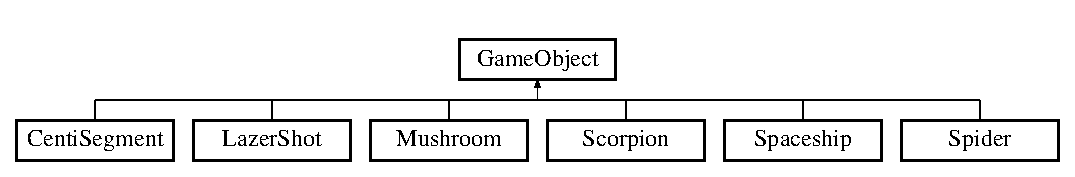
\includegraphics[height=1.924399cm]{class_game_object}
\end{center}
\end{figure}
\subsection*{Public Member Functions}
\begin{DoxyCompactItemize}
\item 
\mbox{\hyperlink{class_game_object_aeff3db3107cbe82af96169ed5b69c09e}{Game\+Object}} (const \mbox{\hyperlink{classvector2_d}{vector2D}} \&size, const \mbox{\hyperlink{classvector2_d}{vector2D}} \&position, float speed, Object\+ID objectid)
\begin{DoxyCompactList}\small\item\em Ensures the creation of a Game\+Objec. \end{DoxyCompactList}\item 
void \mbox{\hyperlink{class_game_object_aa8b57a053c1fee8d3d14912dd9e320c8}{set\+Position}} (const \mbox{\hyperlink{classvector2_d}{vector2D}} \&position)
\begin{DoxyCompactList}\small\item\em set Position of object in the Game \end{DoxyCompactList}\item 
void \mbox{\hyperlink{class_game_object_aeb29555a9bb5cebab57da1960a5085f1}{set\+Size}} (const \mbox{\hyperlink{classvector2_d}{vector2D}} \&size)
\begin{DoxyCompactList}\small\item\em set the size of the object \end{DoxyCompactList}\item 
void \mbox{\hyperlink{class_game_object_a80309e81b799b423a25e180044207114}{set\+Speed}} (float speed)
\begin{DoxyCompactList}\small\item\em set moving speed of the object \end{DoxyCompactList}\item 
void \mbox{\hyperlink{class_game_object_a2ba7a56d4fa8a002fb150989287d6b43}{set\+Object\+ID}} (Object\+ID o\+ID)
\begin{DoxyCompactList}\small\item\em set the object ID \end{DoxyCompactList}\item 
void \mbox{\hyperlink{class_game_object_a77c7875aa47e873967324113060ed2e9}{update\+State}} (State state)
\begin{DoxyCompactList}\small\item\em Indicate current state of object in the game(dead or alive?) \end{DoxyCompactList}\item 
\mbox{\Hypertarget{class_game_object_a4bc279e0b3da8273e4e869cc7584847d}\label{class_game_object_a4bc279e0b3da8273e4e869cc7584847d}} 
virtual void \mbox{\hyperlink{class_game_object_a4bc279e0b3da8273e4e869cc7584847d}{Move}} ()=0
\begin{DoxyCompactList}\small\item\em Move the object in the window. \end{DoxyCompactList}\item 
bool \mbox{\hyperlink{class_game_object_a4a33322fbd4fe9d0d99b56ce872f7d4b}{is\+Dead}} () const
\begin{DoxyCompactList}\small\item\em Check the existance of the object in the Game. \end{DoxyCompactList}\item 
float \mbox{\hyperlink{class_game_object_a70800bd43cf0b786bf6d0f172072b682}{get\+Speed}} () const
\begin{DoxyCompactList}\small\item\em Get speed of the object. \end{DoxyCompactList}\item 
\mbox{\hyperlink{classvector2_d}{vector2D}} \mbox{\hyperlink{class_game_object_a384f1b162b685cbeb8f0c70c03392664}{get\+Position}} () const
\begin{DoxyCompactList}\small\item\em Get position of the object. \end{DoxyCompactList}\item 
\mbox{\hyperlink{classvector2_d}{vector2D}} \mbox{\hyperlink{class_game_object_a2df595e48b25e0377757471f75d89e15}{get\+Size}} () const
\begin{DoxyCompactList}\small\item\em Get size of the object. \end{DoxyCompactList}\item 
Object\+ID \mbox{\hyperlink{class_game_object_a0c8139d67c763ff80cd384000b908a36}{ID}} () const
\begin{DoxyCompactList}\small\item\em get ID of the object \end{DoxyCompactList}\item 
\mbox{\Hypertarget{class_game_object_a3d1fb8fcc7bf0c07b4e619d7dec56b56}\label{class_game_object_a3d1fb8fcc7bf0c07b4e619d7dec56b56}} 
virtual void \mbox{\hyperlink{class_game_object_a3d1fb8fcc7bf0c07b4e619d7dec56b56}{reset}} ()=0
\begin{DoxyCompactList}\small\item\em Reset object to inital conditions. \end{DoxyCompactList}\item 
\mbox{\Hypertarget{class_game_object_aafcceed70da5ea5971b82843ea9222e9}\label{class_game_object_aafcceed70da5ea5971b82843ea9222e9}} 
virtual void \mbox{\hyperlink{class_game_object_aafcceed70da5ea5971b82843ea9222e9}{collision\+Response}} ()=0
\begin{DoxyCompactList}\small\item\em Action taken on collision. \end{DoxyCompactList}\item 
\mbox{\Hypertarget{class_game_object_a224d4f6d9dd75c8a6f9d022eaf586fd9}\label{class_game_object_a224d4f6d9dd75c8a6f9d022eaf586fd9}} 
virtual \mbox{\hyperlink{class_game_object_a224d4f6d9dd75c8a6f9d022eaf586fd9}{$\sim$\+Game\+Object}} ()
\begin{DoxyCompactList}\small\item\em destroy game object \end{DoxyCompactList}\end{DoxyCompactItemize}
\subsection*{Private Attributes}
\begin{DoxyCompactItemize}
\item 
\mbox{\Hypertarget{class_game_object_acf579a65776c0c65955ee6049046c97c}\label{class_game_object_acf579a65776c0c65955ee6049046c97c}} 
\mbox{\hyperlink{classvector2_d}{vector2D}} {\bfseries size\+\_\+}
\item 
\mbox{\Hypertarget{class_game_object_a31345500e5c1c68ffd86565e04d698f9}\label{class_game_object_a31345500e5c1c68ffd86565e04d698f9}} 
\mbox{\hyperlink{classvector2_d}{vector2D}} {\bfseries position\+\_\+}
\item 
\mbox{\Hypertarget{class_game_object_a4ac0cfeb4b4fb47f7069f737d24a8de6}\label{class_game_object_a4ac0cfeb4b4fb47f7069f737d24a8de6}} 
float {\bfseries speed\+\_\+}
\item 
\mbox{\Hypertarget{class_game_object_a3eb63952725ada8dc08282c52a6beb04}\label{class_game_object_a3eb63952725ada8dc08282c52a6beb04}} 
Object\+ID {\bfseries object\+I\+D\+\_\+}
\item 
\mbox{\Hypertarget{class_game_object_a09d2296a020d75e0ffaceee9768405f5}\label{class_game_object_a09d2296a020d75e0ffaceee9768405f5}} 
bool {\bfseries is\+Dead\+\_\+}
\end{DoxyCompactItemize}


\subsection{Detailed Description}
\begin{DoxyAuthor}{Author}
bvrad 
\end{DoxyAuthor}
\begin{DoxyDate}{Date}
08/10/2018 
\end{DoxyDate}


\subsection{Constructor \& Destructor Documentation}
\mbox{\Hypertarget{class_game_object_aeff3db3107cbe82af96169ed5b69c09e}\label{class_game_object_aeff3db3107cbe82af96169ed5b69c09e}} 
\index{Game\+Object@{Game\+Object}!Game\+Object@{Game\+Object}}
\index{Game\+Object@{Game\+Object}!Game\+Object@{Game\+Object}}
\subsubsection{\texorpdfstring{Game\+Object()}{GameObject()}}
{\footnotesize\ttfamily Game\+Object\+::\+Game\+Object (\begin{DoxyParamCaption}\item[{const \mbox{\hyperlink{classvector2_d}{vector2D}} \&}]{size,  }\item[{const \mbox{\hyperlink{classvector2_d}{vector2D}} \&}]{position,  }\item[{float}]{speed,  }\item[{Object\+ID}]{objectid }\end{DoxyParamCaption})}



Ensures the creation of a Game\+Objec. 


\begin{DoxyParams}{Parameters}
{\em position} & \\
\hline
\end{DoxyParams}


\subsection{Member Function Documentation}
\mbox{\Hypertarget{class_game_object_a384f1b162b685cbeb8f0c70c03392664}\label{class_game_object_a384f1b162b685cbeb8f0c70c03392664}} 
\index{Game\+Object@{Game\+Object}!get\+Position@{get\+Position}}
\index{get\+Position@{get\+Position}!Game\+Object@{Game\+Object}}
\subsubsection{\texorpdfstring{get\+Position()}{getPosition()}}
{\footnotesize\ttfamily \mbox{\hyperlink{classvector2_d}{vector2D}} Game\+Object\+::get\+Position (\begin{DoxyParamCaption}{ }\end{DoxyParamCaption}) const\hspace{0.3cm}{\ttfamily [inline]}}



Get position of the object. 

\begin{DoxyReturn}{Returns}
position of the \mbox{\hyperlink{class_game_object}{Game\+Object}} 
\end{DoxyReturn}
\mbox{\Hypertarget{class_game_object_a2df595e48b25e0377757471f75d89e15}\label{class_game_object_a2df595e48b25e0377757471f75d89e15}} 
\index{Game\+Object@{Game\+Object}!get\+Size@{get\+Size}}
\index{get\+Size@{get\+Size}!Game\+Object@{Game\+Object}}
\subsubsection{\texorpdfstring{get\+Size()}{getSize()}}
{\footnotesize\ttfamily \mbox{\hyperlink{classvector2_d}{vector2D}} Game\+Object\+::get\+Size (\begin{DoxyParamCaption}{ }\end{DoxyParamCaption}) const\hspace{0.3cm}{\ttfamily [inline]}}



Get size of the object. 

\begin{DoxyReturn}{Returns}
size of object 
\end{DoxyReturn}
\mbox{\Hypertarget{class_game_object_a70800bd43cf0b786bf6d0f172072b682}\label{class_game_object_a70800bd43cf0b786bf6d0f172072b682}} 
\index{Game\+Object@{Game\+Object}!get\+Speed@{get\+Speed}}
\index{get\+Speed@{get\+Speed}!Game\+Object@{Game\+Object}}
\subsubsection{\texorpdfstring{get\+Speed()}{getSpeed()}}
{\footnotesize\ttfamily float Game\+Object\+::get\+Speed (\begin{DoxyParamCaption}{ }\end{DoxyParamCaption}) const\hspace{0.3cm}{\ttfamily [inline]}}



Get speed of the object. 

\begin{DoxyReturn}{Returns}
speed of the object 
\end{DoxyReturn}
\mbox{\Hypertarget{class_game_object_a0c8139d67c763ff80cd384000b908a36}\label{class_game_object_a0c8139d67c763ff80cd384000b908a36}} 
\index{Game\+Object@{Game\+Object}!ID@{ID}}
\index{ID@{ID}!Game\+Object@{Game\+Object}}
\subsubsection{\texorpdfstring{I\+D()}{ID()}}
{\footnotesize\ttfamily Object\+ID Game\+Object\+::\+ID (\begin{DoxyParamCaption}{ }\end{DoxyParamCaption}) const\hspace{0.3cm}{\ttfamily [inline]}}



get ID of the object 

\begin{DoxyReturn}{Returns}
ID of the object 
\end{DoxyReturn}
\mbox{\Hypertarget{class_game_object_a4a33322fbd4fe9d0d99b56ce872f7d4b}\label{class_game_object_a4a33322fbd4fe9d0d99b56ce872f7d4b}} 
\index{Game\+Object@{Game\+Object}!is\+Dead@{is\+Dead}}
\index{is\+Dead@{is\+Dead}!Game\+Object@{Game\+Object}}
\subsubsection{\texorpdfstring{is\+Dead()}{isDead()}}
{\footnotesize\ttfamily bool Game\+Object\+::is\+Dead (\begin{DoxyParamCaption}{ }\end{DoxyParamCaption}) const\hspace{0.3cm}{\ttfamily [inline]}}



Check the existance of the object in the Game. 

\begin{DoxyReturn}{Returns}
boolean is\+Dead 
\end{DoxyReturn}
\mbox{\Hypertarget{class_game_object_a2ba7a56d4fa8a002fb150989287d6b43}\label{class_game_object_a2ba7a56d4fa8a002fb150989287d6b43}} 
\index{Game\+Object@{Game\+Object}!set\+Object\+ID@{set\+Object\+ID}}
\index{set\+Object\+ID@{set\+Object\+ID}!Game\+Object@{Game\+Object}}
\subsubsection{\texorpdfstring{set\+Object\+I\+D()}{setObjectID()}}
{\footnotesize\ttfamily void Game\+Object\+::set\+Object\+ID (\begin{DoxyParamCaption}\item[{Object\+ID}]{o\+ID }\end{DoxyParamCaption})\hspace{0.3cm}{\ttfamily [inline]}}



set the object ID 


\begin{DoxyParams}{Parameters}
{\em o\+ID} & ID of the Object \\
\hline
\end{DoxyParams}
\mbox{\Hypertarget{class_game_object_aa8b57a053c1fee8d3d14912dd9e320c8}\label{class_game_object_aa8b57a053c1fee8d3d14912dd9e320c8}} 
\index{Game\+Object@{Game\+Object}!set\+Position@{set\+Position}}
\index{set\+Position@{set\+Position}!Game\+Object@{Game\+Object}}
\subsubsection{\texorpdfstring{set\+Position()}{setPosition()}}
{\footnotesize\ttfamily void Game\+Object\+::set\+Position (\begin{DoxyParamCaption}\item[{const \mbox{\hyperlink{classvector2_d}{vector2D}} \&}]{position }\end{DoxyParamCaption})}



set Position of object in the Game 


\begin{DoxyParams}{Parameters}
{\em position} & of the object \\
\hline
\end{DoxyParams}
\mbox{\Hypertarget{class_game_object_aeb29555a9bb5cebab57da1960a5085f1}\label{class_game_object_aeb29555a9bb5cebab57da1960a5085f1}} 
\index{Game\+Object@{Game\+Object}!set\+Size@{set\+Size}}
\index{set\+Size@{set\+Size}!Game\+Object@{Game\+Object}}
\subsubsection{\texorpdfstring{set\+Size()}{setSize()}}
{\footnotesize\ttfamily void Game\+Object\+::set\+Size (\begin{DoxyParamCaption}\item[{const \mbox{\hyperlink{classvector2_d}{vector2D}} \&}]{size }\end{DoxyParamCaption})\hspace{0.3cm}{\ttfamily [inline]}}



set the size of the object 


\begin{DoxyParams}{Parameters}
{\em size} & of the \mbox{\hyperlink{class_game_object}{Game\+Object}} \\
\hline
\end{DoxyParams}
\mbox{\Hypertarget{class_game_object_a80309e81b799b423a25e180044207114}\label{class_game_object_a80309e81b799b423a25e180044207114}} 
\index{Game\+Object@{Game\+Object}!set\+Speed@{set\+Speed}}
\index{set\+Speed@{set\+Speed}!Game\+Object@{Game\+Object}}
\subsubsection{\texorpdfstring{set\+Speed()}{setSpeed()}}
{\footnotesize\ttfamily void Game\+Object\+::set\+Speed (\begin{DoxyParamCaption}\item[{float}]{speed }\end{DoxyParamCaption})\hspace{0.3cm}{\ttfamily [inline]}}



set moving speed of the object 


\begin{DoxyParams}{Parameters}
{\em speed} & of the \mbox{\hyperlink{class_game_object}{Game\+Object}} \\
\hline
\end{DoxyParams}
\mbox{\Hypertarget{class_game_object_a77c7875aa47e873967324113060ed2e9}\label{class_game_object_a77c7875aa47e873967324113060ed2e9}} 
\index{Game\+Object@{Game\+Object}!update\+State@{update\+State}}
\index{update\+State@{update\+State}!Game\+Object@{Game\+Object}}
\subsubsection{\texorpdfstring{update\+State()}{updateState()}}
{\footnotesize\ttfamily void Game\+Object\+::update\+State (\begin{DoxyParamCaption}\item[{State}]{state }\end{DoxyParamCaption})}



Indicate current state of object in the game(dead or alive?) 


\begin{DoxyParams}{Parameters}
{\em state} & of the \mbox{\hyperlink{class_game_object}{Game\+Object}} \\
\hline
\end{DoxyParams}


The documentation for this class was generated from the following files\+:\begin{DoxyCompactItemize}
\item 
C\+:/\+Users/bvrad/\+Dropbox/\+Boikanyo/elen3009/\+P\+R\+O\+J\+E\+C\+T/2018-\/project-\/1386807-\/\+Radiokana-\/1427726-\/\+Sepuru/game-\/source-\/code/\mbox{\hyperlink{_game_object_8h}{Game\+Object.\+h}}\item 
C\+:/\+Users/bvrad/\+Dropbox/\+Boikanyo/elen3009/\+P\+R\+O\+J\+E\+C\+T/2018-\/project-\/1386807-\/\+Radiokana-\/1427726-\/\+Sepuru/game-\/source-\/code/Game\+Object.\+cpp\end{DoxyCompactItemize}

\hypertarget{class_game_object_container}{}\section{Game\+Object\+Container Class Reference}
\label{class_game_object_container}\index{Game\+Object\+Container@{Game\+Object\+Container}}


{\ttfamily \#include $<$Game\+Object\+Container.\+h$>$}

Inheritance diagram for Game\+Object\+Container\+:\begin{figure}[H]
\begin{center}
\leavevmode
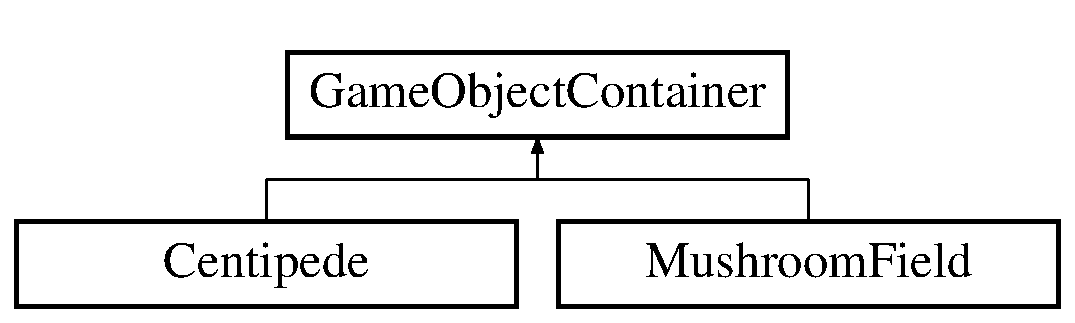
\includegraphics[height=2.000000cm]{class_game_object_container}
\end{center}
\end{figure}
\subsection*{Public Member Functions}
\begin{DoxyCompactItemize}
\item 
\mbox{\hyperlink{class_game_object_container_ad3b33550acd14414d6434e6836885f3c}{Game\+Object\+Container}} (int \mbox{\hyperlink{class_game_object_container_a4502e18e58c774b681e7ef8e6319910d}{size}})
\begin{DoxyCompactList}\small\item\em Constructor. \end{DoxyCompactList}\item 
virtual shared\+\_\+ptr$<$ \mbox{\hyperlink{class_game_object}{Game\+Object}} $>$ \mbox{\hyperlink{class_game_object_container_affa50b43ca7b82d54055b6499e024aba}{segment}} (int i) const =0
\begin{DoxyCompactList}\small\item\em return segment of the game\+Object\+Container \end{DoxyCompactList}\item 
\mbox{\Hypertarget{class_game_object_container_a13ed0612c4c8226f196c9c219f38cb65}\label{class_game_object_container_a13ed0612c4c8226f196c9c219f38cb65}} 
virtual void \mbox{\hyperlink{class_game_object_container_a13ed0612c4c8226f196c9c219f38cb65}{reset}} ()=0
\begin{DoxyCompactList}\small\item\em Resize \mbox{\hyperlink{class_game_object}{Game\+Object}} Container. \end{DoxyCompactList}\item 
void \mbox{\hyperlink{class_game_object_container_a4502e18e58c774b681e7ef8e6319910d}{size}} (int size)
\begin{DoxyCompactList}\small\item\em set size of \mbox{\hyperlink{class_game_object_container}{Game\+Object\+Container}} \end{DoxyCompactList}\item 
int \mbox{\hyperlink{class_game_object_container_afda69d0805c2ee12dd2b972fd66b34c9}{size}} ()
\begin{DoxyCompactList}\small\item\em get size of Game\+Object\+Conatiner \end{DoxyCompactList}\item 
\mbox{\Hypertarget{class_game_object_container_a84e10f78eae954c67c6c0ac30797a8bf}\label{class_game_object_container_a84e10f78eae954c67c6c0ac30797a8bf}} 
virtual \mbox{\hyperlink{class_game_object_container_a84e10f78eae954c67c6c0ac30797a8bf}{$\sim$\+Game\+Object\+Container}} ()
\begin{DoxyCompactList}\small\item\em Destroy the object. \end{DoxyCompactList}\end{DoxyCompactItemize}
\subsection*{Private Attributes}
\begin{DoxyCompactItemize}
\item 
\mbox{\Hypertarget{class_game_object_container_a49c7e858bdedb0c05cbab00d0a0bd46f}\label{class_game_object_container_a49c7e858bdedb0c05cbab00d0a0bd46f}} 
int {\bfseries size\+\_\+}
\end{DoxyCompactItemize}


\subsection{Detailed Description}
\begin{DoxyDate}{Date}
08/10/2018 
\end{DoxyDate}


\subsection{Constructor \& Destructor Documentation}
\mbox{\Hypertarget{class_game_object_container_ad3b33550acd14414d6434e6836885f3c}\label{class_game_object_container_ad3b33550acd14414d6434e6836885f3c}} 
\index{Game\+Object\+Container@{Game\+Object\+Container}!Game\+Object\+Container@{Game\+Object\+Container}}
\index{Game\+Object\+Container@{Game\+Object\+Container}!Game\+Object\+Container@{Game\+Object\+Container}}
\subsubsection{\texorpdfstring{Game\+Object\+Container()}{GameObjectContainer()}}
{\footnotesize\ttfamily Game\+Object\+Container\+::\+Game\+Object\+Container (\begin{DoxyParamCaption}\item[{int}]{size }\end{DoxyParamCaption})\hspace{0.3cm}{\ttfamily [inline]}}



Constructor. 


\begin{DoxyParams}{Parameters}
{\em size} & of the container \\
\hline
\end{DoxyParams}


\subsection{Member Function Documentation}
\mbox{\Hypertarget{class_game_object_container_affa50b43ca7b82d54055b6499e024aba}\label{class_game_object_container_affa50b43ca7b82d54055b6499e024aba}} 
\index{Game\+Object\+Container@{Game\+Object\+Container}!segment@{segment}}
\index{segment@{segment}!Game\+Object\+Container@{Game\+Object\+Container}}
\subsubsection{\texorpdfstring{segment()}{segment()}}
{\footnotesize\ttfamily virtual shared\+\_\+ptr$<$\mbox{\hyperlink{class_game_object}{Game\+Object}}$>$ Game\+Object\+Container\+::segment (\begin{DoxyParamCaption}\item[{int}]{i }\end{DoxyParamCaption}) const\hspace{0.3cm}{\ttfamily [pure virtual]}}



return segment of the game\+Object\+Container 


\begin{DoxyParams}{Parameters}
{\em i} & iterator to container \\
\hline
\end{DoxyParams}
\begin{DoxyReturn}{Returns}
ith segment of the container 
\end{DoxyReturn}


Implemented in \mbox{\hyperlink{class_centipede_ae722488780d0d19e63510647b5fe108c}{Centipede}}, and \mbox{\hyperlink{class_mushroom_field_a478cc3df9deaf0e7a0b48fd2d128eeb8}{Mushroom\+Field}}.

\mbox{\Hypertarget{class_game_object_container_a4502e18e58c774b681e7ef8e6319910d}\label{class_game_object_container_a4502e18e58c774b681e7ef8e6319910d}} 
\index{Game\+Object\+Container@{Game\+Object\+Container}!size@{size}}
\index{size@{size}!Game\+Object\+Container@{Game\+Object\+Container}}
\subsubsection{\texorpdfstring{size()}{size()}\hspace{0.1cm}{\footnotesize\ttfamily [1/2]}}
{\footnotesize\ttfamily void Game\+Object\+Container\+::size (\begin{DoxyParamCaption}\item[{int}]{size }\end{DoxyParamCaption})\hspace{0.3cm}{\ttfamily [inline]}}



set size of \mbox{\hyperlink{class_game_object_container}{Game\+Object\+Container}} 


\begin{DoxyParams}{Parameters}
{\em size} & of the container \\
\hline
\end{DoxyParams}
\mbox{\Hypertarget{class_game_object_container_afda69d0805c2ee12dd2b972fd66b34c9}\label{class_game_object_container_afda69d0805c2ee12dd2b972fd66b34c9}} 
\index{Game\+Object\+Container@{Game\+Object\+Container}!size@{size}}
\index{size@{size}!Game\+Object\+Container@{Game\+Object\+Container}}
\subsubsection{\texorpdfstring{size()}{size()}\hspace{0.1cm}{\footnotesize\ttfamily [2/2]}}
{\footnotesize\ttfamily int Game\+Object\+Container\+::size (\begin{DoxyParamCaption}{ }\end{DoxyParamCaption})\hspace{0.3cm}{\ttfamily [inline]}}



get size of Game\+Object\+Conatiner 

\begin{DoxyReturn}{Returns}
size of the container 
\end{DoxyReturn}


The documentation for this class was generated from the following file\+:\begin{DoxyCompactItemize}
\item 
C\+:/\+Users/bvrad/\+Dropbox/\+Boikanyo/elen3009/\+P\+R\+O\+J\+E\+C\+T/2018-\/project-\/1386807-\/\+Radiokana-\/1427726-\/\+Sepuru/game-\/source-\/code/\mbox{\hyperlink{_game_object_container_8h}{Game\+Object\+Container.\+h}}\end{DoxyCompactItemize}

\hypertarget{class_lazer_shot}{}\section{Lazer\+Shot Class Reference}
\label{class_lazer_shot}\index{Lazer\+Shot@{Lazer\+Shot}}


{\ttfamily \#include $<$Lazer\+Shot.\+h$>$}

Inheritance diagram for Lazer\+Shot\+:\begin{figure}[H]
\begin{center}
\leavevmode
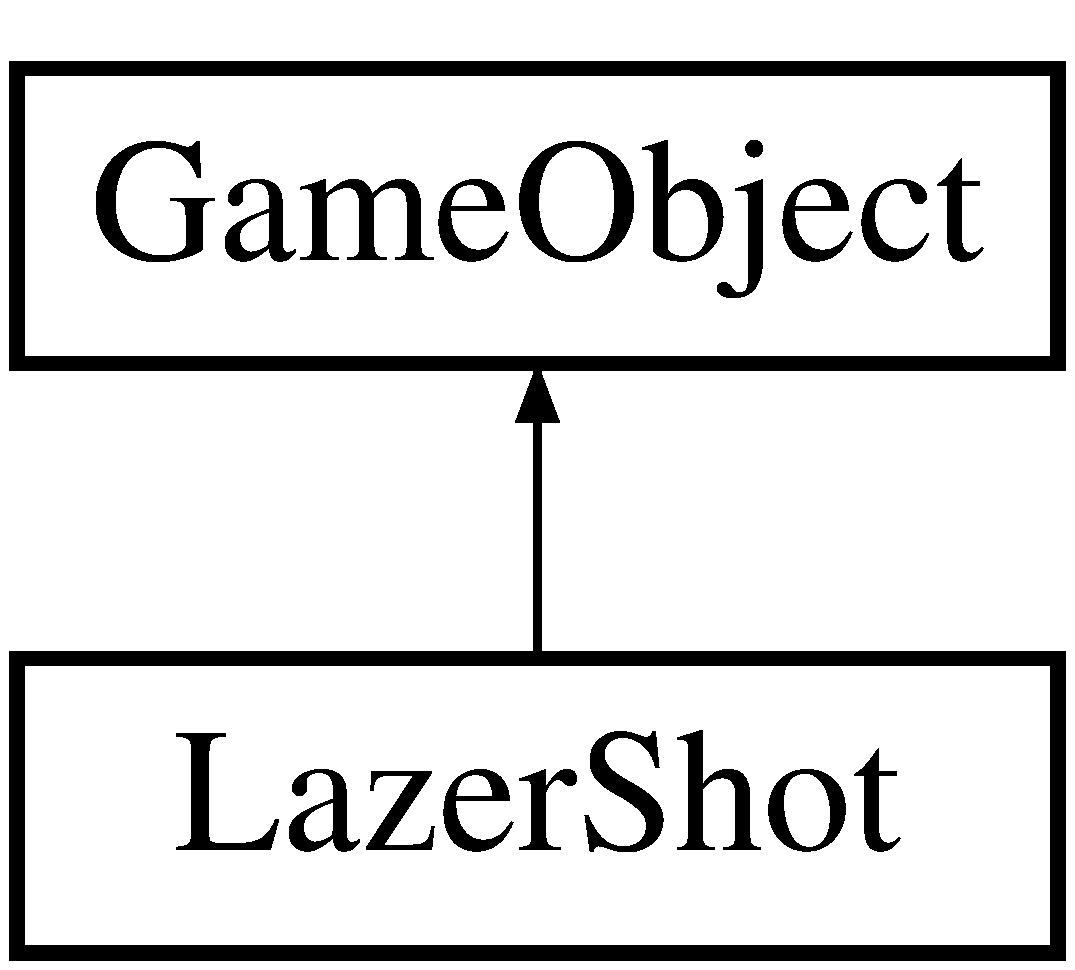
\includegraphics[height=2.000000cm]{class_lazer_shot}
\end{center}
\end{figure}
\subsection*{Public Member Functions}
\begin{DoxyCompactItemize}
\item 
\mbox{\hyperlink{class_lazer_shot_a16416eaac233433aae4e95edb48b129d}{Lazer\+Shot}} (const \mbox{\hyperlink{classvector2_d}{vector2D}} \&size, const \mbox{\hyperlink{classvector2_d}{vector2D}} \&position, float speed, Object\+ID objectid)
\begin{DoxyCompactList}\small\item\em Constructor of the \mbox{\hyperlink{class_lazer_shot}{Lazer\+Shot}} Class. \end{DoxyCompactList}\item 
void \mbox{\hyperlink{class_lazer_shot_a361cd2740db7f69f92a4938c06e5e46c}{Load}} (const \mbox{\hyperlink{classvector2_d}{vector2D}} \&position)
\begin{DoxyCompactList}\small\item\em Load Lazershot to player. \end{DoxyCompactList}\item 
\mbox{\Hypertarget{class_lazer_shot_a7f41ca3cb80b80c1eacea35c2d3f0d61}\label{class_lazer_shot_a7f41ca3cb80b80c1eacea35c2d3f0d61}} 
virtual void \mbox{\hyperlink{class_lazer_shot_a7f41ca3cb80b80c1eacea35c2d3f0d61}{Move}} () override
\begin{DoxyCompactList}\small\item\em move the Lazershot \end{DoxyCompactList}\item 
\mbox{\Hypertarget{class_lazer_shot_aee471cae1fb2ac98db353812d8b4f812}\label{class_lazer_shot_aee471cae1fb2ac98db353812d8b4f812}} 
void \mbox{\hyperlink{class_lazer_shot_aee471cae1fb2ac98db353812d8b4f812}{Fire}} ()
\begin{DoxyCompactList}\small\item\em move the Lazershot \end{DoxyCompactList}\item 
\mbox{\Hypertarget{class_lazer_shot_aa45b3c708990784379403fea5f1c7b1d}\label{class_lazer_shot_aa45b3c708990784379403fea5f1c7b1d}} 
virtual void \mbox{\hyperlink{class_lazer_shot_aa45b3c708990784379403fea5f1c7b1d}{reset}} () override
\begin{DoxyCompactList}\small\item\em destroy Lazershot \end{DoxyCompactList}\item 
\mbox{\Hypertarget{class_lazer_shot_a890ffaf8ff5af439e67c33805f7a7b06}\label{class_lazer_shot_a890ffaf8ff5af439e67c33805f7a7b06}} 
virtual void \mbox{\hyperlink{class_lazer_shot_a890ffaf8ff5af439e67c33805f7a7b06}{collision\+Response}} () override
\begin{DoxyCompactList}\small\item\em \mbox{\hyperlink{class_collision}{Collision}} response of Lazer\+Shoot. \end{DoxyCompactList}\item 
\mbox{\Hypertarget{class_lazer_shot_a67497615bb40710e312817d500f78b1e}\label{class_lazer_shot_a67497615bb40710e312817d500f78b1e}} 
virtual \mbox{\hyperlink{class_lazer_shot_a67497615bb40710e312817d500f78b1e}{$\sim$\+Lazer\+Shot}} ()
\begin{DoxyCompactList}\small\item\em Destroy \mbox{\hyperlink{class_lazer_shot}{Lazer\+Shot}}. \end{DoxyCompactList}\end{DoxyCompactItemize}


\subsection{Detailed Description}
\begin{DoxyDate}{Date}
08/10/2018 
\end{DoxyDate}


\subsection{Constructor \& Destructor Documentation}
\mbox{\Hypertarget{class_lazer_shot_a16416eaac233433aae4e95edb48b129d}\label{class_lazer_shot_a16416eaac233433aae4e95edb48b129d}} 
\index{Lazer\+Shot@{Lazer\+Shot}!Lazer\+Shot@{Lazer\+Shot}}
\index{Lazer\+Shot@{Lazer\+Shot}!Lazer\+Shot@{Lazer\+Shot}}
\subsubsection{\texorpdfstring{Lazer\+Shot()}{LazerShot()}}
{\footnotesize\ttfamily Lazer\+Shot\+::\+Lazer\+Shot (\begin{DoxyParamCaption}\item[{const \mbox{\hyperlink{classvector2_d}{vector2D}} \&}]{size,  }\item[{const \mbox{\hyperlink{classvector2_d}{vector2D}} \&}]{position,  }\item[{float}]{speed,  }\item[{Object\+ID}]{objectid }\end{DoxyParamCaption})\hspace{0.3cm}{\ttfamily [inline]}}



Constructor of the \mbox{\hyperlink{class_lazer_shot}{Lazer\+Shot}} Class. 


\begin{DoxyParams}{Parameters}
{\em size} & of the Lazer\+Shots \\
\hline
{\em position} & of the \mbox{\hyperlink{class_lazer_shot}{Lazer\+Shot}} \\
\hline
{\em speed} & of the \mbox{\hyperlink{class_lazer_shot}{Lazer\+Shot}} \\
\hline
{\em objectid} & ID of the \mbox{\hyperlink{class_lazer_shot}{Lazer\+Shot}} \\
\hline
\end{DoxyParams}


\subsection{Member Function Documentation}
\mbox{\Hypertarget{class_lazer_shot_a361cd2740db7f69f92a4938c06e5e46c}\label{class_lazer_shot_a361cd2740db7f69f92a4938c06e5e46c}} 
\index{Lazer\+Shot@{Lazer\+Shot}!Load@{Load}}
\index{Load@{Load}!Lazer\+Shot@{Lazer\+Shot}}
\subsubsection{\texorpdfstring{Load()}{Load()}}
{\footnotesize\ttfamily void Lazer\+Shot\+::\+Load (\begin{DoxyParamCaption}\item[{const \mbox{\hyperlink{classvector2_d}{vector2D}} \&}]{position }\end{DoxyParamCaption})\hspace{0.3cm}{\ttfamily [inline]}}



Load Lazershot to player. 


\begin{DoxyParams}{Parameters}
{\em position} & of the \mbox{\hyperlink{class_player}{Player}} \\
\hline
\end{DoxyParams}


The documentation for this class was generated from the following files\+:\begin{DoxyCompactItemize}
\item 
C\+:/\+Users/bvrad/\+Dropbox/\+Boikanyo/elen3009/\+P\+R\+O\+J\+E\+C\+T/2018-\/project-\/1386807-\/\+Radiokana-\/1427726-\/\+Sepuru/game-\/source-\/code/\mbox{\hyperlink{_lazer_shot_8h}{Lazer\+Shot.\+h}}\item 
C\+:/\+Users/bvrad/\+Dropbox/\+Boikanyo/elen3009/\+P\+R\+O\+J\+E\+C\+T/2018-\/project-\/1386807-\/\+Radiokana-\/1427726-\/\+Sepuru/game-\/source-\/code/Lazer\+Shot.\+cpp\end{DoxyCompactItemize}

\hypertarget{class_mushroom}{}\section{Mushroom Class Reference}
\label{class_mushroom}\index{Mushroom@{Mushroom}}


{\ttfamily \#include $<$Mushroom.\+h$>$}

Inheritance diagram for Mushroom\+:\begin{figure}[H]
\begin{center}
\leavevmode
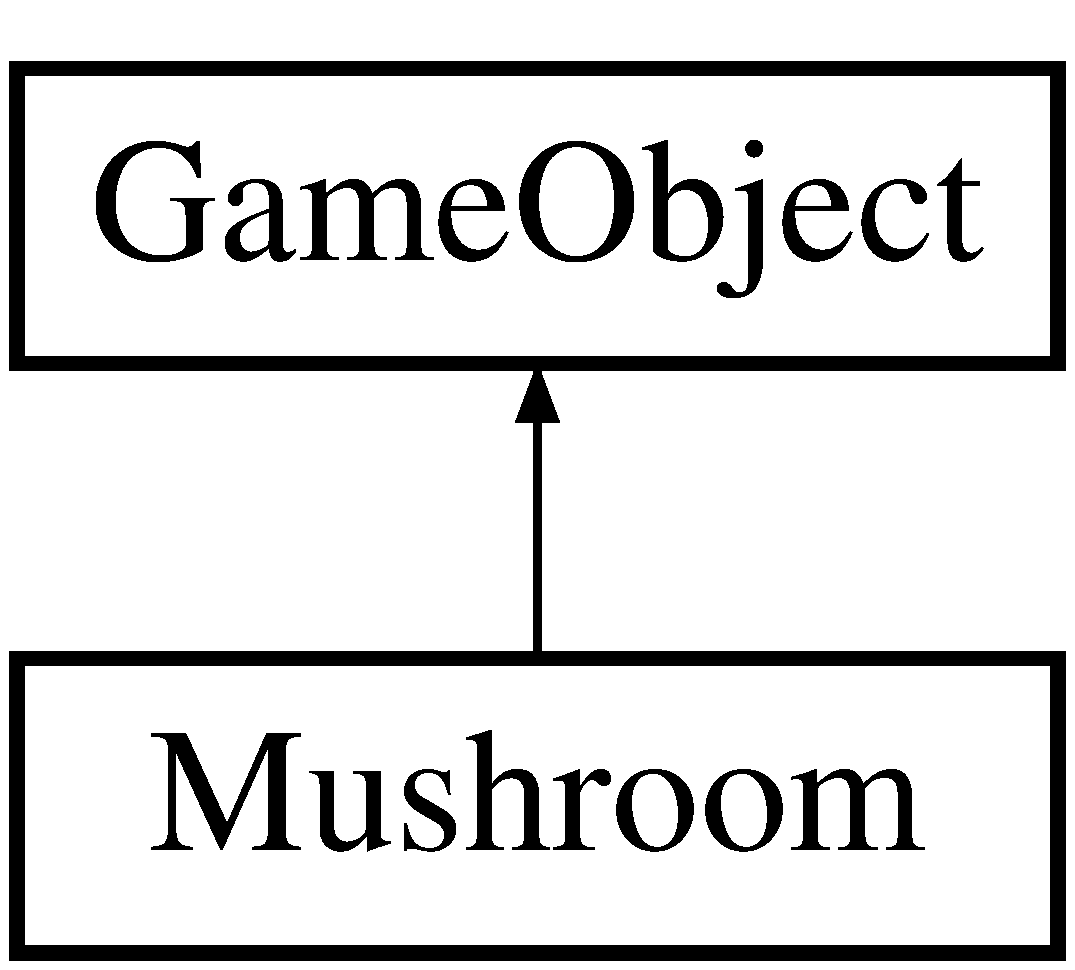
\includegraphics[height=2.000000cm]{class_mushroom}
\end{center}
\end{figure}
\subsection*{Public Member Functions}
\begin{DoxyCompactItemize}
\item 
\mbox{\hyperlink{class_mushroom_afa955bb8eaaddc45571725b3e04c4c09}{Mushroom}} (const \mbox{\hyperlink{classvector2_d}{vector2D}} \&size, const \mbox{\hyperlink{classvector2_d}{vector2D}} \&position, float speed, Object\+ID objectid)
\begin{DoxyCompactList}\small\item\em Constructor of the \mbox{\hyperlink{class_mushroom}{Mushroom}} Class. \end{DoxyCompactList}\item 
\mbox{\Hypertarget{class_mushroom_aa8d02f56dc9de6e73f61f8b68f8db5da}\label{class_mushroom_aa8d02f56dc9de6e73f61f8b68f8db5da}} 
virtual void \mbox{\hyperlink{class_mushroom_aa8d02f56dc9de6e73f61f8b68f8db5da}{collision\+Response}} () override
\begin{DoxyCompactList}\small\item\em Take action if \mbox{\hyperlink{class_mushroom}{Mushroom}} is shot. \end{DoxyCompactList}\item 
int \mbox{\hyperlink{class_mushroom_afe84a485e2eb67e1efadd49ef77cb79e}{lives}} () const
\begin{DoxyCompactList}\small\item\em Return the number of lives the \mbox{\hyperlink{class_mushroom}{Mushroom}} has. \end{DoxyCompactList}\item 
\mbox{\Hypertarget{class_mushroom_a83ecffb484e4c3931e3dbd7eaa085e59}\label{class_mushroom_a83ecffb484e4c3931e3dbd7eaa085e59}} 
virtual void \mbox{\hyperlink{class_mushroom_a83ecffb484e4c3931e3dbd7eaa085e59}{Move}} () override
\begin{DoxyCompactList}\small\item\em Move function from parent. \end{DoxyCompactList}\item 
\mbox{\Hypertarget{class_mushroom_a9801ad2b960bee6bf66851434ba64b21}\label{class_mushroom_a9801ad2b960bee6bf66851434ba64b21}} 
virtual void \mbox{\hyperlink{class_mushroom_a9801ad2b960bee6bf66851434ba64b21}{reset}} () override
\begin{DoxyCompactList}\small\item\em Reset \mbox{\hyperlink{class_mushroom}{Mushroom}} to intial conditions. \end{DoxyCompactList}\item 
\mbox{\Hypertarget{class_mushroom_a0cf0e035c2fcc711a4ae378eafa59fab}\label{class_mushroom_a0cf0e035c2fcc711a4ae378eafa59fab}} 
virtual \mbox{\hyperlink{class_mushroom_a0cf0e035c2fcc711a4ae378eafa59fab}{$\sim$\+Mushroom}} ()
\begin{DoxyCompactList}\small\item\em Destroy \mbox{\hyperlink{class_mushroom}{Mushroom}} Object. \end{DoxyCompactList}\end{DoxyCompactItemize}
\subsection*{Private Attributes}
\begin{DoxyCompactItemize}
\item 
\mbox{\Hypertarget{class_mushroom_a4fb3b9d849a6c27234b998685da2dad1}\label{class_mushroom_a4fb3b9d849a6c27234b998685da2dad1}} 
int {\bfseries lives\+\_\+} = 4
\end{DoxyCompactItemize}


\subsection{Detailed Description}
\begin{DoxyDate}{Date}
08/10/2018 
\end{DoxyDate}


\subsection{Constructor \& Destructor Documentation}
\mbox{\Hypertarget{class_mushroom_afa955bb8eaaddc45571725b3e04c4c09}\label{class_mushroom_afa955bb8eaaddc45571725b3e04c4c09}} 
\index{Mushroom@{Mushroom}!Mushroom@{Mushroom}}
\index{Mushroom@{Mushroom}!Mushroom@{Mushroom}}
\subsubsection{\texorpdfstring{Mushroom()}{Mushroom()}}
{\footnotesize\ttfamily Mushroom\+::\+Mushroom (\begin{DoxyParamCaption}\item[{const \mbox{\hyperlink{classvector2_d}{vector2D}} \&}]{size,  }\item[{const \mbox{\hyperlink{classvector2_d}{vector2D}} \&}]{position,  }\item[{float}]{speed,  }\item[{Object\+ID}]{objectid }\end{DoxyParamCaption})\hspace{0.3cm}{\ttfamily [inline]}}



Constructor of the \mbox{\hyperlink{class_mushroom}{Mushroom}} Class. 


\begin{DoxyParams}{Parameters}
{\em size} & of the \mbox{\hyperlink{class_mushroom}{Mushroom}} \\
\hline
{\em position} & of the \mbox{\hyperlink{class_mushroom}{Mushroom}} \\
\hline
{\em speed} & of the \mbox{\hyperlink{class_mushroom}{Mushroom}} \\
\hline
{\em objectid} & ID of the \mbox{\hyperlink{class_mushroom}{Mushroom}} \\
\hline
\end{DoxyParams}


\subsection{Member Function Documentation}
\mbox{\Hypertarget{class_mushroom_afe84a485e2eb67e1efadd49ef77cb79e}\label{class_mushroom_afe84a485e2eb67e1efadd49ef77cb79e}} 
\index{Mushroom@{Mushroom}!lives@{lives}}
\index{lives@{lives}!Mushroom@{Mushroom}}
\subsubsection{\texorpdfstring{lives()}{lives()}}
{\footnotesize\ttfamily int Mushroom\+::lives (\begin{DoxyParamCaption}{ }\end{DoxyParamCaption}) const\hspace{0.3cm}{\ttfamily [inline]}}



Return the number of lives the \mbox{\hyperlink{class_mushroom}{Mushroom}} has. 

\begin{DoxyReturn}{Returns}
number of lives 
\end{DoxyReturn}


The documentation for this class was generated from the following files\+:\begin{DoxyCompactItemize}
\item 
C\+:/\+Users/bvrad/\+Dropbox/\+Boikanyo/elen3009/\+P\+R\+O\+J\+E\+C\+T/2018-\/project-\/1386807-\/\+Radiokana-\/1427726-\/\+Sepuru/game-\/source-\/code/\mbox{\hyperlink{_mushroom_8h}{Mushroom.\+h}}\item 
C\+:/\+Users/bvrad/\+Dropbox/\+Boikanyo/elen3009/\+P\+R\+O\+J\+E\+C\+T/2018-\/project-\/1386807-\/\+Radiokana-\/1427726-\/\+Sepuru/game-\/source-\/code/Mushroom.\+cpp\end{DoxyCompactItemize}

\hypertarget{class_mushroom_field}{}\section{Mushroom\+Field Class Reference}
\label{class_mushroom_field}\index{Mushroom\+Field@{Mushroom\+Field}}


{\ttfamily \#include $<$Mushroom\+Field.\+h$>$}

Inheritance diagram for Mushroom\+Field\+:\begin{figure}[H]
\begin{center}
\leavevmode
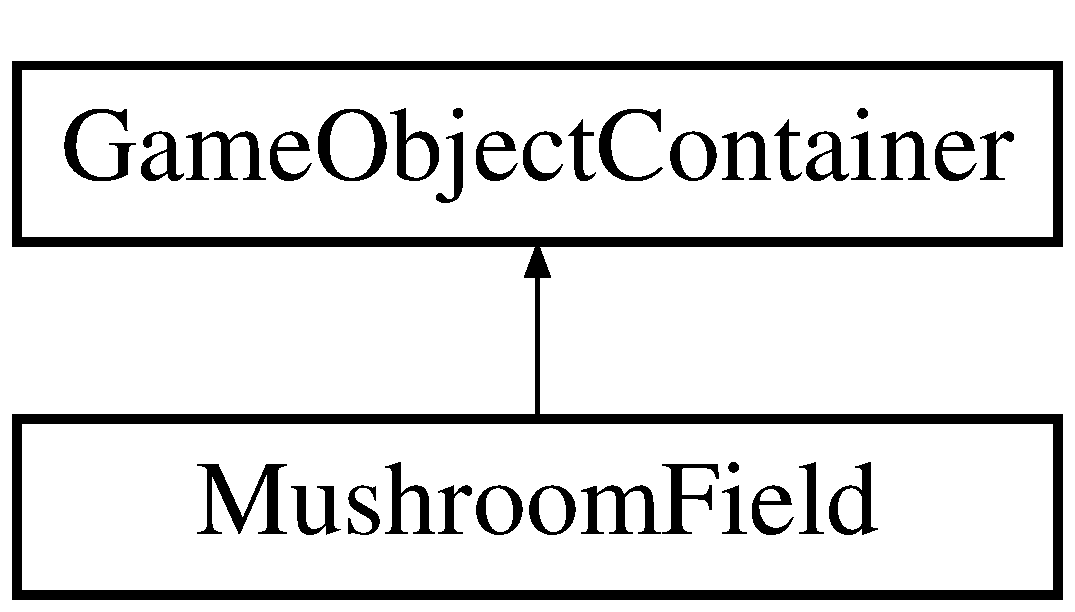
\includegraphics[height=2.000000cm]{class_mushroom_field}
\end{center}
\end{figure}
\subsection*{Public Member Functions}
\begin{DoxyCompactItemize}
\item 
\mbox{\hyperlink{class_mushroom_field_af2fe64e9f63e8fcec6a5bbae644de4cb}{Mushroom\+Field}} (int \mbox{\hyperlink{class_game_object_container_a4502e18e58c774b681e7ef8e6319910d}{size}})
\begin{DoxyCompactList}\small\item\em Constructor. \end{DoxyCompactList}\item 
virtual shared\+\_\+ptr$<$ \mbox{\hyperlink{class_game_object}{Game\+Object}} $>$ \mbox{\hyperlink{class_mushroom_field_a478cc3df9deaf0e7a0b48fd2d128eeb8}{segment}} (int i) const override
\begin{DoxyCompactList}\small\item\em Return a \mbox{\hyperlink{class_mushroom}{Mushroom}} at index i. \end{DoxyCompactList}\item 
void \mbox{\hyperlink{class_mushroom_field_aa182f3e0d33fccac34c7237e7994ecb7}{transform}} (std\+::shared\+\_\+ptr$<$ \mbox{\hyperlink{class_game_object}{Game\+Object}} $>$ centi\+Seg\+\_\+ptr)
\begin{DoxyCompactList}\small\item\em Transform centipe segment to \mbox{\hyperlink{class_mushroom}{Mushroom}}. \end{DoxyCompactList}\item 
\mbox{\Hypertarget{class_mushroom_field_a244cff4ad63184c6c41e1e4bac007a2a}\label{class_mushroom_field_a244cff4ad63184c6c41e1e4bac007a2a}} 
virtual void \mbox{\hyperlink{class_mushroom_field_a244cff4ad63184c6c41e1e4bac007a2a}{reset}} () override
\begin{DoxyCompactList}\small\item\em Regenerate field. \end{DoxyCompactList}\item 
\mbox{\Hypertarget{class_mushroom_field_ac3918d58b61d0f51e851cb02964f0d73}\label{class_mushroom_field_ac3918d58b61d0f51e851cb02964f0d73}} 
virtual \mbox{\hyperlink{class_mushroom_field_ac3918d58b61d0f51e851cb02964f0d73}{$\sim$\+Mushroom\+Field}} ()
\begin{DoxyCompactList}\small\item\em Destroy the \mbox{\hyperlink{class_mushroom_field}{Mushroom\+Field}} Object. \end{DoxyCompactList}\end{DoxyCompactItemize}
\subsection*{Private Member Functions}
\begin{DoxyCompactItemize}
\item 
\mbox{\Hypertarget{class_mushroom_field_a18609a3ce909bc03f9d5b04a166e80ab}\label{class_mushroom_field_a18609a3ce909bc03f9d5b04a166e80ab}} 
void \mbox{\hyperlink{class_mushroom_field_a18609a3ce909bc03f9d5b04a166e80ab}{generate\+Field}} ()
\begin{DoxyCompactList}\small\item\em Generate random field of Mushrooms. \end{DoxyCompactList}\end{DoxyCompactItemize}
\subsection*{Private Attributes}
\begin{DoxyCompactItemize}
\item 
\mbox{\Hypertarget{class_mushroom_field_a8fc5cfef80a4e3e738179f6314603d8d}\label{class_mushroom_field_a8fc5cfef80a4e3e738179f6314603d8d}} 
int {\bfseries original\+\_\+size\+\_\+}
\item 
\mbox{\Hypertarget{class_mushroom_field_a15e1b4da78b48430eb6e59003af6446e}\label{class_mushroom_field_a15e1b4da78b48430eb6e59003af6446e}} 
vector$<$ shared\+\_\+ptr$<$ \mbox{\hyperlink{class_mushroom}{Mushroom}} $>$ $>$ {\bfseries \+\_\+mushrooms\+\_\+ptr}
\item 
\mbox{\Hypertarget{class_mushroom_field_ae5604bf107ab35250250148c6a5cb378}\label{class_mushroom_field_ae5604bf107ab35250250148c6a5cb378}} 
vector$<$ float $>$ {\bfseries y\+Positions\+\_\+}
\item 
\mbox{\Hypertarget{class_mushroom_field_a6997a1424b8217d589bca4e605ce5c6a}\label{class_mushroom_field_a6997a1424b8217d589bca4e605ce5c6a}} 
vector$<$ float $>$ {\bfseries x\+Positions\+\_\+}
\end{DoxyCompactItemize}


\subsection{Detailed Description}
\begin{DoxyDate}{Date}
08/10/2018 
\end{DoxyDate}


\subsection{Constructor \& Destructor Documentation}
\mbox{\Hypertarget{class_mushroom_field_af2fe64e9f63e8fcec6a5bbae644de4cb}\label{class_mushroom_field_af2fe64e9f63e8fcec6a5bbae644de4cb}} 
\index{Mushroom\+Field@{Mushroom\+Field}!Mushroom\+Field@{Mushroom\+Field}}
\index{Mushroom\+Field@{Mushroom\+Field}!Mushroom\+Field@{Mushroom\+Field}}
\subsubsection{\texorpdfstring{Mushroom\+Field()}{MushroomField()}}
{\footnotesize\ttfamily Mushroom\+Field\+::\+Mushroom\+Field (\begin{DoxyParamCaption}\item[{int}]{size }\end{DoxyParamCaption})}



Constructor. 


\begin{DoxyParams}{Parameters}
{\em size} & of the \mbox{\hyperlink{class_mushroom_field}{Mushroom\+Field}} \\
\hline
\end{DoxyParams}


\subsection{Member Function Documentation}
\mbox{\Hypertarget{class_mushroom_field_a478cc3df9deaf0e7a0b48fd2d128eeb8}\label{class_mushroom_field_a478cc3df9deaf0e7a0b48fd2d128eeb8}} 
\index{Mushroom\+Field@{Mushroom\+Field}!segment@{segment}}
\index{segment@{segment}!Mushroom\+Field@{Mushroom\+Field}}
\subsubsection{\texorpdfstring{segment()}{segment()}}
{\footnotesize\ttfamily virtual shared\+\_\+ptr$<$\mbox{\hyperlink{class_game_object}{Game\+Object}}$>$ Mushroom\+Field\+::segment (\begin{DoxyParamCaption}\item[{int}]{i }\end{DoxyParamCaption}) const\hspace{0.3cm}{\ttfamily [inline]}, {\ttfamily [override]}, {\ttfamily [virtual]}}



Return a \mbox{\hyperlink{class_mushroom}{Mushroom}} at index i. 


\begin{DoxyParams}{Parameters}
{\em i} & iteratotr to container \\
\hline
\end{DoxyParams}
\begin{DoxyReturn}{Returns}
segment of the \mbox{\hyperlink{class_mushroom_field}{Mushroom\+Field}} 
\end{DoxyReturn}


Implements \mbox{\hyperlink{class_game_object_container_affa50b43ca7b82d54055b6499e024aba}{Game\+Object\+Container}}.

\mbox{\Hypertarget{class_mushroom_field_aa182f3e0d33fccac34c7237e7994ecb7}\label{class_mushroom_field_aa182f3e0d33fccac34c7237e7994ecb7}} 
\index{Mushroom\+Field@{Mushroom\+Field}!transform@{transform}}
\index{transform@{transform}!Mushroom\+Field@{Mushroom\+Field}}
\subsubsection{\texorpdfstring{transform()}{transform()}}
{\footnotesize\ttfamily void Mushroom\+Field\+::transform (\begin{DoxyParamCaption}\item[{std\+::shared\+\_\+ptr$<$ \mbox{\hyperlink{class_game_object}{Game\+Object}} $>$}]{centi\+Seg\+\_\+ptr }\end{DoxyParamCaption})}



Transform centipe segment to \mbox{\hyperlink{class_mushroom}{Mushroom}}. 


\begin{DoxyParams}{Parameters}
{\em centi\+Seg\+\_\+ptr} & the corresponding \mbox{\hyperlink{class_centi_segment}{Centi\+Segment}} to be transformed \\
\hline
\end{DoxyParams}


The documentation for this class was generated from the following files\+:\begin{DoxyCompactItemize}
\item 
C\+:/\+Users/bvrad/\+Dropbox/\+Boikanyo/elen3009/\+P\+R\+O\+J\+E\+C\+T/2018-\/project-\/1386807-\/\+Radiokana-\/1427726-\/\+Sepuru/game-\/source-\/code/\mbox{\hyperlink{_mushroom_field_8h}{Mushroom\+Field.\+h}}\item 
C\+:/\+Users/bvrad/\+Dropbox/\+Boikanyo/elen3009/\+P\+R\+O\+J\+E\+C\+T/2018-\/project-\/1386807-\/\+Radiokana-\/1427726-\/\+Sepuru/game-\/source-\/code/Mushroom\+Field.\+cpp\end{DoxyCompactItemize}

\hypertarget{class_non_movable_object}{}\section{Non\+Movable\+Object Class Reference}
\label{class_non_movable_object}\index{Non\+Movable\+Object@{Non\+Movable\+Object}}


The documentation for this class was generated from the following file\+:\begin{DoxyCompactItemize}
\item 
C\+:/\+Users/bvrad/\+Dropbox/\+Boikanyo/elen3009/\+P\+R\+O\+J\+E\+C\+T/2018-\/project-\/1386807-\/\+Radiokana-\/1427726-\/\+Sepuru/game-\/source-\/code/\mbox{\hyperlink{_mushroom_8h}{Mushroom.\+h}}\end{DoxyCompactItemize}

\hypertarget{class_object_out_of_bounds}{}\section{Object\+Out\+Of\+Bounds Class Reference}
\label{class_object_out_of_bounds}\index{Object\+Out\+Of\+Bounds@{Object\+Out\+Of\+Bounds}}


The documentation for this class was generated from the following file\+:\begin{DoxyCompactItemize}
\item 
C\+:/\+Users/bvrad/\+Dropbox/\+Boikanyo/elen3009/\+P\+R\+O\+J\+E\+C\+T/2018-\/project-\/1386807-\/\+Radiokana-\/1427726-\/\+Sepuru/game-\/source-\/code/\mbox{\hyperlink{_game_object_8h}{Game\+Object.\+h}}\end{DoxyCompactItemize}

\hypertarget{class_player}{}\section{Player Class Reference}
\label{class_player}\index{Player@{Player}}


{\ttfamily \#include $<$Player.\+h$>$}

\subsection*{Public Member Functions}
\begin{DoxyCompactItemize}
\item 
\mbox{\hyperlink{class_player_a009b5a37492c5b8e07e09a29a00ea776}{Player}} (shared\+\_\+ptr$<$ \mbox{\hyperlink{class_spaceship}{Spaceship}} $>$ spaceship\+\_\+ptr, shared\+\_\+ptr$<$ \mbox{\hyperlink{class_user_inputs}{User\+Inputs}} $>$ userinput\+\_\+ptr)
\begin{DoxyCompactList}\small\item\em \mbox{\hyperlink{class_player}{Player}} Constructor. \end{DoxyCompactList}\item 
\mbox{\Hypertarget{class_player_a8746f750b36da18dff7a34da2e04b2eb}\label{class_player_a8746f750b36da18dff7a34da2e04b2eb}} 
void \mbox{\hyperlink{class_player_a8746f750b36da18dff7a34da2e04b2eb}{Move}} ()
\begin{DoxyCompactList}\small\item\em \mbox{\hyperlink{class_player}{Player}} moves the spaceship. \end{DoxyCompactList}\item 
\mbox{\Hypertarget{class_player_afff4786831835edaffd6838a8f899e6b}\label{class_player_afff4786831835edaffd6838a8f899e6b}} 
void \mbox{\hyperlink{class_player_afff4786831835edaffd6838a8f899e6b}{move\+Spaceship\+Left}} ()
\begin{DoxyCompactList}\small\item\em move \mbox{\hyperlink{class_spaceship}{Spaceship}} to the left \end{DoxyCompactList}\item 
\mbox{\Hypertarget{class_player_a4b4410400e91bfdcea764d98e8c0b760}\label{class_player_a4b4410400e91bfdcea764d98e8c0b760}} 
void \mbox{\hyperlink{class_player_a4b4410400e91bfdcea764d98e8c0b760}{move\+Spaceship\+Right}} ()
\begin{DoxyCompactList}\small\item\em move \mbox{\hyperlink{class_spaceship}{Spaceship}} to the right \end{DoxyCompactList}\item 
\mbox{\Hypertarget{class_player_afd45fb5e09d49881ab0f01c4bad9579a}\label{class_player_afd45fb5e09d49881ab0f01c4bad9579a}} 
void \mbox{\hyperlink{class_player_afd45fb5e09d49881ab0f01c4bad9579a}{move\+Spaceship\+Up}} ()
\begin{DoxyCompactList}\small\item\em move \mbox{\hyperlink{class_spaceship}{Spaceship}} up \end{DoxyCompactList}\item 
\mbox{\Hypertarget{class_player_a03016a49c89eba88af462908b9ce205f}\label{class_player_a03016a49c89eba88af462908b9ce205f}} 
void \mbox{\hyperlink{class_player_a03016a49c89eba88af462908b9ce205f}{move\+Spaceship\+Down}} ()
\begin{DoxyCompactList}\small\item\em move \mbox{\hyperlink{class_spaceship}{Spaceship}} down \end{DoxyCompactList}\item 
void \mbox{\hyperlink{class_player_acaa4c1b39f725f0de4b2b3d39bc34dd3}{mushroom\+Collision}} (bool collision)
\begin{DoxyCompactList}\small\item\em collsion response \end{DoxyCompactList}\item 
\mbox{\Hypertarget{class_player_a749d2c00e1fe0f5c2746f7505a58c062}\label{class_player_a749d2c00e1fe0f5c2746f7505a58c062}} 
\mbox{\hyperlink{class_player_a749d2c00e1fe0f5c2746f7505a58c062}{$\sim$\+Player}} ()
\begin{DoxyCompactList}\small\item\em Destructor. \end{DoxyCompactList}\end{DoxyCompactItemize}
\subsection*{Private Attributes}
\begin{DoxyCompactItemize}
\item 
\mbox{\Hypertarget{class_player_a57505f678abee3c78186df28399a6ba5}\label{class_player_a57505f678abee3c78186df28399a6ba5}} 
shared\+\_\+ptr$<$ \mbox{\hyperlink{class_spaceship}{Spaceship}} $>$ {\bfseries \+\_\+spaceship\+\_\+ptr}
\item 
\mbox{\Hypertarget{class_player_aab5512ab5cfa7c95120acaa6409d3c3e}\label{class_player_aab5512ab5cfa7c95120acaa6409d3c3e}} 
shared\+\_\+ptr$<$ \mbox{\hyperlink{class_user_inputs}{User\+Inputs}} $>$ {\bfseries \+\_\+userinput\+\_\+ptr}
\end{DoxyCompactItemize}


\subsection{Detailed Description}
\begin{DoxyDate}{Date}
08/10/2018 
\end{DoxyDate}


\subsection{Constructor \& Destructor Documentation}
\mbox{\Hypertarget{class_player_a009b5a37492c5b8e07e09a29a00ea776}\label{class_player_a009b5a37492c5b8e07e09a29a00ea776}} 
\index{Player@{Player}!Player@{Player}}
\index{Player@{Player}!Player@{Player}}
\subsubsection{\texorpdfstring{Player()}{Player()}}
{\footnotesize\ttfamily Player\+::\+Player (\begin{DoxyParamCaption}\item[{shared\+\_\+ptr$<$ \mbox{\hyperlink{class_spaceship}{Spaceship}} $>$}]{spaceship\+\_\+ptr,  }\item[{shared\+\_\+ptr$<$ \mbox{\hyperlink{class_user_inputs}{User\+Inputs}} $>$}]{userinput\+\_\+ptr }\end{DoxyParamCaption})\hspace{0.3cm}{\ttfamily [inline]}}



\mbox{\hyperlink{class_player}{Player}} Constructor. 


\begin{DoxyParams}{Parameters}
{\em spaceship\+\_\+ptr} & to be controlled \\
\hline
{\em userinput\+\_\+ptr} & inputs from the user \\
\hline
\end{DoxyParams}


\subsection{Member Function Documentation}
\mbox{\Hypertarget{class_player_acaa4c1b39f725f0de4b2b3d39bc34dd3}\label{class_player_acaa4c1b39f725f0de4b2b3d39bc34dd3}} 
\index{Player@{Player}!mushroom\+Collision@{mushroom\+Collision}}
\index{mushroom\+Collision@{mushroom\+Collision}!Player@{Player}}
\subsubsection{\texorpdfstring{mushroom\+Collision()}{mushroomCollision()}}
{\footnotesize\ttfamily void Player\+::mushroom\+Collision (\begin{DoxyParamCaption}\item[{bool}]{collision }\end{DoxyParamCaption})}



collsion response 


\begin{DoxyParams}{Parameters}
{\em collision} & boolean \\
\hline
\end{DoxyParams}


The documentation for this class was generated from the following files\+:\begin{DoxyCompactItemize}
\item 
C\+:/\+Users/bvrad/\+Dropbox/\+Boikanyo/elen3009/\+P\+R\+O\+J\+E\+C\+T/2018-\/project-\/1386807-\/\+Radiokana-\/1427726-\/\+Sepuru/game-\/source-\/code/\mbox{\hyperlink{_player_8h}{Player.\+h}}\item 
C\+:/\+Users/bvrad/\+Dropbox/\+Boikanyo/elen3009/\+P\+R\+O\+J\+E\+C\+T/2018-\/project-\/1386807-\/\+Radiokana-\/1427726-\/\+Sepuru/game-\/source-\/code/Player.\+cpp\end{DoxyCompactItemize}

\hypertarget{class_score}{}\section{Score Class Reference}
\label{class_score}\index{Score@{Score}}


{\ttfamily \#include $<$Score.\+h$>$}

\subsection*{Public Member Functions}
\begin{DoxyCompactItemize}
\item 
\mbox{\Hypertarget{class_score_a039c99843551e5e4b512ecee99e46617}\label{class_score_a039c99843551e5e4b512ecee99e46617}} 
\mbox{\hyperlink{class_score_a039c99843551e5e4b512ecee99e46617}{Score}} ()
\begin{DoxyCompactList}\small\item\em Default constructor. \end{DoxyCompactList}\item 
\mbox{\Hypertarget{class_score_af528fa0a895220415d8a40e8701fbf83}\label{class_score_af528fa0a895220415d8a40e8701fbf83}} 
void \mbox{\hyperlink{class_score_af528fa0a895220415d8a40e8701fbf83}{centibody\+Destroyed}} ()
\begin{DoxyCompactList}\small\item\em incremenet score by 10 \end{DoxyCompactList}\item 
\mbox{\Hypertarget{class_score_a49699b21f9cf96146e748a2e3e421da1}\label{class_score_a49699b21f9cf96146e748a2e3e421da1}} 
void \mbox{\hyperlink{class_score_a49699b21f9cf96146e748a2e3e421da1}{centihead\+Destroyed}} ()
\begin{DoxyCompactList}\small\item\em incremenet score by 100 \end{DoxyCompactList}\item 
\mbox{\Hypertarget{class_score_a37cf9cd2c42c1e7ec56439e555cc5e5e}\label{class_score_a37cf9cd2c42c1e7ec56439e555cc5e5e}} 
void \mbox{\hyperlink{class_score_a37cf9cd2c42c1e7ec56439e555cc5e5e}{mushroom\+Destroyed}} ()
\begin{DoxyCompactList}\small\item\em incremenet score by 1 \end{DoxyCompactList}\item 
\mbox{\Hypertarget{class_score_af89eeb4b0f9bab8100515d8a64d02ce2}\label{class_score_af89eeb4b0f9bab8100515d8a64d02ce2}} 
void \mbox{\hyperlink{class_score_af89eeb4b0f9bab8100515d8a64d02ce2}{spider\+Destroyed}} ()
\begin{DoxyCompactList}\small\item\em increment score by 300 \end{DoxyCompactList}\item 
\mbox{\Hypertarget{class_score_a24e57ed23fb84aaa07226b1bf118bcc7}\label{class_score_a24e57ed23fb84aaa07226b1bf118bcc7}} 
void \mbox{\hyperlink{class_score_a24e57ed23fb84aaa07226b1bf118bcc7}{scorpion\+Destroyed}} ()
\begin{DoxyCompactList}\small\item\em increment score by 1000 \end{DoxyCompactList}\item 
int \mbox{\hyperlink{class_score_a4df9075ea876a3b9c09d933f3c5ebee8}{score}} () const
\begin{DoxyCompactList}\small\item\em get score \end{DoxyCompactList}\item 
\mbox{\Hypertarget{class_score_a32804ba9a847e58160e6e0cef46e1f25}\label{class_score_a32804ba9a847e58160e6e0cef46e1f25}} 
void \mbox{\hyperlink{class_score_a32804ba9a847e58160e6e0cef46e1f25}{reset}} ()
\begin{DoxyCompactList}\small\item\em reset score \end{DoxyCompactList}\item 
\mbox{\Hypertarget{class_score_a6302d15ed9a796f3916320d42c90cd38}\label{class_score_a6302d15ed9a796f3916320d42c90cd38}} 
void \mbox{\hyperlink{class_score_a6302d15ed9a796f3916320d42c90cd38}{update\+Highscore}} ()
\begin{DoxyCompactList}\small\item\em update high score \end{DoxyCompactList}\item 
\mbox{\hyperlink{class_score_a54ab36a6fdd88696f0176d9534a76883}{$\sim$\+Score}} ()
\end{DoxyCompactItemize}
\subsection*{Private Attributes}
\begin{DoxyCompactItemize}
\item 
\mbox{\Hypertarget{class_score_acaeda7737ddfbd4401adf960d3975d74}\label{class_score_acaeda7737ddfbd4401adf960d3975d74}} 
int {\bfseries score\+\_\+}
\end{DoxyCompactItemize}


\subsection{Detailed Description}
\begin{DoxyAuthor}{Author}
bvrad 
\end{DoxyAuthor}
\begin{DoxyDate}{Date}
08/10/2018 
\end{DoxyDate}


\subsection{Constructor \& Destructor Documentation}
\mbox{\Hypertarget{class_score_a54ab36a6fdd88696f0176d9534a76883}\label{class_score_a54ab36a6fdd88696f0176d9534a76883}} 
\index{Score@{Score}!````~Score@{$\sim$\+Score}}
\index{````~Score@{$\sim$\+Score}!Score@{Score}}
\subsubsection{\texorpdfstring{$\sim$\+Score()}{~Score()}}
{\footnotesize\ttfamily Score\+::$\sim$\+Score (\begin{DoxyParamCaption}{ }\end{DoxyParamCaption})}

Destroy \mbox{\hyperlink{class_score}{Score}} object 

\subsection{Member Function Documentation}
\mbox{\Hypertarget{class_score_a4df9075ea876a3b9c09d933f3c5ebee8}\label{class_score_a4df9075ea876a3b9c09d933f3c5ebee8}} 
\index{Score@{Score}!score@{score}}
\index{score@{score}!Score@{Score}}
\subsubsection{\texorpdfstring{score()}{score()}}
{\footnotesize\ttfamily int Score\+::score (\begin{DoxyParamCaption}{ }\end{DoxyParamCaption}) const}



get score 

\begin{DoxyReturn}{Returns}
current score 
\end{DoxyReturn}


The documentation for this class was generated from the following files\+:\begin{DoxyCompactItemize}
\item 
C\+:/\+Users/bvrad/\+Dropbox/\+Boikanyo/elen3009/\+P\+R\+O\+J\+E\+C\+T/2018-\/project-\/1386807-\/\+Radiokana-\/1427726-\/\+Sepuru/game-\/source-\/code/\mbox{\hyperlink{_score_8h}{Score.\+h}}\item 
C\+:/\+Users/bvrad/\+Dropbox/\+Boikanyo/elen3009/\+P\+R\+O\+J\+E\+C\+T/2018-\/project-\/1386807-\/\+Radiokana-\/1427726-\/\+Sepuru/game-\/source-\/code/Score.\+cpp\end{DoxyCompactItemize}

\hypertarget{class_scorpion}{}\section{Scorpion Class Reference}
\label{class_scorpion}\index{Scorpion@{Scorpion}}


{\ttfamily \#include $<$Scorpion.\+h$>$}

Inheritance diagram for Scorpion\+:\begin{figure}[H]
\begin{center}
\leavevmode
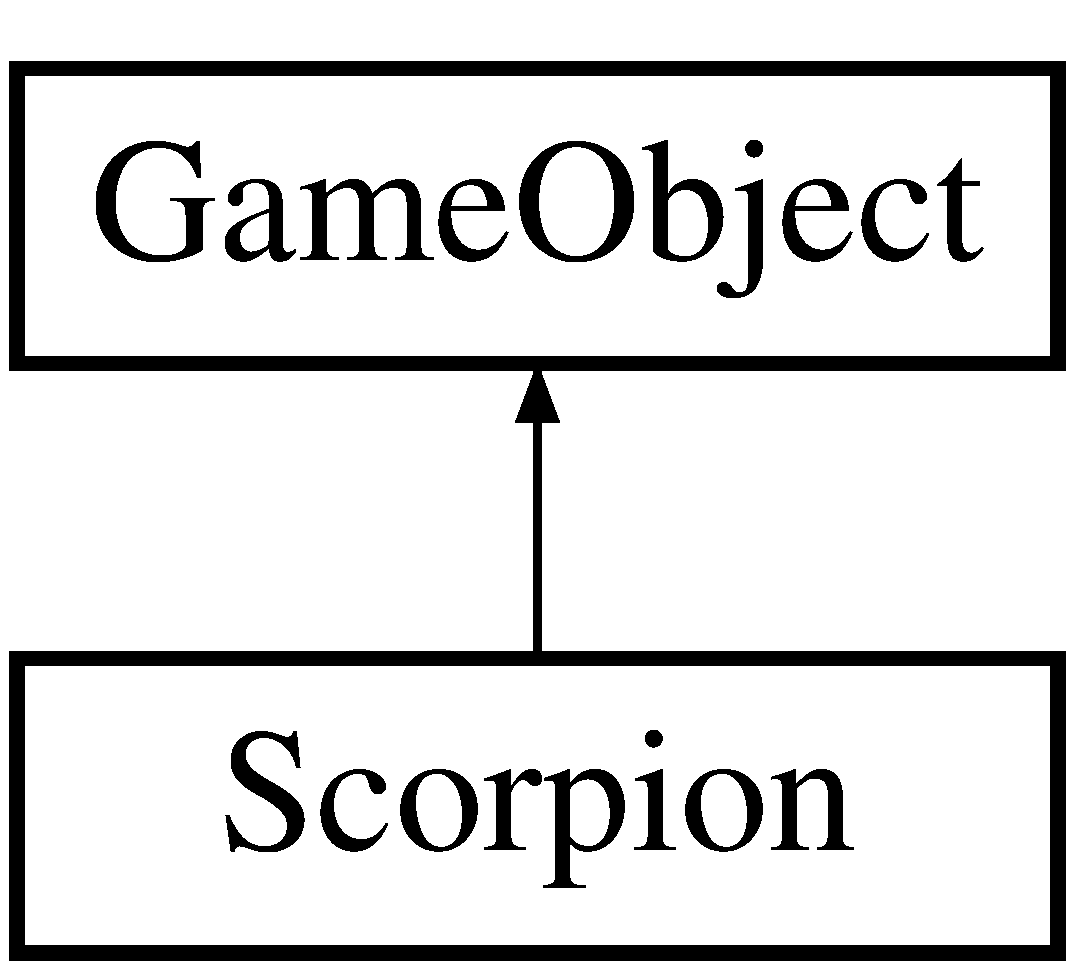
\includegraphics[height=2.000000cm]{class_scorpion}
\end{center}
\end{figure}
\subsection*{Public Member Functions}
\begin{DoxyCompactItemize}
\item 
\mbox{\hyperlink{class_scorpion_a0046bcdb8f478bf54032acba20ba44e5}{Scorpion}} (const \mbox{\hyperlink{classvector2_d}{vector2D}} \&size, const \mbox{\hyperlink{classvector2_d}{vector2D}} \&position, float speed, Object\+ID objectid)
\begin{DoxyCompactList}\small\item\em Constructor of the \mbox{\hyperlink{class_scorpion}{Scorpion}} Class. \end{DoxyCompactList}\item 
\mbox{\Hypertarget{class_scorpion_a4f5a88977dd4dd19dd5c61a8114f43a5}\label{class_scorpion_a4f5a88977dd4dd19dd5c61a8114f43a5}} 
virtual void \mbox{\hyperlink{class_scorpion_a4f5a88977dd4dd19dd5c61a8114f43a5}{collision\+Response}} () override
\begin{DoxyCompactList}\small\item\em Take action if \mbox{\hyperlink{class_scorpion}{Scorpion}} is shot. \end{DoxyCompactList}\item 
\mbox{\Hypertarget{class_scorpion_acf8d302a008882781a701df5854d2c75}\label{class_scorpion_acf8d302a008882781a701df5854d2c75}} 
virtual void \mbox{\hyperlink{class_scorpion_acf8d302a008882781a701df5854d2c75}{Move}} () override
\begin{DoxyCompactList}\small\item\em Move function from parent. \end{DoxyCompactList}\item 
\mbox{\Hypertarget{class_scorpion_a9de22ed90e1a48e06291317fbe558e41}\label{class_scorpion_a9de22ed90e1a48e06291317fbe558e41}} 
virtual void \mbox{\hyperlink{class_scorpion_a9de22ed90e1a48e06291317fbe558e41}{reset}} () override
\begin{DoxyCompactList}\small\item\em Reset \mbox{\hyperlink{class_scorpion}{Scorpion}} to intial conditions. \end{DoxyCompactList}\item 
\mbox{\Hypertarget{class_scorpion_af44080430b68b2f9ea07b3cc9df03453}\label{class_scorpion_af44080430b68b2f9ea07b3cc9df03453}} 
virtual \mbox{\hyperlink{class_scorpion_af44080430b68b2f9ea07b3cc9df03453}{$\sim$\+Scorpion}} ()
\begin{DoxyCompactList}\small\item\em Destroy the \mbox{\hyperlink{class_scorpion}{Scorpion}} Object. \end{DoxyCompactList}\end{DoxyCompactItemize}
\subsection*{Private Member Functions}
\begin{DoxyCompactItemize}
\item 
\mbox{\Hypertarget{class_scorpion_ac455b0a8472ddfec0c8a3e2bef8e87a6}\label{class_scorpion_ac455b0a8472ddfec0c8a3e2bef8e87a6}} 
void \mbox{\hyperlink{class_scorpion_ac455b0a8472ddfec0c8a3e2bef8e87a6}{move\+Left}} ()
\begin{DoxyCompactList}\small\item\em move \mbox{\hyperlink{class_scorpion}{Scorpion}} to the left direction \end{DoxyCompactList}\item 
\mbox{\Hypertarget{class_scorpion_a6220ca4cfc5c17f4a96ab4e35b198bc7}\label{class_scorpion_a6220ca4cfc5c17f4a96ab4e35b198bc7}} 
void \mbox{\hyperlink{class_scorpion_a6220ca4cfc5c17f4a96ab4e35b198bc7}{move\+Right}} ()
\begin{DoxyCompactList}\small\item\em move \mbox{\hyperlink{class_scorpion}{Scorpion}} to the right direction \end{DoxyCompactList}\item 
\mbox{\Hypertarget{class_scorpion_a039d9e95b6e72d6d6767e3ffe0160aa6}\label{class_scorpion_a039d9e95b6e72d6d6767e3ffe0160aa6}} 
void \mbox{\hyperlink{class_scorpion_a039d9e95b6e72d6d6767e3ffe0160aa6}{right\+Reset}} ()
\begin{DoxyCompactList}\small\item\em reset the scorpion to start at the right \end{DoxyCompactList}\item 
\mbox{\Hypertarget{class_scorpion_aaf8a8405cf42b12bfac85c25880e1447}\label{class_scorpion_aaf8a8405cf42b12bfac85c25880e1447}} 
void \mbox{\hyperlink{class_scorpion_aaf8a8405cf42b12bfac85c25880e1447}{left\+Reset}} ()
\begin{DoxyCompactList}\small\item\em reset the scorpion to start at the left \end{DoxyCompactList}\end{DoxyCompactItemize}
\subsection*{Private Attributes}
\begin{DoxyCompactItemize}
\item 
\mbox{\Hypertarget{class_scorpion_a9cb4ba3041279cfc5463f53544606e88}\label{class_scorpion_a9cb4ba3041279cfc5463f53544606e88}} 
bool {\bfseries forward\+\_\+} = true
\end{DoxyCompactItemize}


\subsection{Detailed Description}
\begin{DoxyDate}{Date}
08/10/2018 
\end{DoxyDate}


\subsection{Constructor \& Destructor Documentation}
\mbox{\Hypertarget{class_scorpion_a0046bcdb8f478bf54032acba20ba44e5}\label{class_scorpion_a0046bcdb8f478bf54032acba20ba44e5}} 
\index{Scorpion@{Scorpion}!Scorpion@{Scorpion}}
\index{Scorpion@{Scorpion}!Scorpion@{Scorpion}}
\subsubsection{\texorpdfstring{Scorpion()}{Scorpion()}}
{\footnotesize\ttfamily Scorpion\+::\+Scorpion (\begin{DoxyParamCaption}\item[{const \mbox{\hyperlink{classvector2_d}{vector2D}} \&}]{size,  }\item[{const \mbox{\hyperlink{classvector2_d}{vector2D}} \&}]{position,  }\item[{float}]{speed,  }\item[{Object\+ID}]{objectid }\end{DoxyParamCaption})\hspace{0.3cm}{\ttfamily [inline]}}



Constructor of the \mbox{\hyperlink{class_scorpion}{Scorpion}} Class. 


\begin{DoxyParams}{Parameters}
{\em size} & of the \mbox{\hyperlink{class_scorpion}{Scorpion}} \\
\hline
{\em position} & of the \mbox{\hyperlink{class_scorpion}{Scorpion}} \\
\hline
{\em speed} & of the \mbox{\hyperlink{class_scorpion}{Scorpion}} \\
\hline
{\em objectid} & ID of the \mbox{\hyperlink{class_scorpion}{Scorpion}} \\
\hline
\end{DoxyParams}


The documentation for this class was generated from the following files\+:\begin{DoxyCompactItemize}
\item 
C\+:/\+Users/bvrad/\+Dropbox/\+Boikanyo/elen3009/\+P\+R\+O\+J\+E\+C\+T/2018-\/project-\/1386807-\/\+Radiokana-\/1427726-\/\+Sepuru/game-\/source-\/code/\mbox{\hyperlink{_scorpion_8h}{Scorpion.\+h}}\item 
C\+:/\+Users/bvrad/\+Dropbox/\+Boikanyo/elen3009/\+P\+R\+O\+J\+E\+C\+T/2018-\/project-\/1386807-\/\+Radiokana-\/1427726-\/\+Sepuru/game-\/source-\/code/Scorpion.\+cpp\end{DoxyCompactItemize}

\hypertarget{class_spaceship}{}\section{Spaceship Class Reference}
\label{class_spaceship}\index{Spaceship@{Spaceship}}


{\ttfamily \#include $<$Spaceship.\+h$>$}

Inheritance diagram for Spaceship\+:\begin{figure}[H]
\begin{center}
\leavevmode
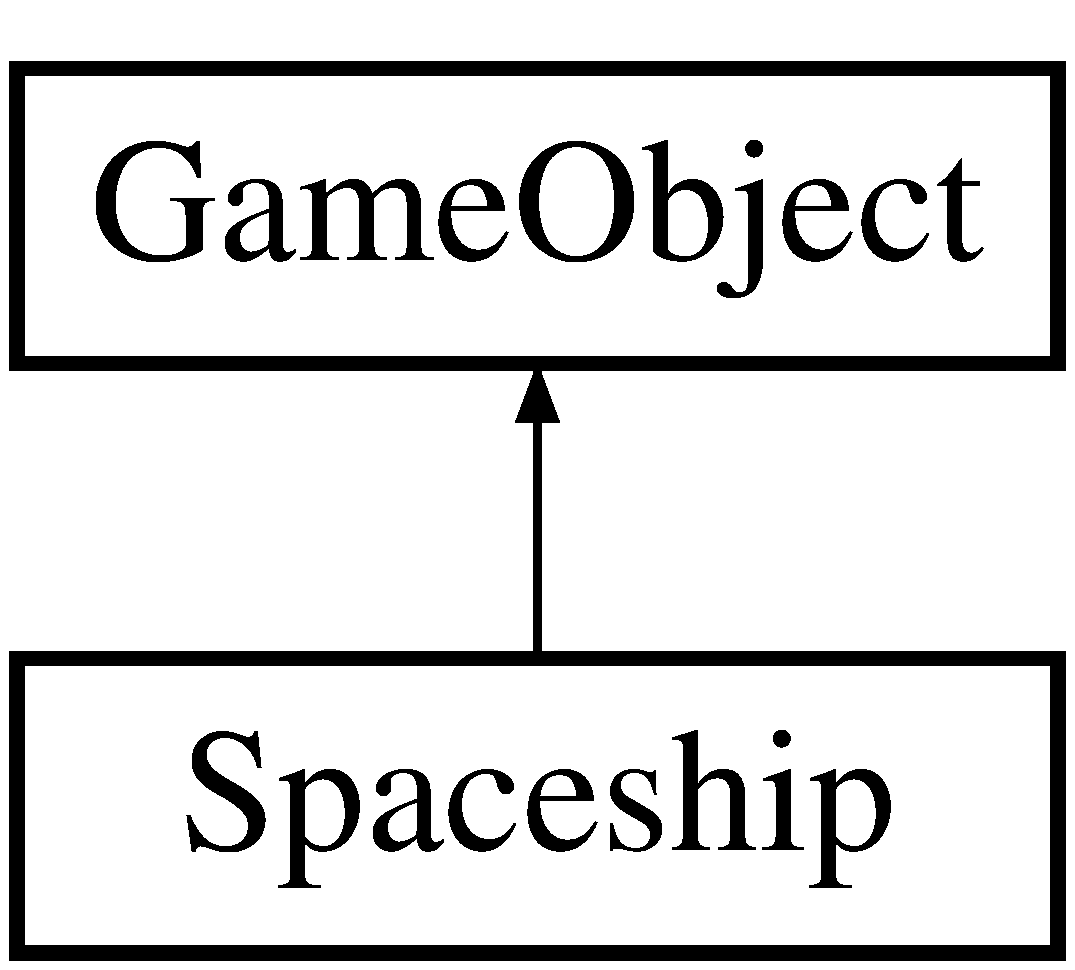
\includegraphics[height=2.000000cm]{class_spaceship}
\end{center}
\end{figure}
\subsection*{Public Member Functions}
\begin{DoxyCompactItemize}
\item 
\mbox{\hyperlink{class_spaceship_a3fe713cbac3c0c20c298ab1d1aa13a71}{Spaceship}} (const \mbox{\hyperlink{classvector2_d}{vector2D}} \&size, const \mbox{\hyperlink{classvector2_d}{vector2D}} \&position, float speed, Object\+ID objectid)
\begin{DoxyCompactList}\small\item\em Constructor of the \mbox{\hyperlink{class_spaceship}{Spaceship}} Class. \end{DoxyCompactList}\item 
\mbox{\Hypertarget{class_spaceship_ad82228c11cdc42ce2279756de72e134b}\label{class_spaceship_ad82228c11cdc42ce2279756de72e134b}} 
virtual void \mbox{\hyperlink{class_spaceship_ad82228c11cdc42ce2279756de72e134b}{Move}} () override
\begin{DoxyCompactList}\small\item\em Game Object moves is not used for \mbox{\hyperlink{class_spaceship}{Spaceship}}. \end{DoxyCompactList}\item 
std\+::tuple$<$ std\+::shared\+\_\+ptr$<$ \mbox{\hyperlink{class_lazer_shot}{Lazer\+Shot}} $>$, int $>$ \mbox{\hyperlink{class_spaceship_aa8f630847912cacefb0f3494ae8d0480}{fired\+Lazer\+Shot}} (int i) const
\begin{DoxyCompactList}\small\item\em Return fired lazer shot. \end{DoxyCompactList}\item 
\mbox{\Hypertarget{class_spaceship_ac14518da6eb7c15d5e34d65a9929dcdd}\label{class_spaceship_ac14518da6eb7c15d5e34d65a9929dcdd}} 
void \mbox{\hyperlink{class_spaceship_ac14518da6eb7c15d5e34d65a9929dcdd}{load}} ()
\begin{DoxyCompactList}\small\item\em Load the \mbox{\hyperlink{class_lazer_shot}{Lazer\+Shot}} gun of the \mbox{\hyperlink{class_spaceship}{Spaceship}}. \end{DoxyCompactList}\item 
\mbox{\Hypertarget{class_spaceship_af29256d4fa2c28f773dd26ce74c22d15}\label{class_spaceship_af29256d4fa2c28f773dd26ce74c22d15}} 
void \mbox{\hyperlink{class_spaceship_af29256d4fa2c28f773dd26ce74c22d15}{shoot}} ()
\begin{DoxyCompactList}\small\item\em Fire at the at the target. \end{DoxyCompactList}\item 
\mbox{\Hypertarget{class_spaceship_a47911214849b05082ee0876a3b8bac7a}\label{class_spaceship_a47911214849b05082ee0876a3b8bac7a}} 
virtual void \mbox{\hyperlink{class_spaceship_a47911214849b05082ee0876a3b8bac7a}{collision\+Response}} () override
\begin{DoxyCompactList}\small\item\em Explode the \mbox{\hyperlink{class_spaceship}{Spaceship}}. \end{DoxyCompactList}\item 
\mbox{\Hypertarget{class_spaceship_a8f1eabe7d82fe9d517266ce5f111d421}\label{class_spaceship_a8f1eabe7d82fe9d517266ce5f111d421}} 
void \mbox{\hyperlink{class_spaceship_a8f1eabe7d82fe9d517266ce5f111d421}{lost\+Life}} ()
\begin{DoxyCompactList}\small\item\em Decreement the number of lives. \end{DoxyCompactList}\item 
int \mbox{\hyperlink{class_spaceship_a5b7b351757965153332a4e66ef8e0b61}{Lives}} ()
\begin{DoxyCompactList}\small\item\em Get number of lives. \end{DoxyCompactList}\item 
void \mbox{\hyperlink{class_spaceship_a02a31fd44b5b9f60743d1e04f10fa113}{Lives}} (int lives)
\begin{DoxyCompactList}\small\item\em Set Number of lives. \end{DoxyCompactList}\item 
\mbox{\Hypertarget{class_spaceship_a78bb6c136c35d3f43f3937732ccb1de2}\label{class_spaceship_a78bb6c136c35d3f43f3937732ccb1de2}} 
virtual void \mbox{\hyperlink{class_spaceship_a78bb6c136c35d3f43f3937732ccb1de2}{reset}} () override
\begin{DoxyCompactList}\small\item\em Reset \mbox{\hyperlink{class_spaceship}{Spaceship}} to inital conditions. \end{DoxyCompactList}\item 
\mbox{\Hypertarget{class_spaceship_aaf51352795ea2382e2aaea4b9a058804}\label{class_spaceship_aaf51352795ea2382e2aaea4b9a058804}} 
virtual \mbox{\hyperlink{class_spaceship_aaf51352795ea2382e2aaea4b9a058804}{$\sim$\+Spaceship}} ()
\begin{DoxyCompactList}\small\item\em Destructor. \end{DoxyCompactList}\end{DoxyCompactItemize}
\subsection*{Private Attributes}
\begin{DoxyCompactItemize}
\item 
\mbox{\Hypertarget{class_spaceship_ac8fad23e2d21d360fbbcd3f13a650a6e}\label{class_spaceship_ac8fad23e2d21d360fbbcd3f13a650a6e}} 
int {\bfseries lives\+\_\+} = 3
\item 
\mbox{\Hypertarget{class_spaceship_ae2d6c0ce59cd20a0445c02686a3e8b16}\label{class_spaceship_ae2d6c0ce59cd20a0445c02686a3e8b16}} 
int {\bfseries no\+Of\+Lazer\+Shots\+\_\+} = 0
\item 
\mbox{\Hypertarget{class_spaceship_a1ab5797ea77593a72c11e4825e000856}\label{class_spaceship_a1ab5797ea77593a72c11e4825e000856}} 
std\+::vector$<$ std\+::shared\+\_\+ptr$<$ \mbox{\hyperlink{class_lazer_shot}{Lazer\+Shot}} $>$ $>$ {\bfseries lazer\+Shots\+Gun\+\_\+}
\end{DoxyCompactItemize}


\subsection{Detailed Description}
\begin{DoxyDate}{Date}
08/10/2018 
\end{DoxyDate}


\subsection{Constructor \& Destructor Documentation}
\mbox{\Hypertarget{class_spaceship_a3fe713cbac3c0c20c298ab1d1aa13a71}\label{class_spaceship_a3fe713cbac3c0c20c298ab1d1aa13a71}} 
\index{Spaceship@{Spaceship}!Spaceship@{Spaceship}}
\index{Spaceship@{Spaceship}!Spaceship@{Spaceship}}
\subsubsection{\texorpdfstring{Spaceship()}{Spaceship()}}
{\footnotesize\ttfamily Spaceship\+::\+Spaceship (\begin{DoxyParamCaption}\item[{const \mbox{\hyperlink{classvector2_d}{vector2D}} \&}]{size,  }\item[{const \mbox{\hyperlink{classvector2_d}{vector2D}} \&}]{position,  }\item[{float}]{speed,  }\item[{Object\+ID}]{objectid }\end{DoxyParamCaption})\hspace{0.3cm}{\ttfamily [inline]}}



Constructor of the \mbox{\hyperlink{class_spaceship}{Spaceship}} Class. 


\begin{DoxyParams}{Parameters}
{\em size} & of the \mbox{\hyperlink{class_spaceship}{Spaceship}} \\
\hline
{\em position} & of the \mbox{\hyperlink{class_spaceship}{Spaceship}} \\
\hline
{\em speed} & of the \mbox{\hyperlink{class_spaceship}{Spaceship}} \\
\hline
{\em objectid} & ID of the \mbox{\hyperlink{class_spaceship}{Spaceship}} \\
\hline
\end{DoxyParams}


\subsection{Member Function Documentation}
\mbox{\Hypertarget{class_spaceship_aa8f630847912cacefb0f3494ae8d0480}\label{class_spaceship_aa8f630847912cacefb0f3494ae8d0480}} 
\index{Spaceship@{Spaceship}!fired\+Lazer\+Shot@{fired\+Lazer\+Shot}}
\index{fired\+Lazer\+Shot@{fired\+Lazer\+Shot}!Spaceship@{Spaceship}}
\subsubsection{\texorpdfstring{fired\+Lazer\+Shot()}{firedLazerShot()}}
{\footnotesize\ttfamily std\+::tuple$<$std\+::shared\+\_\+ptr$<$\mbox{\hyperlink{class_lazer_shot}{Lazer\+Shot}}$>$,int$>$ Spaceship\+::fired\+Lazer\+Shot (\begin{DoxyParamCaption}\item[{int}]{i }\end{DoxyParamCaption}) const\hspace{0.3cm}{\ttfamily [inline]}}



Return fired lazer shot. 


\begin{DoxyParams}{Parameters}
{\em i} & iterator to Lazer\+Shots Container \\
\hline
\end{DoxyParams}
\begin{DoxyReturn}{Returns}
\mbox{\hyperlink{class_lazer_shot}{Lazer\+Shot}} 
\end{DoxyReturn}
\mbox{\Hypertarget{class_spaceship_a5b7b351757965153332a4e66ef8e0b61}\label{class_spaceship_a5b7b351757965153332a4e66ef8e0b61}} 
\index{Spaceship@{Spaceship}!Lives@{Lives}}
\index{Lives@{Lives}!Spaceship@{Spaceship}}
\subsubsection{\texorpdfstring{Lives()}{Lives()}\hspace{0.1cm}{\footnotesize\ttfamily [1/2]}}
{\footnotesize\ttfamily int Spaceship\+::\+Lives (\begin{DoxyParamCaption}{ }\end{DoxyParamCaption})\hspace{0.3cm}{\ttfamily [inline]}}



Get number of lives. 

\begin{DoxyReturn}{Returns}
numver of lives 
\end{DoxyReturn}
\mbox{\Hypertarget{class_spaceship_a02a31fd44b5b9f60743d1e04f10fa113}\label{class_spaceship_a02a31fd44b5b9f60743d1e04f10fa113}} 
\index{Spaceship@{Spaceship}!Lives@{Lives}}
\index{Lives@{Lives}!Spaceship@{Spaceship}}
\subsubsection{\texorpdfstring{Lives()}{Lives()}\hspace{0.1cm}{\footnotesize\ttfamily [2/2]}}
{\footnotesize\ttfamily void Spaceship\+::\+Lives (\begin{DoxyParamCaption}\item[{int}]{lives }\end{DoxyParamCaption})\hspace{0.3cm}{\ttfamily [inline]}}



Set Number of lives. 


\begin{DoxyParams}{Parameters}
{\em lives} & is the number of lives to be set \\
\hline
\end{DoxyParams}


The documentation for this class was generated from the following files\+:\begin{DoxyCompactItemize}
\item 
C\+:/\+Users/bvrad/\+Dropbox/\+Boikanyo/elen3009/\+P\+R\+O\+J\+E\+C\+T/2018-\/project-\/1386807-\/\+Radiokana-\/1427726-\/\+Sepuru/game-\/source-\/code/\mbox{\hyperlink{_spaceship_8h}{Spaceship.\+h}}\item 
C\+:/\+Users/bvrad/\+Dropbox/\+Boikanyo/elen3009/\+P\+R\+O\+J\+E\+C\+T/2018-\/project-\/1386807-\/\+Radiokana-\/1427726-\/\+Sepuru/game-\/source-\/code/Spaceship.\+cpp\end{DoxyCompactItemize}

\hypertarget{class_spider}{}\section{Spider Class Reference}
\label{class_spider}\index{Spider@{Spider}}


{\ttfamily \#include $<$Spider.\+h$>$}

Inheritance diagram for Spider\+:\begin{figure}[H]
\begin{center}
\leavevmode
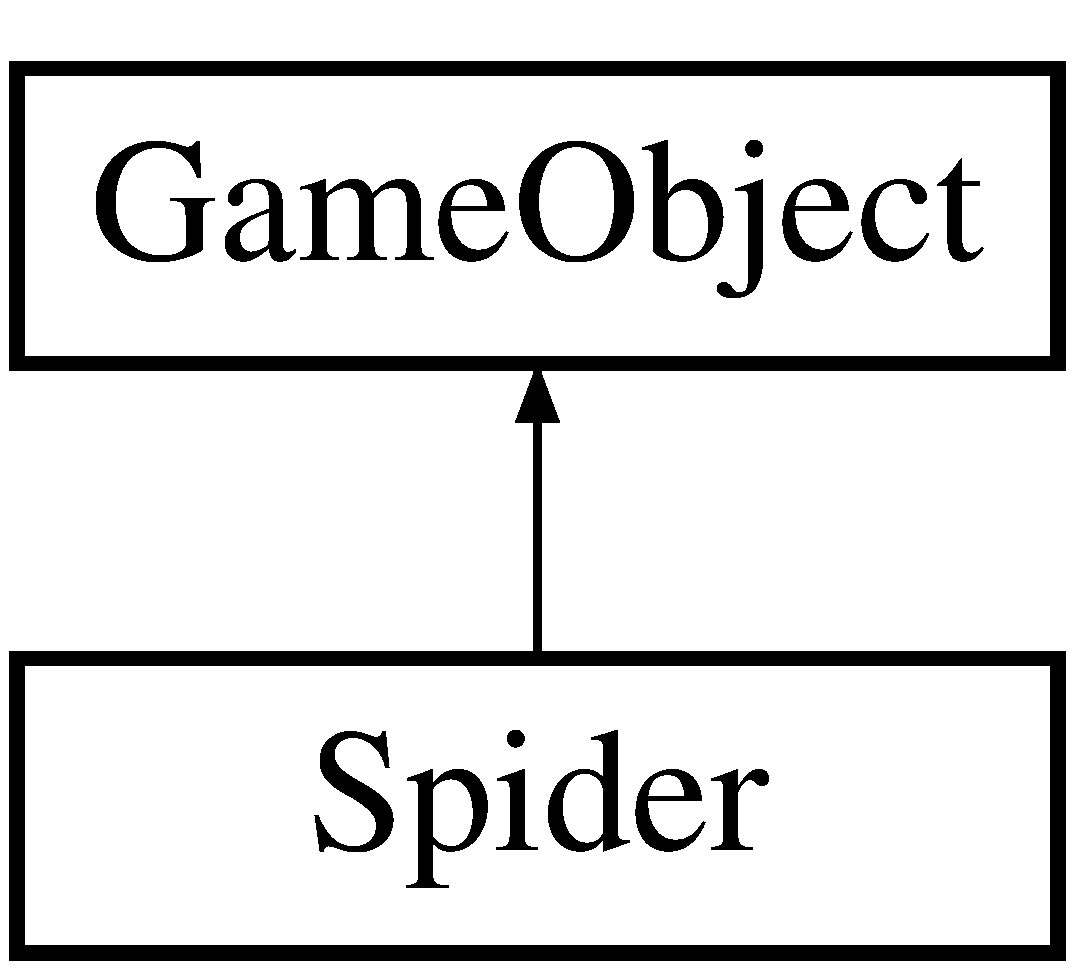
\includegraphics[height=2.000000cm]{class_spider}
\end{center}
\end{figure}
\subsection*{Public Member Functions}
\begin{DoxyCompactItemize}
\item 
\mbox{\hyperlink{class_spider_afa46831c19ecd0e22b1b186cf3ff38d8}{Spider}} (const \mbox{\hyperlink{classvector2_d}{vector2D}} \&size, const \mbox{\hyperlink{classvector2_d}{vector2D}} \&position, float speed, Object\+ID objectid)
\begin{DoxyCompactList}\small\item\em Constructor of the \mbox{\hyperlink{class_spider}{Spider}} Class. \end{DoxyCompactList}\item 
\mbox{\Hypertarget{class_spider_a7a5c1f3cfa2c11f1167cea5a4fff32d5}\label{class_spider_a7a5c1f3cfa2c11f1167cea5a4fff32d5}} 
virtual void \mbox{\hyperlink{class_spider_a7a5c1f3cfa2c11f1167cea5a4fff32d5}{Move}} () override
\begin{DoxyCompactList}\small\item\em Move \mbox{\hyperlink{class_spider}{Spider}} Across Screen. \end{DoxyCompactList}\item 
\mbox{\Hypertarget{class_spider_a99d8b17abd435ac612ec05cfa49839ec}\label{class_spider_a99d8b17abd435ac612ec05cfa49839ec}} 
virtual void \mbox{\hyperlink{class_spider_a99d8b17abd435ac612ec05cfa49839ec}{reset}} () override
\begin{DoxyCompactList}\small\item\em Reset \mbox{\hyperlink{class_spider}{Spider}} to initial conditions. \end{DoxyCompactList}\item 
\mbox{\Hypertarget{class_spider_a5548b1fc8a2dfc3be40cf06ed13e698f}\label{class_spider_a5548b1fc8a2dfc3be40cf06ed13e698f}} 
virtual void \mbox{\hyperlink{class_spider_a5548b1fc8a2dfc3be40cf06ed13e698f}{collision\+Response}} () override
\begin{DoxyCompactList}\small\item\em Explode the spider. \end{DoxyCompactList}\item 
\mbox{\Hypertarget{class_spider_a1f6a4d46d39696b253a924effb156971}\label{class_spider_a1f6a4d46d39696b253a924effb156971}} 
virtual \mbox{\hyperlink{class_spider_a1f6a4d46d39696b253a924effb156971}{$\sim$\+Spider}} ()
\begin{DoxyCompactList}\small\item\em Destroy the Object. \end{DoxyCompactList}\end{DoxyCompactItemize}
\subsection*{Private Member Functions}
\begin{DoxyCompactItemize}
\item 
\mbox{\Hypertarget{class_spider_ace407f694d63ed88367963310747c739}\label{class_spider_ace407f694d63ed88367963310747c739}} 
void \mbox{\hyperlink{class_spider_ace407f694d63ed88367963310747c739}{move\+Down}} ()
\begin{DoxyCompactList}\small\item\em For down movement. \end{DoxyCompactList}\item 
\mbox{\Hypertarget{class_spider_a456d9495aca3a636e584b3d8678596fd}\label{class_spider_a456d9495aca3a636e584b3d8678596fd}} 
void \mbox{\hyperlink{class_spider_a456d9495aca3a636e584b3d8678596fd}{move\+Up}} ()
\begin{DoxyCompactList}\small\item\em For up movement. \end{DoxyCompactList}\item 
\mbox{\Hypertarget{class_spider_a7ef566f45e66889f34b3e9d058ac58d0}\label{class_spider_a7ef566f45e66889f34b3e9d058ac58d0}} 
void \mbox{\hyperlink{class_spider_a7ef566f45e66889f34b3e9d058ac58d0}{move\+Zig}} ()
\begin{DoxyCompactList}\small\item\em Up movement left or right. \end{DoxyCompactList}\item 
\mbox{\Hypertarget{class_spider_a64bb1061c1e7bf1a3598e817bffe3538}\label{class_spider_a64bb1061c1e7bf1a3598e817bffe3538}} 
void \mbox{\hyperlink{class_spider_a64bb1061c1e7bf1a3598e817bffe3538}{move\+Zag}} ()
\begin{DoxyCompactList}\small\item\em Down movement left or right. \end{DoxyCompactList}\end{DoxyCompactItemize}
\subsection*{Private Attributes}
\begin{DoxyCompactItemize}
\item 
\mbox{\Hypertarget{class_spider_adc12c0ff82343b7123401aa7fd53fca8}\label{class_spider_adc12c0ff82343b7123401aa7fd53fca8}} 
bool {\bfseries zigzag\+\_\+} = true
\item 
\mbox{\Hypertarget{class_spider_a2bcc5037a10a7995cb10f7be6299780b}\label{class_spider_a2bcc5037a10a7995cb10f7be6299780b}} 
bool {\bfseries up\+\_\+} = false
\end{DoxyCompactItemize}


\subsection{Detailed Description}
\begin{DoxyDate}{Date}
08/10/2018 
\end{DoxyDate}


\subsection{Constructor \& Destructor Documentation}
\mbox{\Hypertarget{class_spider_afa46831c19ecd0e22b1b186cf3ff38d8}\label{class_spider_afa46831c19ecd0e22b1b186cf3ff38d8}} 
\index{Spider@{Spider}!Spider@{Spider}}
\index{Spider@{Spider}!Spider@{Spider}}
\subsubsection{\texorpdfstring{Spider()}{Spider()}}
{\footnotesize\ttfamily Spider\+::\+Spider (\begin{DoxyParamCaption}\item[{const \mbox{\hyperlink{classvector2_d}{vector2D}} \&}]{size,  }\item[{const \mbox{\hyperlink{classvector2_d}{vector2D}} \&}]{position,  }\item[{float}]{speed,  }\item[{Object\+ID}]{objectid }\end{DoxyParamCaption})\hspace{0.3cm}{\ttfamily [inline]}}



Constructor of the \mbox{\hyperlink{class_spider}{Spider}} Class. 


\begin{DoxyParams}{Parameters}
{\em size} & of the \mbox{\hyperlink{class_spider}{Spider}} \\
\hline
{\em position} & of the \mbox{\hyperlink{class_spider}{Spider}} \\
\hline
{\em speed} & of the \mbox{\hyperlink{class_spider}{Spider}} \\
\hline
{\em objectid} & ID of the \mbox{\hyperlink{class_spider}{Spider}} \\
\hline
\end{DoxyParams}


The documentation for this class was generated from the following files\+:\begin{DoxyCompactItemize}
\item 
C\+:/\+Users/bvrad/\+Dropbox/\+Boikanyo/elen3009/\+P\+R\+O\+J\+E\+C\+T/2018-\/project-\/1386807-\/\+Radiokana-\/1427726-\/\+Sepuru/game-\/source-\/code/\mbox{\hyperlink{_spider_8h}{Spider.\+h}}\item 
C\+:/\+Users/bvrad/\+Dropbox/\+Boikanyo/elen3009/\+P\+R\+O\+J\+E\+C\+T/2018-\/project-\/1386807-\/\+Radiokana-\/1427726-\/\+Sepuru/game-\/source-\/code/Spider.\+cpp\end{DoxyCompactItemize}

\hypertarget{class_splash_screen}{}\section{Splash\+Screen Class Reference}
\label{class_splash_screen}\index{Splash\+Screen@{Splash\+Screen}}


{\ttfamily \#include $<$Splash\+Screen.\+h$>$}

\subsection*{Public Member Functions}
\begin{DoxyCompactItemize}
\item 
\mbox{\Hypertarget{class_splash_screen_a1e61f315445dd725cdbeac840e9bba17}\label{class_splash_screen_a1e61f315445dd725cdbeac840e9bba17}} 
{\bfseries Splash\+Screen} (shared\+\_\+ptr$<$ \mbox{\hyperlink{class_display}{Display}} $>$ display\+\_\+ptr)
\item 
\mbox{\Hypertarget{class_splash_screen_a3bf88eb0bf0940a7ffd265a9963db192}\label{class_splash_screen_a3bf88eb0bf0940a7ffd265a9963db192}} 
void \mbox{\hyperlink{class_splash_screen_a3bf88eb0bf0940a7ffd265a9963db192}{Opening\+Screen}} ()
\begin{DoxyCompactList}\small\item\em Draws the opening screen. \end{DoxyCompactList}\item 
\mbox{\Hypertarget{class_splash_screen_a972f1af2a9adf8fd18c934aa703f4c80}\label{class_splash_screen_a972f1af2a9adf8fd18c934aa703f4c80}} 
void \mbox{\hyperlink{class_splash_screen_a972f1af2a9adf8fd18c934aa703f4c80}{Help\+Screen}} ()
\begin{DoxyCompactList}\small\item\em Draws the helpscreen. \end{DoxyCompactList}\item 
void \mbox{\hyperlink{class_splash_screen_a0fec044f81b02f9ba6c94ca9ed01d100}{You\+Loose}} (int score)
\begin{DoxyCompactList}\small\item\em Draws the game over screen. \end{DoxyCompactList}\item 
void \mbox{\hyperlink{class_splash_screen_a239fe0cad561285bd029a8042c2a8039}{Game\+Screen}} (shared\+\_\+ptr$<$ \mbox{\hyperlink{class_score}{Score}} $>$ score\+\_\+ptr, int lives)
\begin{DoxyCompactList}\small\item\em Draws the Background of the gamescreen. \end{DoxyCompactList}\item 
\mbox{\Hypertarget{class_splash_screen_a8a91ffe9d78177da94607a9876621850}\label{class_splash_screen_a8a91ffe9d78177da94607a9876621850}} 
void \mbox{\hyperlink{class_splash_screen_a8a91ffe9d78177da94607a9876621850}{Pause}} ()
\begin{DoxyCompactList}\small\item\em Pause Message. \end{DoxyCompactList}\item 
\mbox{\Hypertarget{class_splash_screen_a98a24e3b73ea0c4500cb6a50316509ba}\label{class_splash_screen_a98a24e3b73ea0c4500cb6a50316509ba}} 
void \mbox{\hyperlink{class_splash_screen_a98a24e3b73ea0c4500cb6a50316509ba}{get\+Ready}} ()
\begin{DoxyCompactList}\small\item\em In between Message. \end{DoxyCompactList}\item 
Screen\+Object\+ID \mbox{\hyperlink{class_splash_screen_a9ee25ec3f5cf41323a5fc4f99b2b1016}{Detect\+Button}} ()
\begin{DoxyCompactList}\small\item\em Detects which button in the screen is being pressed. \end{DoxyCompactList}\end{DoxyCompactItemize}
\subsection*{Private Member Functions}
\begin{DoxyCompactItemize}
\item 
std\+::tuple$<$ float, float, float, float $>$ \mbox{\hyperlink{class_splash_screen_aee2130b85a0f8850816f155cf8c4800b}{Button\+Dimension}} (sf\+::\+Rectangle\+Shape button)
\begin{DoxyCompactList}\small\item\em Gets dimensions of the buttons. \end{DoxyCompactList}\item 
sf\+::\+Rectangle\+Shape \mbox{\hyperlink{class_splash_screen_af34b1a6b28c5fe8f4124ff7d94be6c55}{Draw\+Screen\+Object}} (const \mbox{\hyperlink{classvector2_d}{vector2D}} \&size, const \mbox{\hyperlink{classvector2_d}{vector2D}} \&position, Screen\+Object\+ID ID)
\begin{DoxyCompactList}\small\item\em Makes buttons. \end{DoxyCompactList}\item 
void \mbox{\hyperlink{class_splash_screen_ae617c148840201b21946e718414748f4}{High\+Scores}} (int score)
\begin{DoxyCompactList}\small\item\em Draws high scores. \end{DoxyCompactList}\end{DoxyCompactItemize}
\subsection*{Private Attributes}
\begin{DoxyCompactItemize}
\item 
\mbox{\Hypertarget{class_splash_screen_a6e5534a8525379af86dff12d7a973a35}\label{class_splash_screen_a6e5534a8525379af86dff12d7a973a35}} 
shared\+\_\+ptr$<$ sf\+::\+Render\+Window $>$ {\bfseries window\+\_\+}
\item 
\mbox{\Hypertarget{class_splash_screen_ab07847d1ec31f99737ad2a3131c4d985}\label{class_splash_screen_ab07847d1ec31f99737ad2a3131c4d985}} 
std\+::vector$<$ sf\+::\+Texture $>$ {\bfseries screen\+Object\+Textures\+\_\+}
\item 
\mbox{\Hypertarget{class_splash_screen_aafcefbb104c701194a6ae390d3c1015f}\label{class_splash_screen_aafcefbb104c701194a6ae390d3c1015f}} 
float {\bfseries a}
\item 
\mbox{\Hypertarget{class_splash_screen_a9e97934c6104c7df599089ca4fd64f11}\label{class_splash_screen_a9e97934c6104c7df599089ca4fd64f11}} 
float {\bfseries b}
\item 
\mbox{\Hypertarget{class_splash_screen_a74b76a6b24b334f0244440305193e457}\label{class_splash_screen_a74b76a6b24b334f0244440305193e457}} 
float {\bfseries c}
\item 
\mbox{\Hypertarget{class_splash_screen_a474a4444e35bda0797985eef2f642c3c}\label{class_splash_screen_a474a4444e35bda0797985eef2f642c3c}} 
float {\bfseries d}
\item 
\mbox{\Hypertarget{class_splash_screen_a7fa565ee936d4a022b68b4b92fdfa66c}\label{class_splash_screen_a7fa565ee936d4a022b68b4b92fdfa66c}} 
float {\bfseries e}
\item 
\mbox{\Hypertarget{class_splash_screen_a114b8336b153cfbd25053ee6857432f7}\label{class_splash_screen_a114b8336b153cfbd25053ee6857432f7}} 
float {\bfseries f}
\item 
\mbox{\Hypertarget{class_splash_screen_ad2532945a72a48c68f6f6f8da8d27707}\label{class_splash_screen_ad2532945a72a48c68f6f6f8da8d27707}} 
float {\bfseries g}
\item 
\mbox{\Hypertarget{class_splash_screen_a59151d152682fd4f8e7f69da9cfd9e43}\label{class_splash_screen_a59151d152682fd4f8e7f69da9cfd9e43}} 
float {\bfseries h}
\item 
\mbox{\Hypertarget{class_splash_screen_aff4c9ec4c870cd11f9510da0593b895f}\label{class_splash_screen_aff4c9ec4c870cd11f9510da0593b895f}} 
float {\bfseries q}
\item 
\mbox{\Hypertarget{class_splash_screen_a7c4400cf529a50573bd114fb00073e92}\label{class_splash_screen_a7c4400cf529a50573bd114fb00073e92}} 
float {\bfseries r}
\item 
\mbox{\Hypertarget{class_splash_screen_ad7b085e2cbee7c5c8df8f339efc6fe6e}\label{class_splash_screen_ad7b085e2cbee7c5c8df8f339efc6fe6e}} 
float {\bfseries w}
\item 
\mbox{\Hypertarget{class_splash_screen_a19cd9ea9c41709c7c448f6bd805301eb}\label{class_splash_screen_a19cd9ea9c41709c7c448f6bd805301eb}} 
float {\bfseries t}
\item 
\mbox{\Hypertarget{class_splash_screen_a96495c24bbd96b03df2ce250ac85c27d}\label{class_splash_screen_a96495c24bbd96b03df2ce250ac85c27d}} 
sf\+::\+Font {\bfseries game\+Font}
\item 
\mbox{\Hypertarget{class_splash_screen_afdf82e128b52d4d84ea5a2918aab60e8}\label{class_splash_screen_afdf82e128b52d4d84ea5a2918aab60e8}} 
sf\+::\+Text {\bfseries game\+Text}
\item 
\mbox{\Hypertarget{class_splash_screen_a9bd638ad81224ec3881bc959589d03fb}\label{class_splash_screen_a9bd638ad81224ec3881bc959589d03fb}} 
bool {\bfseries blink\+\_\+} = true
\item 
\mbox{\Hypertarget{class_splash_screen_a4e0c6dd83de43428c0eb57e03a74cdb9}\label{class_splash_screen_a4e0c6dd83de43428c0eb57e03a74cdb9}} 
\mbox{\hyperlink{class_game_files}{Game\+Files}} {\bfseries gamefile\+\_\+}
\end{DoxyCompactItemize}


\subsection{Detailed Description}
\begin{DoxyAuthor}{Author}
bvrad 
\end{DoxyAuthor}
\begin{DoxyDate}{Date}
08/10/2018 
\end{DoxyDate}


\subsection{Member Function Documentation}
\mbox{\Hypertarget{class_splash_screen_aee2130b85a0f8850816f155cf8c4800b}\label{class_splash_screen_aee2130b85a0f8850816f155cf8c4800b}} 
\index{Splash\+Screen@{Splash\+Screen}!Button\+Dimension@{Button\+Dimension}}
\index{Button\+Dimension@{Button\+Dimension}!Splash\+Screen@{Splash\+Screen}}
\subsubsection{\texorpdfstring{Button\+Dimension()}{ButtonDimension()}}
{\footnotesize\ttfamily std\+::tuple$<$ float, float, float, float $>$ Splash\+Screen\+::\+Button\+Dimension (\begin{DoxyParamCaption}\item[{sf\+::\+Rectangle\+Shape}]{button }\end{DoxyParamCaption})\hspace{0.3cm}{\ttfamily [private]}}



Gets dimensions of the buttons. 


\begin{DoxyParams}{Parameters}
{\em button} & to be drawn \\
\hline
\end{DoxyParams}
\begin{DoxyReturn}{Returns}
button dimensions 
\end{DoxyReturn}
\mbox{\Hypertarget{class_splash_screen_a9ee25ec3f5cf41323a5fc4f99b2b1016}\label{class_splash_screen_a9ee25ec3f5cf41323a5fc4f99b2b1016}} 
\index{Splash\+Screen@{Splash\+Screen}!Detect\+Button@{Detect\+Button}}
\index{Detect\+Button@{Detect\+Button}!Splash\+Screen@{Splash\+Screen}}
\subsubsection{\texorpdfstring{Detect\+Button()}{DetectButton()}}
{\footnotesize\ttfamily Screen\+Object\+ID Splash\+Screen\+::\+Detect\+Button (\begin{DoxyParamCaption}{ }\end{DoxyParamCaption})}



Detects which button in the screen is being pressed. 

\begin{DoxyReturn}{Returns}
ID of Button 
\end{DoxyReturn}
\mbox{\Hypertarget{class_splash_screen_af34b1a6b28c5fe8f4124ff7d94be6c55}\label{class_splash_screen_af34b1a6b28c5fe8f4124ff7d94be6c55}} 
\index{Splash\+Screen@{Splash\+Screen}!Draw\+Screen\+Object@{Draw\+Screen\+Object}}
\index{Draw\+Screen\+Object@{Draw\+Screen\+Object}!Splash\+Screen@{Splash\+Screen}}
\subsubsection{\texorpdfstring{Draw\+Screen\+Object()}{DrawScreenObject()}}
{\footnotesize\ttfamily sf\+::\+Rectangle\+Shape Splash\+Screen\+::\+Draw\+Screen\+Object (\begin{DoxyParamCaption}\item[{const \mbox{\hyperlink{classvector2_d}{vector2D}} \&}]{size,  }\item[{const \mbox{\hyperlink{classvector2_d}{vector2D}} \&}]{position,  }\item[{Screen\+Object\+ID}]{ID }\end{DoxyParamCaption})\hspace{0.3cm}{\ttfamily [private]}}



Makes buttons. 


\begin{DoxyParams}{Parameters}
{\em size} & of button \\
\hline
{\em position} & of button \\
\hline
{\em ID} & of button \\
\hline
\end{DoxyParams}
\begin{DoxyReturn}{Returns}
created sf\+::\+Rectangle button 
\end{DoxyReturn}
\mbox{\Hypertarget{class_splash_screen_a239fe0cad561285bd029a8042c2a8039}\label{class_splash_screen_a239fe0cad561285bd029a8042c2a8039}} 
\index{Splash\+Screen@{Splash\+Screen}!Game\+Screen@{Game\+Screen}}
\index{Game\+Screen@{Game\+Screen}!Splash\+Screen@{Splash\+Screen}}
\subsubsection{\texorpdfstring{Game\+Screen()}{GameScreen()}}
{\footnotesize\ttfamily void Splash\+Screen\+::\+Game\+Screen (\begin{DoxyParamCaption}\item[{shared\+\_\+ptr$<$ \mbox{\hyperlink{class_score}{Score}} $>$}]{score\+\_\+ptr,  }\item[{int}]{lives }\end{DoxyParamCaption})}



Draws the Background of the gamescreen. 


\begin{DoxyParams}{Parameters}
{\em score\+\_\+ptr} & to be drawn to window \\
\hline
{\em lives} & to be drawn to window \\
\hline
\end{DoxyParams}
\mbox{\Hypertarget{class_splash_screen_ae617c148840201b21946e718414748f4}\label{class_splash_screen_ae617c148840201b21946e718414748f4}} 
\index{Splash\+Screen@{Splash\+Screen}!High\+Scores@{High\+Scores}}
\index{High\+Scores@{High\+Scores}!Splash\+Screen@{Splash\+Screen}}
\subsubsection{\texorpdfstring{High\+Scores()}{HighScores()}}
{\footnotesize\ttfamily void Splash\+Screen\+::\+High\+Scores (\begin{DoxyParamCaption}\item[{int}]{score }\end{DoxyParamCaption})\hspace{0.3cm}{\ttfamily [private]}}



Draws high scores. 


\begin{DoxyParams}{Parameters}
{\em score} & to be drawn \\
\hline
\end{DoxyParams}
\mbox{\Hypertarget{class_splash_screen_a0fec044f81b02f9ba6c94ca9ed01d100}\label{class_splash_screen_a0fec044f81b02f9ba6c94ca9ed01d100}} 
\index{Splash\+Screen@{Splash\+Screen}!You\+Loose@{You\+Loose}}
\index{You\+Loose@{You\+Loose}!Splash\+Screen@{Splash\+Screen}}
\subsubsection{\texorpdfstring{You\+Loose()}{YouLoose()}}
{\footnotesize\ttfamily void Splash\+Screen\+::\+You\+Loose (\begin{DoxyParamCaption}\item[{int}]{score }\end{DoxyParamCaption})}



Draws the game over screen. 


\begin{DoxyParams}{Parameters}
{\em score} & to be drawn on the window \\
\hline
\end{DoxyParams}


The documentation for this class was generated from the following files\+:\begin{DoxyCompactItemize}
\item 
C\+:/\+Users/bvrad/\+Dropbox/\+Boikanyo/elen3009/\+P\+R\+O\+J\+E\+C\+T/2018-\/project-\/1386807-\/\+Radiokana-\/1427726-\/\+Sepuru/game-\/source-\/code/\mbox{\hyperlink{_splash_screen_8h}{Splash\+Screen.\+h}}\item 
C\+:/\+Users/bvrad/\+Dropbox/\+Boikanyo/elen3009/\+P\+R\+O\+J\+E\+C\+T/2018-\/project-\/1386807-\/\+Radiokana-\/1427726-\/\+Sepuru/game-\/source-\/code/Splash\+Screen.\+cpp\end{DoxyCompactItemize}

\hypertarget{class_timer}{}\section{Timer Class Reference}
\label{class_timer}\index{Timer@{Timer}}


{\ttfamily \#include $<$Timer.\+h$>$}

\subsection*{Public Member Functions}
\begin{DoxyCompactItemize}
\item 
\mbox{\Hypertarget{class_timer_a5f16e8da27d2a5a5242dead46de05d97}\label{class_timer_a5f16e8da27d2a5a5242dead46de05d97}} 
\mbox{\hyperlink{class_timer_a5f16e8da27d2a5a5242dead46de05d97}{Timer}} ()
\begin{DoxyCompactList}\small\item\em Constructor. \end{DoxyCompactList}\item 
\mbox{\Hypertarget{class_timer_a3a8b5272198d029779dc9302a54305a8}\label{class_timer_a3a8b5272198d029779dc9302a54305a8}} 
void \mbox{\hyperlink{class_timer_a3a8b5272198d029779dc9302a54305a8}{start}} ()
\begin{DoxyCompactList}\small\item\em start the \mbox{\hyperlink{class_timer}{Timer}} \end{DoxyCompactList}\item 
\mbox{\Hypertarget{class_timer_accef2f2b25869fbca2947a56b494d2a0}\label{class_timer_accef2f2b25869fbca2947a56b494d2a0}} 
void \mbox{\hyperlink{class_timer_accef2f2b25869fbca2947a56b494d2a0}{end}} ()
\begin{DoxyCompactList}\small\item\em Stop Timing. \end{DoxyCompactList}\item 
double \mbox{\hyperlink{class_timer_a034b4f311dbba1ba6ace1af3cf7c6f97}{elapsed\+Time}} ()
\begin{DoxyCompactList}\small\item\em Get elapsed Time. \end{DoxyCompactList}\item 
\mbox{\Hypertarget{class_timer_a9020542d73357a4eef512eefaf57524b}\label{class_timer_a9020542d73357a4eef512eefaf57524b}} 
void \mbox{\hyperlink{class_timer_a9020542d73357a4eef512eefaf57524b}{reset}} ()
\begin{DoxyCompactList}\small\item\em Reset the timer. \end{DoxyCompactList}\end{DoxyCompactItemize}
\subsection*{Private Member Functions}
\begin{DoxyCompactItemize}
\item 
double \mbox{\hyperlink{class_timer_a490604efc23a4ff9bef8d1f9f418ecb2}{get\+Time}} ()
\begin{DoxyCompactList}\small\item\em Compute time. \end{DoxyCompactList}\end{DoxyCompactItemize}
\subsection*{Private Attributes}
\begin{DoxyCompactItemize}
\item 
\mbox{\Hypertarget{class_timer_a9d2980c578cca73cd2edfa1b9654ee15}\label{class_timer_a9d2980c578cca73cd2edfa1b9654ee15}} 
double {\bfseries start\+\_\+} = 0.\+0f
\item 
\mbox{\Hypertarget{class_timer_a8adf5f4711b2464f589fc3ad12905c38}\label{class_timer_a8adf5f4711b2464f589fc3ad12905c38}} 
double {\bfseries end\+\_\+} = 0.\+0f
\end{DoxyCompactItemize}


\subsection{Detailed Description}
\begin{DoxyDate}{Date}
08/10/2018 
\end{DoxyDate}


\subsection{Member Function Documentation}
\mbox{\Hypertarget{class_timer_a034b4f311dbba1ba6ace1af3cf7c6f97}\label{class_timer_a034b4f311dbba1ba6ace1af3cf7c6f97}} 
\index{Timer@{Timer}!elapsed\+Time@{elapsed\+Time}}
\index{elapsed\+Time@{elapsed\+Time}!Timer@{Timer}}
\subsubsection{\texorpdfstring{elapsed\+Time()}{elapsedTime()}}
{\footnotesize\ttfamily double Timer\+::elapsed\+Time (\begin{DoxyParamCaption}{ }\end{DoxyParamCaption})\hspace{0.3cm}{\ttfamily [inline]}}



Get elapsed Time. 

\begin{DoxyReturn}{Returns}
time since code ran 
\end{DoxyReturn}
\mbox{\Hypertarget{class_timer_a490604efc23a4ff9bef8d1f9f418ecb2}\label{class_timer_a490604efc23a4ff9bef8d1f9f418ecb2}} 
\index{Timer@{Timer}!get\+Time@{get\+Time}}
\index{get\+Time@{get\+Time}!Timer@{Timer}}
\subsubsection{\texorpdfstring{get\+Time()}{getTime()}}
{\footnotesize\ttfamily double Timer\+::get\+Time (\begin{DoxyParamCaption}{ }\end{DoxyParamCaption})\hspace{0.3cm}{\ttfamily [private]}}



Compute time. 

\begin{DoxyReturn}{Returns}
time in seconds 
\end{DoxyReturn}


The documentation for this class was generated from the following files\+:\begin{DoxyCompactItemize}
\item 
C\+:/\+Users/bvrad/\+Dropbox/\+Boikanyo/elen3009/\+P\+R\+O\+J\+E\+C\+T/2018-\/project-\/1386807-\/\+Radiokana-\/1427726-\/\+Sepuru/game-\/source-\/code/\mbox{\hyperlink{_timer_8h}{Timer.\+h}}\item 
C\+:/\+Users/bvrad/\+Dropbox/\+Boikanyo/elen3009/\+P\+R\+O\+J\+E\+C\+T/2018-\/project-\/1386807-\/\+Radiokana-\/1427726-\/\+Sepuru/game-\/source-\/code/Timer.\+cpp\end{DoxyCompactItemize}

\hypertarget{class_user_inputs}{}\section{User\+Inputs Class Reference}
\label{class_user_inputs}\index{User\+Inputs@{User\+Inputs}}


{\ttfamily \#include $<$User\+Inputs.\+h$>$}

\subsection*{Public Member Functions}
\begin{DoxyCompactItemize}
\item 
\mbox{\hyperlink{class_user_inputs_a170fad7b65feb0665b39d9ca9a31a9fd}{User\+Inputs}} ()
\begin{DoxyCompactList}\small\item\em Constructor. \end{DoxyCompactList}\item 
Key \mbox{\hyperlink{class_user_inputs_a37ed9f4c956fd8dc4f3bc8a96e61933b}{pressed\+Key}} ()
\begin{DoxyCompactList}\small\item\em Return Pressed Key. \end{DoxyCompactList}\item 
\mbox{\Hypertarget{class_user_inputs_a3cf9ef9cac7d85e3ad9efe2cfc20271a}\label{class_user_inputs_a3cf9ef9cac7d85e3ad9efe2cfc20271a}} 
\mbox{\hyperlink{class_user_inputs_a3cf9ef9cac7d85e3ad9efe2cfc20271a}{$\sim$\+User\+Inputs}} ()
\begin{DoxyCompactList}\small\item\em Destructor. \end{DoxyCompactList}\end{DoxyCompactItemize}


\subsection{Detailed Description}
\begin{DoxyDate}{Date}
08/10/2018 
\end{DoxyDate}


\subsection{Constructor \& Destructor Documentation}
\mbox{\Hypertarget{class_user_inputs_a170fad7b65feb0665b39d9ca9a31a9fd}\label{class_user_inputs_a170fad7b65feb0665b39d9ca9a31a9fd}} 
\index{User\+Inputs@{User\+Inputs}!User\+Inputs@{User\+Inputs}}
\index{User\+Inputs@{User\+Inputs}!User\+Inputs@{User\+Inputs}}
\subsubsection{\texorpdfstring{User\+Inputs()}{UserInputs()}}
{\footnotesize\ttfamily User\+Inputs\+::\+User\+Inputs (\begin{DoxyParamCaption}{ }\end{DoxyParamCaption})\hspace{0.3cm}{\ttfamily [inline]}}



Constructor. 

\begin{DoxyReturn}{Returns}

\end{DoxyReturn}


\subsection{Member Function Documentation}
\mbox{\Hypertarget{class_user_inputs_a37ed9f4c956fd8dc4f3bc8a96e61933b}\label{class_user_inputs_a37ed9f4c956fd8dc4f3bc8a96e61933b}} 
\index{User\+Inputs@{User\+Inputs}!pressed\+Key@{pressed\+Key}}
\index{pressed\+Key@{pressed\+Key}!User\+Inputs@{User\+Inputs}}
\subsubsection{\texorpdfstring{pressed\+Key()}{pressedKey()}}
{\footnotesize\ttfamily Key User\+Inputs\+::pressed\+Key (\begin{DoxyParamCaption}{ }\end{DoxyParamCaption})}



Return Pressed Key. 

\begin{DoxyReturn}{Returns}
pressed Key 
\end{DoxyReturn}


The documentation for this class was generated from the following files\+:\begin{DoxyCompactItemize}
\item 
C\+:/\+Users/bvrad/\+Dropbox/\+Boikanyo/elen3009/\+P\+R\+O\+J\+E\+C\+T/2018-\/project-\/1386807-\/\+Radiokana-\/1427726-\/\+Sepuru/game-\/source-\/code/\mbox{\hyperlink{_user_inputs_8h}{User\+Inputs.\+h}}\item 
C\+:/\+Users/bvrad/\+Dropbox/\+Boikanyo/elen3009/\+P\+R\+O\+J\+E\+C\+T/2018-\/project-\/1386807-\/\+Radiokana-\/1427726-\/\+Sepuru/game-\/source-\/code/User\+Inputs.\+cpp\end{DoxyCompactItemize}

\hypertarget{classvector2_d}{}\section{vector2D Class Reference}
\label{classvector2_d}\index{vector2D@{vector2D}}


{\ttfamily \#include $<$Game\+Types.\+h$>$}

\subsection*{Public Member Functions}
\begin{DoxyCompactItemize}
\item 
\mbox{\Hypertarget{classvector2_d_a40d097870590184a9d00b3e9d1eebe0c}\label{classvector2_d_a40d097870590184a9d00b3e9d1eebe0c}} 
\mbox{\hyperlink{classvector2_d_a40d097870590184a9d00b3e9d1eebe0c}{vector2D}} ()
\begin{DoxyCompactList}\small\item\em Default Constructor. \end{DoxyCompactList}\item 
\mbox{\Hypertarget{classvector2_d_a4fa73f0a917a252aa1e764f0f856dbbf}\label{classvector2_d_a4fa73f0a917a252aa1e764f0f856dbbf}} 
\mbox{\hyperlink{classvector2_d_a4fa73f0a917a252aa1e764f0f856dbbf}{vector2D}} (float \mbox{\hyperlink{classvector2_d_a5a10d60e8f3329a93788aeee486afcb1}{x}}, float \mbox{\hyperlink{classvector2_d_abe3fccbcc8141dc83e7597fd4564380f}{y}})
\begin{DoxyCompactList}\small\item\em Constructor. \end{DoxyCompactList}\item 
float \mbox{\hyperlink{classvector2_d_a5a10d60e8f3329a93788aeee486afcb1}{x}} () const
\begin{DoxyCompactList}\small\item\em return vaue of x \end{DoxyCompactList}\item 
float \mbox{\hyperlink{classvector2_d_abe3fccbcc8141dc83e7597fd4564380f}{y}} () const
\begin{DoxyCompactList}\small\item\em returns value of y \end{DoxyCompactList}\item 
void \mbox{\hyperlink{classvector2_d_a721bdb863f691481d871751a8b1c30ff}{setX}} (float \mbox{\hyperlink{classvector2_d_a5a10d60e8f3329a93788aeee486afcb1}{x}})
\begin{DoxyCompactList}\small\item\em sets the value of X \end{DoxyCompactList}\item 
void \mbox{\hyperlink{classvector2_d_a265f654087406a71b586430c2698f5ec}{setY}} (float \mbox{\hyperlink{classvector2_d_abe3fccbcc8141dc83e7597fd4564380f}{y}})
\begin{DoxyCompactList}\small\item\em sets y \end{DoxyCompactList}\item 
bool \mbox{\hyperlink{classvector2_d_a83cc70adce3b564d54cb2d0d5ffe2ef9}{operator==}} (const \mbox{\hyperlink{classvector2_d}{vector2D}} \&other) const
\begin{DoxyCompactList}\small\item\em overloading of == operator \end{DoxyCompactList}\item 
\mbox{\hyperlink{classvector2_d}{vector2D}} \mbox{\hyperlink{classvector2_d_a33d6cfdf94ab15b76f5ac0ad05c4109b}{operator+}} (const \mbox{\hyperlink{classvector2_d}{vector2D}} \&other) const
\begin{DoxyCompactList}\small\item\em overloading of addition operator \end{DoxyCompactList}\item 
\mbox{\hyperlink{classvector2_d}{vector2D}} \mbox{\hyperlink{classvector2_d_a4ce04081cc5ad5cad63696b6eed97bdc}{operator-\/}} (const \mbox{\hyperlink{classvector2_d}{vector2D}} \&other) const
\begin{DoxyCompactList}\small\item\em Overload subtraction operator. \end{DoxyCompactList}\item 
\mbox{\hyperlink{classvector2_d_af73bed617f7a6e1ffb9bd6aef4716b7c}{$\sim$vector2D}} ()
\end{DoxyCompactItemize}
\subsection*{Private Attributes}
\begin{DoxyCompactItemize}
\item 
\mbox{\Hypertarget{classvector2_d_a35333a83751ac5c17d4a21f0a047b399}\label{classvector2_d_a35333a83751ac5c17d4a21f0a047b399}} 
float {\bfseries x\+\_\+}
\item 
\mbox{\Hypertarget{classvector2_d_ad4d5d4f74364acf8c8a140ab56525ab1}\label{classvector2_d_ad4d5d4f74364acf8c8a140ab56525ab1}} 
float {\bfseries y\+\_\+}
\end{DoxyCompactItemize}


\subsection{Detailed Description}
\begin{DoxyDate}{Date}
08/10/2018 
\end{DoxyDate}


\subsection{Constructor \& Destructor Documentation}
\mbox{\Hypertarget{classvector2_d_af73bed617f7a6e1ffb9bd6aef4716b7c}\label{classvector2_d_af73bed617f7a6e1ffb9bd6aef4716b7c}} 
\index{vector2D@{vector2D}!````~vector2D@{$\sim$vector2D}}
\index{````~vector2D@{$\sim$vector2D}!vector2D@{vector2D}}
\subsubsection{\texorpdfstring{$\sim$vector2\+D()}{~vector2D()}}
{\footnotesize\ttfamily vector2\+D\+::$\sim$vector2D (\begin{DoxyParamCaption}{ }\end{DoxyParamCaption})}

Destructor 

\subsection{Member Function Documentation}
\mbox{\Hypertarget{classvector2_d_a33d6cfdf94ab15b76f5ac0ad05c4109b}\label{classvector2_d_a33d6cfdf94ab15b76f5ac0ad05c4109b}} 
\index{vector2D@{vector2D}!operator+@{operator+}}
\index{operator+@{operator+}!vector2D@{vector2D}}
\subsubsection{\texorpdfstring{operator+()}{operator+()}}
{\footnotesize\ttfamily \mbox{\hyperlink{classvector2_d}{vector2D}} vector2\+D\+::operator+ (\begin{DoxyParamCaption}\item[{const \mbox{\hyperlink{classvector2_d}{vector2D}} \&}]{other }\end{DoxyParamCaption}) const}



overloading of addition operator 


\begin{DoxyParams}{Parameters}
{\em other} & \mbox{\hyperlink{classvector2_d}{vector2D}} to be added \\
\hline
\end{DoxyParams}
\mbox{\Hypertarget{classvector2_d_a4ce04081cc5ad5cad63696b6eed97bdc}\label{classvector2_d_a4ce04081cc5ad5cad63696b6eed97bdc}} 
\index{vector2D@{vector2D}!operator-\/@{operator-\/}}
\index{operator-\/@{operator-\/}!vector2D@{vector2D}}
\subsubsection{\texorpdfstring{operator-\/()}{operator-()}}
{\footnotesize\ttfamily \mbox{\hyperlink{classvector2_d}{vector2D}} vector2\+D\+::operator-\/ (\begin{DoxyParamCaption}\item[{const \mbox{\hyperlink{classvector2_d}{vector2D}} \&}]{other }\end{DoxyParamCaption}) const}



Overload subtraction operator. 


\begin{DoxyParams}{Parameters}
{\em other} & \mbox{\hyperlink{classvector2_d}{vector2D}} to be subtracted \\
\hline
\end{DoxyParams}
\mbox{\Hypertarget{classvector2_d_a83cc70adce3b564d54cb2d0d5ffe2ef9}\label{classvector2_d_a83cc70adce3b564d54cb2d0d5ffe2ef9}} 
\index{vector2D@{vector2D}!operator==@{operator==}}
\index{operator==@{operator==}!vector2D@{vector2D}}
\subsubsection{\texorpdfstring{operator==()}{operator==()}}
{\footnotesize\ttfamily bool vector2\+D\+::operator== (\begin{DoxyParamCaption}\item[{const \mbox{\hyperlink{classvector2_d}{vector2D}} \&}]{other }\end{DoxyParamCaption}) const}



overloading of == operator 


\begin{DoxyParams}{Parameters}
{\em other} & \mbox{\hyperlink{classvector2_d}{vector2D}} to be compared \\
\hline
\end{DoxyParams}
\mbox{\Hypertarget{classvector2_d_a721bdb863f691481d871751a8b1c30ff}\label{classvector2_d_a721bdb863f691481d871751a8b1c30ff}} 
\index{vector2D@{vector2D}!setX@{setX}}
\index{setX@{setX}!vector2D@{vector2D}}
\subsubsection{\texorpdfstring{set\+X()}{setX()}}
{\footnotesize\ttfamily void vector2\+D\+::setX (\begin{DoxyParamCaption}\item[{float}]{x }\end{DoxyParamCaption})}



sets the value of X 


\begin{DoxyParams}{Parameters}
{\em x} & value \\
\hline
\end{DoxyParams}
\mbox{\Hypertarget{classvector2_d_a265f654087406a71b586430c2698f5ec}\label{classvector2_d_a265f654087406a71b586430c2698f5ec}} 
\index{vector2D@{vector2D}!setY@{setY}}
\index{setY@{setY}!vector2D@{vector2D}}
\subsubsection{\texorpdfstring{set\+Y()}{setY()}}
{\footnotesize\ttfamily void vector2\+D\+::setY (\begin{DoxyParamCaption}\item[{float}]{y }\end{DoxyParamCaption})}



sets y 


\begin{DoxyParams}{Parameters}
{\em y} & value to be set \\
\hline
\end{DoxyParams}
\mbox{\Hypertarget{classvector2_d_a5a10d60e8f3329a93788aeee486afcb1}\label{classvector2_d_a5a10d60e8f3329a93788aeee486afcb1}} 
\index{vector2D@{vector2D}!x@{x}}
\index{x@{x}!vector2D@{vector2D}}
\subsubsection{\texorpdfstring{x()}{x()}}
{\footnotesize\ttfamily float vector2\+D\+::x (\begin{DoxyParamCaption}{ }\end{DoxyParamCaption}) const}



return vaue of x 

\begin{DoxyReturn}{Returns}
value of x 
\end{DoxyReturn}
\mbox{\Hypertarget{classvector2_d_abe3fccbcc8141dc83e7597fd4564380f}\label{classvector2_d_abe3fccbcc8141dc83e7597fd4564380f}} 
\index{vector2D@{vector2D}!y@{y}}
\index{y@{y}!vector2D@{vector2D}}
\subsubsection{\texorpdfstring{y()}{y()}}
{\footnotesize\ttfamily float vector2\+D\+::y (\begin{DoxyParamCaption}{ }\end{DoxyParamCaption}) const}



returns value of y 

\begin{DoxyReturn}{Returns}
value of y 
\end{DoxyReturn}


The documentation for this class was generated from the following files\+:\begin{DoxyCompactItemize}
\item 
C\+:/\+Users/bvrad/\+Dropbox/\+Boikanyo/elen3009/\+P\+R\+O\+J\+E\+C\+T/2018-\/project-\/1386807-\/\+Radiokana-\/1427726-\/\+Sepuru/game-\/source-\/code/\mbox{\hyperlink{_game_types_8h}{Game\+Types.\+h}}\item 
C\+:/\+Users/bvrad/\+Dropbox/\+Boikanyo/elen3009/\+P\+R\+O\+J\+E\+C\+T/2018-\/project-\/1386807-\/\+Radiokana-\/1427726-\/\+Sepuru/game-\/source-\/code/Game\+Types.\+cpp\end{DoxyCompactItemize}

\chapter{File Documentation}
\hypertarget{_animate_8h}{}\section{C\+:/\+Users/bvrad/\+Dropbox/\+Boikanyo/elen3009/\+P\+R\+O\+J\+E\+C\+T/2018-\/project-\/1386807-\/\+Radiokana-\/1427726-\/\+Sepuru/game-\/source-\/code/\+Animate.h File Reference}
\label{_animate_8h}\index{C\+:/\+Users/bvrad/\+Dropbox/\+Boikanyo/elen3009/\+P\+R\+O\+J\+E\+C\+T/2018-\/project-\/1386807-\/\+Radiokana-\/1427726-\/\+Sepuru/game-\/source-\/code/\+Animate.\+h@{C\+:/\+Users/bvrad/\+Dropbox/\+Boikanyo/elen3009/\+P\+R\+O\+J\+E\+C\+T/2018-\/project-\/1386807-\/\+Radiokana-\/1427726-\/\+Sepuru/game-\/source-\/code/\+Animate.\+h}}


This class is used to draw all game entities onto the screen.  


{\ttfamily \#include \char`\"{}Display.\+h\char`\"{}}\newline
{\ttfamily \#include \char`\"{}Game\+Object.\+h\char`\"{}}\newline
{\ttfamily \#include \char`\"{}Game\+Files.\+h\char`\"{}}\newline
{\ttfamily \#include \char`\"{}Spaceship.\+h\char`\"{}}\newline
{\ttfamily \#include \char`\"{}Game\+Object\+Container.\+h\char`\"{}}\newline
{\ttfamily \#include $<$vector$>$}\newline
{\ttfamily \#include $<$memory$>$}\newline
\subsection*{Classes}
\begin{DoxyCompactItemize}
\item 
class \mbox{\hyperlink{class_animate}{Animate}}
\end{DoxyCompactItemize}


\subsection{Detailed Description}
This class is used to draw all game entities onto the screen. 


\hypertarget{_centipede_8h}{}\section{C\+:/\+Users/bvrad/\+Dropbox/\+Boikanyo/elen3009/\+P\+R\+O\+J\+E\+C\+T/2018-\/project-\/1386807-\/\+Radiokana-\/1427726-\/\+Sepuru/game-\/source-\/code/\+Centipede.h File Reference}
\label{_centipede_8h}\index{C\+:/\+Users/bvrad/\+Dropbox/\+Boikanyo/elen3009/\+P\+R\+O\+J\+E\+C\+T/2018-\/project-\/1386807-\/\+Radiokana-\/1427726-\/\+Sepuru/game-\/source-\/code/\+Centipede.\+h@{C\+:/\+Users/bvrad/\+Dropbox/\+Boikanyo/elen3009/\+P\+R\+O\+J\+E\+C\+T/2018-\/project-\/1386807-\/\+Radiokana-\/1427726-\/\+Sepuru/game-\/source-\/code/\+Centipede.\+h}}


This class inherits from \mbox{\hyperlink{class_game_object_container}{Game\+Object\+Container}}, the class forms a collection of Centi\+Segments that together make a \mbox{\hyperlink{class_centipede}{Centipede}}.  


{\ttfamily \#include \char`\"{}Csegment.\+h\char`\"{}}\newline
{\ttfamily \#include \char`\"{}Game\+Types.\+h\char`\"{}}\newline
{\ttfamily \#include \char`\"{}Game\+Object\+Container.\+h\char`\"{}}\newline
{\ttfamily \#include $<$vector$>$}\newline
{\ttfamily \#include $<$memory$>$}\newline
\subsection*{Classes}
\begin{DoxyCompactItemize}
\item 
class \mbox{\hyperlink{class_centipede}{Centipede}}
\end{DoxyCompactItemize}


\subsection{Detailed Description}
This class inherits from \mbox{\hyperlink{class_game_object_container}{Game\+Object\+Container}}, the class forms a collection of Centi\+Segments that together make a \mbox{\hyperlink{class_centipede}{Centipede}}. 


\hypertarget{_collision_8h}{}\section{C\+:/\+Users/bvrad/\+Dropbox/\+Boikanyo/elen3009/\+P\+R\+O\+J\+E\+C\+T/2018-\/project-\/1386807-\/\+Radiokana-\/1427726-\/\+Sepuru/game-\/source-\/code/\+Collision.h File Reference}
\label{_collision_8h}\index{C\+:/\+Users/bvrad/\+Dropbox/\+Boikanyo/elen3009/\+P\+R\+O\+J\+E\+C\+T/2018-\/project-\/1386807-\/\+Radiokana-\/1427726-\/\+Sepuru/game-\/source-\/code/\+Collision.\+h@{C\+:/\+Users/bvrad/\+Dropbox/\+Boikanyo/elen3009/\+P\+R\+O\+J\+E\+C\+T/2018-\/project-\/1386807-\/\+Radiokana-\/1427726-\/\+Sepuru/game-\/source-\/code/\+Collision.\+h}}


This class checks for collision between two Game\+Objects.  


{\ttfamily \#include \char`\"{}Game\+Object.\+h\char`\"{}}\newline
{\ttfamily \#include \char`\"{}Game\+Object\+Container.\+h\char`\"{}}\newline
{\ttfamily \#include $<$memory$>$}\newline
\subsection*{Classes}
\begin{DoxyCompactItemize}
\item 
class \mbox{\hyperlink{class_collision}{Collision}}
\end{DoxyCompactItemize}


\subsection{Detailed Description}
This class checks for collision between two Game\+Objects. 


\hypertarget{_collision_handler_8h}{}\section{C\+:/\+Users/bvrad/\+Dropbox/\+Boikanyo/elen3009/\+P\+R\+O\+J\+E\+C\+T/2018-\/project-\/1386807-\/\+Radiokana-\/1427726-\/\+Sepuru/game-\/source-\/code/\+Collision\+Handler.h File Reference}
\label{_collision_handler_8h}\index{C\+:/\+Users/bvrad/\+Dropbox/\+Boikanyo/elen3009/\+P\+R\+O\+J\+E\+C\+T/2018-\/project-\/1386807-\/\+Radiokana-\/1427726-\/\+Sepuru/game-\/source-\/code/\+Collision\+Handler.\+h@{C\+:/\+Users/bvrad/\+Dropbox/\+Boikanyo/elen3009/\+P\+R\+O\+J\+E\+C\+T/2018-\/project-\/1386807-\/\+Radiokana-\/1427726-\/\+Sepuru/game-\/source-\/code/\+Collision\+Handler.\+h}}


This class handles collison of Game\+Objects.  


{\ttfamily \#include \char`\"{}Game\+Object.\+h\char`\"{}}\newline
{\ttfamily \#include \char`\"{}Spaceship.\+h\char`\"{}}\newline
{\ttfamily \#include \char`\"{}Mushroom\+Field.\+h\char`\"{}}\newline
{\ttfamily \#include \char`\"{}User\+Inputs.\+h\char`\"{}}\newline
{\ttfamily \#include \char`\"{}Centipede.\+h\char`\"{}}\newline
{\ttfamily \#include \char`\"{}Score.\+h\char`\"{}}\newline
{\ttfamily \#include \char`\"{}Spider.\+h\char`\"{}}\newline
{\ttfamily \#include \char`\"{}Player.\+h\char`\"{}}\newline
{\ttfamily \#include \char`\"{}Scorpion.\+h\char`\"{}}\newline
{\ttfamily \#include \char`\"{}Collision.\+h\char`\"{}}\newline
{\ttfamily \#include $<$memory$>$}\newline
\subsection*{Classes}
\begin{DoxyCompactItemize}
\item 
class \mbox{\hyperlink{class_collision_handler}{Collision\+Handler}}
\end{DoxyCompactItemize}


\subsection{Detailed Description}
This class handles collison of Game\+Objects. 


\hypertarget{_constants_8h}{}\section{C\+:/\+Users/bvrad/\+Dropbox/\+Boikanyo/elen3009/\+P\+R\+O\+J\+E\+C\+T/2018-\/project-\/1386807-\/\+Radiokana-\/1427726-\/\+Sepuru/game-\/source-\/code/\+Constants.h File Reference}
\label{_constants_8h}\index{C\+:/\+Users/bvrad/\+Dropbox/\+Boikanyo/elen3009/\+P\+R\+O\+J\+E\+C\+T/2018-\/project-\/1386807-\/\+Radiokana-\/1427726-\/\+Sepuru/game-\/source-\/code/\+Constants.\+h@{C\+:/\+Users/bvrad/\+Dropbox/\+Boikanyo/elen3009/\+P\+R\+O\+J\+E\+C\+T/2018-\/project-\/1386807-\/\+Radiokana-\/1427726-\/\+Sepuru/game-\/source-\/code/\+Constants.\+h}}


The file contains all constanst used in the Game.  


{\ttfamily \#include \char`\"{}Game\+Types.\+h\char`\"{}}\newline
{\ttfamily \#include $<$string$>$}\newline
\subsection*{Variables}
\begin{DoxyCompactItemize}
\item 
\mbox{\Hypertarget{_constants_8h_a46213f31f962201cb40767186fbfdb17}\label{_constants_8h_a46213f31f962201cb40767186fbfdb17}} 
const auto {\bfseries O\+R\+I\+G\+I\+N\+A\+L\+\_\+\+S\+C\+R\+E\+E\+N\+\_\+\+W\+I\+D\+TH} = 540.\+0f
\item 
\mbox{\Hypertarget{_constants_8h_a9b348c4bd0380c3feaff5ebe9b6b887b}\label{_constants_8h_a9b348c4bd0380c3feaff5ebe9b6b887b}} 
const auto {\bfseries O\+R\+I\+G\+I\+N\+A\+L\+\_\+\+S\+C\+R\+E\+E\+N\+\_\+\+H\+E\+I\+G\+HT} = 640.\+0f
\item 
\mbox{\Hypertarget{_constants_8h_a0f7e6ecf0dfb06a863fd8ae2e9066e06}\label{_constants_8h_a0f7e6ecf0dfb06a863fd8ae2e9066e06}} 
const auto {\bfseries C\+E\+N\+T\+I\+P\+E\+D\+E\+\_\+\+X\+\_\+\+S\+I\+ZE} = 20.\+0f
\item 
\mbox{\Hypertarget{_constants_8h_a75675ca1479b812052f7374ff3e9437f}\label{_constants_8h_a75675ca1479b812052f7374ff3e9437f}} 
const auto {\bfseries C\+E\+N\+T\+I\+P\+E\+D\+E\+\_\+\+Y\+\_\+\+S\+I\+ZE} = 20.\+0f
\item 
\mbox{\Hypertarget{_constants_8h_ab2f8b8c19272fa42d87d9a97bd610889}\label{_constants_8h_ab2f8b8c19272fa42d87d9a97bd610889}} 
const auto {\bfseries C\+E\+N\+T\+I\+P\+E\+D\+E\+\_\+\+S\+I\+ZE} = \mbox{\hyperlink{classvector2_d}{vector2D}}\{C\+E\+N\+T\+I\+P\+E\+D\+E\+\_\+\+X\+\_\+\+S\+I\+ZE,C\+E\+N\+T\+I\+P\+E\+D\+E\+\_\+\+Y\+\_\+\+S\+I\+ZE\}
\item 
\mbox{\Hypertarget{_constants_8h_a84cbfe1c5bb3c615a195ae82cbfd3558}\label{_constants_8h_a84cbfe1c5bb3c615a195ae82cbfd3558}} 
const auto {\bfseries S\+P\+A\+C\+E\+S\+H\+I\+P\+\_\+\+X\+\_\+\+S\+I\+ZE} = 20.\+0f
\item 
\mbox{\Hypertarget{_constants_8h_addf8877b119ac519bb029efeba5cd6f1}\label{_constants_8h_addf8877b119ac519bb029efeba5cd6f1}} 
const auto {\bfseries S\+P\+A\+C\+E\+S\+H\+I\+P\+\_\+\+Y\+\_\+\+S\+I\+ZE} = 20.\+0f
\item 
\mbox{\Hypertarget{_constants_8h_af53c231fbba99acc98240396de07a9cc}\label{_constants_8h_af53c231fbba99acc98240396de07a9cc}} 
const auto {\bfseries S\+P\+A\+C\+E\+S\+H\+I\+P\+\_\+\+S\+I\+ZE} = \mbox{\hyperlink{classvector2_d}{vector2D}}\{S\+P\+A\+C\+E\+S\+H\+I\+P\+\_\+\+X\+\_\+\+S\+I\+ZE,S\+P\+A\+C\+E\+S\+H\+I\+P\+\_\+\+Y\+\_\+\+S\+I\+ZE\}
\item 
\mbox{\Hypertarget{_constants_8h_ad98d32c879f66d399b77cadcc27ef4f7}\label{_constants_8h_ad98d32c879f66d399b77cadcc27ef4f7}} 
const auto {\bfseries S\+P\+A\+C\+E\+S\+H\+I\+P\+\_\+\+S\+T\+A\+R\+T\+\_\+\+P\+O\+S\+T\+I\+ON} = \mbox{\hyperlink{classvector2_d}{vector2D}}\{280.\+0f,620.\+0f\}
\item 
\mbox{\Hypertarget{_constants_8h_ae5fa4c46a65b17b492c11f67e25dc97f}\label{_constants_8h_ae5fa4c46a65b17b492c11f67e25dc97f}} 
const auto {\bfseries C\+E\+N\+T\+I\+P\+E\+D\+E\+\_\+\+L\+E\+N\+G\+TH} = 13
\item 
\mbox{\Hypertarget{_constants_8h_ae6b8c377209b8e4d15c26089014ba2ca}\label{_constants_8h_ae6b8c377209b8e4d15c26089014ba2ca}} 
const auto {\bfseries C\+E\+N\+T\+I\+P\+E\+D\+E\+\_\+\+I\+N\+I\+T\+\_\+X} = O\+R\+I\+G\+I\+N\+A\+L\+\_\+\+S\+C\+R\+E\+E\+N\+\_\+\+W\+I\+D\+TH/2.\+0f
\item 
\mbox{\Hypertarget{_constants_8h_a3de0007330bd3d10095e50ddaa3b0c50}\label{_constants_8h_a3de0007330bd3d10095e50ddaa3b0c50}} 
const auto {\bfseries C\+E\+N\+T\+I\+P\+E\+D\+E\+\_\+\+I\+N\+I\+T\+\_\+Y} = 0.\+0f
\item 
\mbox{\Hypertarget{_constants_8h_a0ce70979a7903082a18cc20136d2e2c2}\label{_constants_8h_a0ce70979a7903082a18cc20136d2e2c2}} 
const auto {\bfseries M\+U\+S\+H\+R\+O\+O\+M\+\_\+\+S\+I\+ZE} = \mbox{\hyperlink{classvector2_d}{vector2D}}\{16.\+0f,16.\+0f\}
\item 
\mbox{\Hypertarget{_constants_8h_a71a8515bf3c52e27a9814a3c7d13173f}\label{_constants_8h_a71a8515bf3c52e27a9814a3c7d13173f}} 
const auto {\bfseries S\+P\+I\+D\+E\+R\+\_\+\+I\+N\+I\+T\+\_\+\+P\+O\+S\+I\+T\+I\+ON} = \mbox{\hyperlink{classvector2_d}{vector2D}}\{-\/15.\+0f, 440.\+0f\}
\item 
\mbox{\Hypertarget{_constants_8h_ac63b6594649946beeed49ca261e62083}\label{_constants_8h_ac63b6594649946beeed49ca261e62083}} 
const auto {\bfseries S\+P\+I\+D\+E\+R\+\_\+\+S\+I\+ZE} = \mbox{\hyperlink{classvector2_d}{vector2D}}\{25.\+0f,25.\+0f\}
\item 
\mbox{\Hypertarget{_constants_8h_a53049b1a87689357c8736d33bc3bf3c7}\label{_constants_8h_a53049b1a87689357c8736d33bc3bf3c7}} 
const auto {\bfseries S\+P\+I\+D\+E\+R\+\_\+\+S\+P\+E\+ED} = 0.\+3f
\item 
\mbox{\Hypertarget{_constants_8h_a09ea476b9ac63aa7cd654a01fecf937b}\label{_constants_8h_a09ea476b9ac63aa7cd654a01fecf937b}} 
const auto {\bfseries C\+E\+N\+T\+I\+P\+E\+D\+E\+\_\+\+S\+P\+E\+ED} = 1.\+0f
\item 
\mbox{\Hypertarget{_constants_8h_a6967716b18992fb74bd05ad01f0a3fc9}\label{_constants_8h_a6967716b18992fb74bd05ad01f0a3fc9}} 
const auto {\bfseries B\+U\+L\+L\+E\+T\+\_\+\+S\+I\+ZE} = \mbox{\hyperlink{classvector2_d}{vector2D}}\{2.\+0f,10.\+0f\}
\item 
\mbox{\Hypertarget{_constants_8h_a2d6e6036f2938c11009b8590de23b50e}\label{_constants_8h_a2d6e6036f2938c11009b8590de23b50e}} 
const auto {\bfseries S\+P\+A\+C\+E\+S\+H\+I\+P\+\_\+\+S\+P\+E\+ED} = 1.\+0f
\item 
\mbox{\Hypertarget{_constants_8h_a9988cb3387c9f3b889fb5f563fc6d987}\label{_constants_8h_a9988cb3387c9f3b889fb5f563fc6d987}} 
const auto {\bfseries S\+C\+O\+R\+P\+I\+O\+N\+\_\+\+S\+I\+ZE} = \mbox{\hyperlink{classvector2_d}{vector2D}}\{40.\+0f,40.\+0f\}
\item 
\mbox{\Hypertarget{_constants_8h_a78c731713ab3f34a39eacfbd1a42b012}\label{_constants_8h_a78c731713ab3f34a39eacfbd1a42b012}} 
const auto {\bfseries S\+C\+O\+R\+P\+I\+O\+N\+\_\+\+S\+P\+E\+ED} = 0.\+2f
\item 
\mbox{\Hypertarget{_constants_8h_a112b893d8feea9aff81d3ab9818f9f5a}\label{_constants_8h_a112b893d8feea9aff81d3ab9818f9f5a}} 
const auto {\bfseries S\+C\+O\+R\+P\+I\+O\+N\+\_\+\+I\+N\+I\+T\+\_\+\+P\+O\+S\+I\+T\+I\+O\+N\+\_\+L} = \mbox{\hyperlink{classvector2_d}{vector2D}}\{-\/35.\+0f, 320.\+0f\}
\item 
\mbox{\Hypertarget{_constants_8h_ac4b2168bd867892e199f6d8885b32633}\label{_constants_8h_ac4b2168bd867892e199f6d8885b32633}} 
const auto {\bfseries S\+C\+O\+R\+P\+I\+O\+N\+\_\+\+I\+N\+I\+T\+\_\+\+P\+O\+S\+I\+T\+I\+O\+N\+\_\+R} = \mbox{\hyperlink{classvector2_d}{vector2D}}\{1.\+10$\ast$O\+R\+I\+G\+I\+N\+A\+L\+\_\+\+S\+C\+R\+E\+E\+N\+\_\+\+W\+I\+D\+TH, 320.\+0f\}
\item 
\mbox{\Hypertarget{_constants_8h_a3298793d76374e7cf2d57645d0f204aa}\label{_constants_8h_a3298793d76374e7cf2d57645d0f204aa}} 
const auto {\bfseries B\+U\+T\+T\+O\+N\+\_\+\+X\+\_\+\+S\+I\+ZE} = 100.\+0f
\item 
\mbox{\Hypertarget{_constants_8h_a0363b41ea9b235e336ef51cda8169950}\label{_constants_8h_a0363b41ea9b235e336ef51cda8169950}} 
const auto {\bfseries B\+U\+T\+T\+O\+N\+\_\+\+Y\+\_\+\+S\+I\+ZE} = 50.\+0f
\item 
\mbox{\Hypertarget{_constants_8h_a24ef6ba3078af68dd87f85cd91808d5a}\label{_constants_8h_a24ef6ba3078af68dd87f85cd91808d5a}} 
const auto {\bfseries S\+T\+A\+R\+T\+\_\+\+X\+\_\+\+P\+OS} = 220.\+0f
\item 
\mbox{\Hypertarget{_constants_8h_ad32833539e24d76db523b6b1dacd7f23}\label{_constants_8h_ad32833539e24d76db523b6b1dacd7f23}} 
const auto {\bfseries S\+T\+A\+R\+T\+\_\+\+Y\+\_\+\+P\+OS} = 390.\+0f
\item 
\mbox{\Hypertarget{_constants_8h_a525e2be0d08f6bd70fcc70882ea43821}\label{_constants_8h_a525e2be0d08f6bd70fcc70882ea43821}} 
const auto {\bfseries H\+E\+L\+P\+\_\+\+X\+\_\+\+P\+OS} = S\+T\+A\+R\+T\+\_\+\+X\+\_\+\+P\+OS
\item 
\mbox{\Hypertarget{_constants_8h_a24658c30728ab2cc3e440b4edac390fc}\label{_constants_8h_a24658c30728ab2cc3e440b4edac390fc}} 
const auto {\bfseries H\+E\+L\+P\+\_\+\+Y\+\_\+\+P\+OS} = 460.\+0f
\item 
\mbox{\Hypertarget{_constants_8h_a03ef78017fa3da68f26ee766669f7d0b}\label{_constants_8h_a03ef78017fa3da68f26ee766669f7d0b}} 
const auto {\bfseries B\+A\+C\+K\+\_\+\+X\+\_\+\+P\+OS} = S\+T\+A\+R\+T\+\_\+\+X\+\_\+\+P\+OS
\item 
\mbox{\Hypertarget{_constants_8h_a83d35891a4194dc88ea1ab8532c0c6b5}\label{_constants_8h_a83d35891a4194dc88ea1ab8532c0c6b5}} 
const auto {\bfseries B\+A\+C\+K\+\_\+\+Y\+\_\+\+P\+OS} = 520.\+0f
\item 
\mbox{\Hypertarget{_constants_8h_adf5eb661dca29a3cb9a3b949c48388cb}\label{_constants_8h_adf5eb661dca29a3cb9a3b949c48388cb}} 
const auto {\bfseries T\+E\+X\+T\+\_\+1} = \char`\"{}Instructions \textbackslash{}n \textbackslash{}n To Shoot\+: Space \textbackslash{}n Move Up\+: Up Arrow \textbackslash{}n Move Down\+: Down Arrow \textbackslash{}n Move Left\+: Left Arrow \textbackslash{}n Move Right\+: Right Arrow \textbackslash{}n Pause\+: Press P \textbackslash{}n Resume\+: Press R \char`\"{}
\item 
\mbox{\Hypertarget{_constants_8h_a57cdc04208f5e4d51ce8f920fbb9cd50}\label{_constants_8h_a57cdc04208f5e4d51ce8f920fbb9cd50}} 
const auto {\bfseries T\+E\+X\+T\+\_\+2} = \char`\"{}You Loose!\char`\"{}
\item 
\mbox{\Hypertarget{_constants_8h_abfc67b77fc8edd32c88c4c507cdc609f}\label{_constants_8h_abfc67b77fc8edd32c88c4c507cdc609f}} 
const auto {\bfseries T\+E\+X\+T\+\_\+3} = \char`\"{}You Win!\char`\"{}
\end{DoxyCompactItemize}


\subsection{Detailed Description}
The file contains all constanst used in the Game. 

\begin{DoxyDate}{Date}
08/10/18 
\end{DoxyDate}

\hypertarget{_csegment_8h}{}\section{C\+:/\+Users/bvrad/\+Dropbox/\+Boikanyo/elen3009/\+P\+R\+O\+J\+E\+C\+T/2018-\/project-\/1386807-\/\+Radiokana-\/1427726-\/\+Sepuru/game-\/source-\/code/\+Csegment.h File Reference}
\label{_csegment_8h}\index{C\+:/\+Users/bvrad/\+Dropbox/\+Boikanyo/elen3009/\+P\+R\+O\+J\+E\+C\+T/2018-\/project-\/1386807-\/\+Radiokana-\/1427726-\/\+Sepuru/game-\/source-\/code/\+Csegment.\+h@{C\+:/\+Users/bvrad/\+Dropbox/\+Boikanyo/elen3009/\+P\+R\+O\+J\+E\+C\+T/2018-\/project-\/1386807-\/\+Radiokana-\/1427726-\/\+Sepuru/game-\/source-\/code/\+Csegment.\+h}}


This class models the attributes and behaviour of a segment of a Centiped. The Class inherits \mbox{\hyperlink{class_game_object}{Game\+Object}}.  


{\ttfamily \#include \char`\"{}Game\+Object.\+h\char`\"{}}\newline
{\ttfamily \#include \char`\"{}Constants.\+h\char`\"{}}\newline
\subsection*{Classes}
\begin{DoxyCompactItemize}
\item 
class \mbox{\hyperlink{class_centi_segment}{Centi\+Segment}}
\end{DoxyCompactItemize}


\subsection{Detailed Description}
This class models the attributes and behaviour of a segment of a Centiped. The Class inherits \mbox{\hyperlink{class_game_object}{Game\+Object}}. 


\hypertarget{_display_8h}{}\section{C\+:/\+Users/bvrad/\+Dropbox/\+Boikanyo/elen3009/\+P\+R\+O\+J\+E\+C\+T/2018-\/project-\/1386807-\/\+Radiokana-\/1427726-\/\+Sepuru/game-\/source-\/code/\+Display.h File Reference}
\label{_display_8h}\index{C\+:/\+Users/bvrad/\+Dropbox/\+Boikanyo/elen3009/\+P\+R\+O\+J\+E\+C\+T/2018-\/project-\/1386807-\/\+Radiokana-\/1427726-\/\+Sepuru/game-\/source-\/code/\+Display.\+h@{C\+:/\+Users/bvrad/\+Dropbox/\+Boikanyo/elen3009/\+P\+R\+O\+J\+E\+C\+T/2018-\/project-\/1386807-\/\+Radiokana-\/1427726-\/\+Sepuru/game-\/source-\/code/\+Display.\+h}}


Renders the \mbox{\hyperlink{class_game_object}{Game\+Object}} onto the screen.  


{\ttfamily \#include $<$S\+F\+M\+L/\+Graphics.\+hpp$>$}\newline
{\ttfamily \#include $<$unistd.\+h$>$}\newline
{\ttfamily \#include \char`\"{}User\+Inputs.\+h\char`\"{}}\newline
{\ttfamily \#include $<$memory$>$}\newline
{\ttfamily \#include $<$tuple$>$}\newline
\subsection*{Classes}
\begin{DoxyCompactItemize}
\item 
class \mbox{\hyperlink{class_display}{Display}}
\end{DoxyCompactItemize}


\subsection{Detailed Description}
Renders the \mbox{\hyperlink{class_game_object}{Game\+Object}} onto the screen. 


\hypertarget{_domain_8h}{}\section{C\+:/\+Users/bvrad/\+Dropbox/\+Boikanyo/elen3009/\+P\+R\+O\+J\+E\+C\+T/2018-\/project-\/1386807-\/\+Radiokana-\/1427726-\/\+Sepuru/game-\/source-\/code/\+Domain.h File Reference}
\label{_domain_8h}\index{C\+:/\+Users/bvrad/\+Dropbox/\+Boikanyo/elen3009/\+P\+R\+O\+J\+E\+C\+T/2018-\/project-\/1386807-\/\+Radiokana-\/1427726-\/\+Sepuru/game-\/source-\/code/\+Domain.\+h@{C\+:/\+Users/bvrad/\+Dropbox/\+Boikanyo/elen3009/\+P\+R\+O\+J\+E\+C\+T/2018-\/project-\/1386807-\/\+Radiokana-\/1427726-\/\+Sepuru/game-\/source-\/code/\+Domain.\+h}}


This class is where all the Logic objects interact.  


{\ttfamily \#include \char`\"{}Spaceship.\+h\char`\"{}}\newline
{\ttfamily \#include \char`\"{}Player.\+h\char`\"{}}\newline
{\ttfamily \#include \char`\"{}Lazer\+Shot.\+h\char`\"{}}\newline
{\ttfamily \#include \char`\"{}Constants.\+h\char`\"{}}\newline
{\ttfamily \#include \char`\"{}User\+Inputs.\+h\char`\"{}}\newline
{\ttfamily \#include \char`\"{}Centipede.\+h\char`\"{}}\newline
{\ttfamily \#include \char`\"{}Collision\+Handler.\+h\char`\"{}}\newline
{\ttfamily \#include \char`\"{}Mushroom.\+h\char`\"{}}\newline
{\ttfamily \#include \char`\"{}Spider.\+h\char`\"{}}\newline
{\ttfamily \#include \char`\"{}Mushroom\+Field.\+h\char`\"{}}\newline
{\ttfamily \#include \char`\"{}Scorpion.\+h\char`\"{}}\newline
{\ttfamily \#include \char`\"{}Timer.\+h\char`\"{}}\newline
{\ttfamily \#include $<$memory$>$}\newline
{\ttfamily \#include $<$tuple$>$}\newline
\subsection*{Classes}
\begin{DoxyCompactItemize}
\item 
class \mbox{\hyperlink{class_domain}{Domain}}
\end{DoxyCompactItemize}


\subsection{Detailed Description}
This class is where all the Logic objects interact. 


\hypertarget{_game_files_8h}{}\section{C\+:/\+Users/bvrad/\+Dropbox/\+Boikanyo/elen3009/\+P\+R\+O\+J\+E\+C\+T/2018-\/project-\/1386807-\/\+Radiokana-\/1427726-\/\+Sepuru/game-\/source-\/code/\+Game\+Files.h File Reference}
\label{_game_files_8h}\index{C\+:/\+Users/bvrad/\+Dropbox/\+Boikanyo/elen3009/\+P\+R\+O\+J\+E\+C\+T/2018-\/project-\/1386807-\/\+Radiokana-\/1427726-\/\+Sepuru/game-\/source-\/code/\+Game\+Files.\+h@{C\+:/\+Users/bvrad/\+Dropbox/\+Boikanyo/elen3009/\+P\+R\+O\+J\+E\+C\+T/2018-\/project-\/1386807-\/\+Radiokana-\/1427726-\/\+Sepuru/game-\/source-\/code/\+Game\+Files.\+h}}


Database for all the game\textquotesingle{}s classes.  


{\ttfamily \#include \char`\"{}Game\+Types.\+h\char`\"{}}\newline
{\ttfamily \#include $<$S\+F\+M\+L/\+Graphics.\+hpp$>$}\newline
{\ttfamily \#include $<$vector$>$}\newline
{\ttfamily \#include $<$string$>$}\newline
{\ttfamily \#include $<$fstream$>$}\newline
\subsection*{Classes}
\begin{DoxyCompactItemize}
\item 
class \mbox{\hyperlink{class_file_not_found}{File\+Not\+Found}}
\item 
class \mbox{\hyperlink{class_game_files}{Game\+Files}}
\end{DoxyCompactItemize}


\subsection{Detailed Description}
Database for all the game\textquotesingle{}s classes. 


\hypertarget{_game_loop_8h}{}\section{C\+:/\+Users/bvrad/\+Dropbox/\+Boikanyo/elen3009/\+P\+R\+O\+J\+E\+C\+T/2018-\/project-\/1386807-\/\+Radiokana-\/1427726-\/\+Sepuru/game-\/source-\/code/\+Game\+Loop.h File Reference}
\label{_game_loop_8h}\index{C\+:/\+Users/bvrad/\+Dropbox/\+Boikanyo/elen3009/\+P\+R\+O\+J\+E\+C\+T/2018-\/project-\/1386807-\/\+Radiokana-\/1427726-\/\+Sepuru/game-\/source-\/code/\+Game\+Loop.\+h@{C\+:/\+Users/bvrad/\+Dropbox/\+Boikanyo/elen3009/\+P\+R\+O\+J\+E\+C\+T/2018-\/project-\/1386807-\/\+Radiokana-\/1427726-\/\+Sepuru/game-\/source-\/code/\+Game\+Loop.\+h}}


This class is the main controller of the Game, it is the Game Engine.  


{\ttfamily \#include \char`\"{}Spaceship.\+h\char`\"{}}\newline
{\ttfamily \#include \char`\"{}Player.\+h\char`\"{}}\newline
{\ttfamily \#include \char`\"{}Lazer\+Shot.\+h\char`\"{}}\newline
{\ttfamily \#include \char`\"{}Display.\+h\char`\"{}}\newline
{\ttfamily \#include \char`\"{}Constants.\+h\char`\"{}}\newline
{\ttfamily \#include \char`\"{}User\+Inputs.\+h\char`\"{}}\newline
{\ttfamily \#include \char`\"{}Centipede.\+h\char`\"{}}\newline
{\ttfamily \#include \char`\"{}Collision\+Handler.\+h\char`\"{}}\newline
{\ttfamily \#include \char`\"{}Mushroom.\+h\char`\"{}}\newline
{\ttfamily \#include \char`\"{}Spider.\+h\char`\"{}}\newline
{\ttfamily \#include \char`\"{}Splash\+Screen.\+h\char`\"{}}\newline
{\ttfamily \#include \char`\"{}Animate.\+h\char`\"{}}\newline
{\ttfamily \#include \char`\"{}Mushroom\+Field.\+h\char`\"{}}\newline
{\ttfamily \#include \char`\"{}Domain.\+h\char`\"{}}\newline
{\ttfamily \#include $<$windows.\+h$>$}\newline
{\ttfamily \#include $<$memory$>$}\newline
\subsection*{Classes}
\begin{DoxyCompactItemize}
\item 
class \mbox{\hyperlink{class_game_loop}{Game\+Loop}}
\end{DoxyCompactItemize}


\subsection{Detailed Description}
This class is the main controller of the Game, it is the Game Engine. 


\hypertarget{_game_object_8h}{}\section{C\+:/\+Users/bvrad/\+Dropbox/\+Boikanyo/elen3009/\+P\+R\+O\+J\+E\+C\+T/2018-\/project-\/1386807-\/\+Radiokana-\/1427726-\/\+Sepuru/game-\/source-\/code/\+Game\+Object.h File Reference}
\label{_game_object_8h}\index{C\+:/\+Users/bvrad/\+Dropbox/\+Boikanyo/elen3009/\+P\+R\+O\+J\+E\+C\+T/2018-\/project-\/1386807-\/\+Radiokana-\/1427726-\/\+Sepuru/game-\/source-\/code/\+Game\+Object.\+h@{C\+:/\+Users/bvrad/\+Dropbox/\+Boikanyo/elen3009/\+P\+R\+O\+J\+E\+C\+T/2018-\/project-\/1386807-\/\+Radiokana-\/1427726-\/\+Sepuru/game-\/source-\/code/\+Game\+Object.\+h}}


This is the parent to all of the game\+Object, it models an entity in a 2D space.  


{\ttfamily \#include \char`\"{}Game\+Types.\+h\char`\"{}}\newline
{\ttfamily \#include \char`\"{}Constants.\+h\char`\"{}}\newline
\subsection*{Classes}
\begin{DoxyCompactItemize}
\item 
class \mbox{\hyperlink{class_object_out_of_bounds}{Object\+Out\+Of\+Bounds}}
\item 
class \mbox{\hyperlink{class_game_object}{Game\+Object}}
\end{DoxyCompactItemize}


\subsection{Detailed Description}
This is the parent to all of the game\+Object, it models an entity in a 2D space. 


\hypertarget{_game_object_container_8h}{}\section{C\+:/\+Users/bvrad/\+Dropbox/\+Boikanyo/elen3009/\+P\+R\+O\+J\+E\+C\+T/2018-\/project-\/1386807-\/\+Radiokana-\/1427726-\/\+Sepuru/game-\/source-\/code/\+Game\+Object\+Container.h File Reference}
\label{_game_object_container_8h}\index{C\+:/\+Users/bvrad/\+Dropbox/\+Boikanyo/elen3009/\+P\+R\+O\+J\+E\+C\+T/2018-\/project-\/1386807-\/\+Radiokana-\/1427726-\/\+Sepuru/game-\/source-\/code/\+Game\+Object\+Container.\+h@{C\+:/\+Users/bvrad/\+Dropbox/\+Boikanyo/elen3009/\+P\+R\+O\+J\+E\+C\+T/2018-\/project-\/1386807-\/\+Radiokana-\/1427726-\/\+Sepuru/game-\/source-\/code/\+Game\+Object\+Container.\+h}}


This class is a blue print to containers of type Game\+Objects.  


{\ttfamily \#include \char`\"{}Game\+Object.\+h\char`\"{}}\newline
{\ttfamily \#include $<$memory$>$}\newline
\subsection*{Classes}
\begin{DoxyCompactItemize}
\item 
class \mbox{\hyperlink{class_game_object_container}{Game\+Object\+Container}}
\end{DoxyCompactItemize}


\subsection{Detailed Description}
This class is a blue print to containers of type Game\+Objects. 


\hypertarget{_game_types_8h}{}\section{C\+:/\+Users/bvrad/\+Dropbox/\+Boikanyo/elen3009/\+P\+R\+O\+J\+E\+C\+T/2018-\/project-\/1386807-\/\+Radiokana-\/1427726-\/\+Sepuru/game-\/source-\/code/\+Game\+Types.h File Reference}
\label{_game_types_8h}\index{C\+:/\+Users/bvrad/\+Dropbox/\+Boikanyo/elen3009/\+P\+R\+O\+J\+E\+C\+T/2018-\/project-\/1386807-\/\+Radiokana-\/1427726-\/\+Sepuru/game-\/source-\/code/\+Game\+Types.\+h@{C\+:/\+Users/bvrad/\+Dropbox/\+Boikanyo/elen3009/\+P\+R\+O\+J\+E\+C\+T/2018-\/project-\/1386807-\/\+Radiokana-\/1427726-\/\+Sepuru/game-\/source-\/code/\+Game\+Types.\+h}}


This vector mimics a 2D vector that takes in an x and y value for representation of game objects in a 2D space.  


\subsection*{Classes}
\begin{DoxyCompactItemize}
\item 
class \mbox{\hyperlink{classvector2_d}{vector2D}}
\end{DoxyCompactItemize}
\subsection*{Enumerations}
\begin{DoxyCompactItemize}
\item 
\mbox{\Hypertarget{_game_types_8h_a224b9163917ac32fc95a60d8c1eec3aa}\label{_game_types_8h_a224b9163917ac32fc95a60d8c1eec3aa}} 
enum {\bfseries Direction} \{ \newline
{\bfseries UP}, 
{\bfseries D\+O\+WN}, 
{\bfseries L\+E\+FT}, 
{\bfseries R\+I\+G\+HT}, 
\newline
{\bfseries U\+N\+K\+N\+O\+WN}
 \}
\item 
\mbox{\Hypertarget{_game_types_8h_a17ed37b2bbccb4dd5a5c070cd9d06ef5}\label{_game_types_8h_a17ed37b2bbccb4dd5a5c070cd9d06ef5}} 
enum {\bfseries Object\+ID} \{ \newline
{\bfseries S\+P\+A\+C\+E\+S\+H\+IP}, 
{\bfseries B\+U\+L\+L\+ET}, 
{\bfseries C\+E\+N\+T\+I\+P\+E\+DE}, 
{\bfseries C\+H\+E\+AD}, 
\newline
{\bfseries E\+X\+P\+L\+O\+S\+I\+ON}, 
{\bfseries M\+U\+S\+H\+R\+O\+OM}, 
{\bfseries M\+U\+S\+H\+R\+OO}, 
{\bfseries M\+U\+S\+H\+RO}, 
\newline
{\bfseries M\+U\+S\+HR}, 
{\bfseries S\+P\+I\+D\+ER}, 
{\bfseries E\+X\+P\+L\+O\+S\+I\+O\+N2}, 
{\bfseries S\+C\+O\+R\+P\+I\+O\+N\+\_\+L}, 
\newline
{\bfseries S\+C\+O\+R\+P\+I\+O\+N\+\_\+R}
 \}
\item 
\mbox{\Hypertarget{_game_types_8h_a5d74787dedbc4e11c1ab15bf487e61f8}\label{_game_types_8h_a5d74787dedbc4e11c1ab15bf487e61f8}} 
enum {\bfseries State} \{ {\bfseries A\+L\+I\+VE}, 
{\bfseries D\+E\+AD}
 \}
\end{DoxyCompactItemize}


\subsection{Detailed Description}
This vector mimics a 2D vector that takes in an x and y value for representation of game objects in a 2D space. 


\hypertarget{_lazer_shot_8h}{}\section{C\+:/\+Users/bvrad/\+Dropbox/\+Boikanyo/elen3009/\+P\+R\+O\+J\+E\+C\+T/2018-\/project-\/1386807-\/\+Radiokana-\/1427726-\/\+Sepuru/game-\/source-\/code/\+Lazer\+Shot.h File Reference}
\label{_lazer_shot_8h}\index{C\+:/\+Users/bvrad/\+Dropbox/\+Boikanyo/elen3009/\+P\+R\+O\+J\+E\+C\+T/2018-\/project-\/1386807-\/\+Radiokana-\/1427726-\/\+Sepuru/game-\/source-\/code/\+Lazer\+Shot.\+h@{C\+:/\+Users/bvrad/\+Dropbox/\+Boikanyo/elen3009/\+P\+R\+O\+J\+E\+C\+T/2018-\/project-\/1386807-\/\+Radiokana-\/1427726-\/\+Sepuru/game-\/source-\/code/\+Lazer\+Shot.\+h}}


Derived from \mbox{\hyperlink{class_game_object}{Game\+Object}} class, it models a \mbox{\hyperlink{class_lazer_shot}{Lazer\+Shot}} in the Game space.  


{\ttfamily \#include \char`\"{}Game\+Object.\+h\char`\"{}}\newline
\subsection*{Classes}
\begin{DoxyCompactItemize}
\item 
class \mbox{\hyperlink{class_lazer_shot}{Lazer\+Shot}}
\end{DoxyCompactItemize}


\subsection{Detailed Description}
Derived from \mbox{\hyperlink{class_game_object}{Game\+Object}} class, it models a \mbox{\hyperlink{class_lazer_shot}{Lazer\+Shot}} in the Game space. 


\hypertarget{_mushroom_8h}{}\section{C\+:/\+Users/bvrad/\+Dropbox/\+Boikanyo/elen3009/\+P\+R\+O\+J\+E\+C\+T/2018-\/project-\/1386807-\/\+Radiokana-\/1427726-\/\+Sepuru/game-\/source-\/code/\+Mushroom.h File Reference}
\label{_mushroom_8h}\index{C\+:/\+Users/bvrad/\+Dropbox/\+Boikanyo/elen3009/\+P\+R\+O\+J\+E\+C\+T/2018-\/project-\/1386807-\/\+Radiokana-\/1427726-\/\+Sepuru/game-\/source-\/code/\+Mushroom.\+h@{C\+:/\+Users/bvrad/\+Dropbox/\+Boikanyo/elen3009/\+P\+R\+O\+J\+E\+C\+T/2018-\/project-\/1386807-\/\+Radiokana-\/1427726-\/\+Sepuru/game-\/source-\/code/\+Mushroom.\+h}}


Derived from \mbox{\hyperlink{class_game_object}{Game\+Object}}, the class models the representation of a \mbox{\hyperlink{class_mushroom}{Mushroom}} object in the Game Space.  


{\ttfamily \#include $<$memory$>$}\newline
{\ttfamily \#include \char`\"{}Game\+Object.\+h\char`\"{}}\newline
{\ttfamily \#include \char`\"{}Csegment.\+h\char`\"{}}\newline
\subsection*{Classes}
\begin{DoxyCompactItemize}
\item 
class \mbox{\hyperlink{class_non_movable_object}{Non\+Movable\+Object}}
\item 
class \mbox{\hyperlink{class_mushroom}{Mushroom}}
\end{DoxyCompactItemize}


\subsection{Detailed Description}
Derived from \mbox{\hyperlink{class_game_object}{Game\+Object}}, the class models the representation of a \mbox{\hyperlink{class_mushroom}{Mushroom}} object in the Game Space. 


\hypertarget{_mushroom_field_8h}{}\section{C\+:/\+Users/bvrad/\+Dropbox/\+Boikanyo/elen3009/\+P\+R\+O\+J\+E\+C\+T/2018-\/project-\/1386807-\/\+Radiokana-\/1427726-\/\+Sepuru/game-\/source-\/code/\+Mushroom\+Field.h File Reference}
\label{_mushroom_field_8h}\index{C\+:/\+Users/bvrad/\+Dropbox/\+Boikanyo/elen3009/\+P\+R\+O\+J\+E\+C\+T/2018-\/project-\/1386807-\/\+Radiokana-\/1427726-\/\+Sepuru/game-\/source-\/code/\+Mushroom\+Field.\+h@{C\+:/\+Users/bvrad/\+Dropbox/\+Boikanyo/elen3009/\+P\+R\+O\+J\+E\+C\+T/2018-\/project-\/1386807-\/\+Radiokana-\/1427726-\/\+Sepuru/game-\/source-\/code/\+Mushroom\+Field.\+h}}


This class is responsible for randomly generating a field Mushrooms on Game Play.  


{\ttfamily \#include \char`\"{}Game\+Types.\+h\char`\"{}}\newline
{\ttfamily \#include \char`\"{}Mushroom.\+h\char`\"{}}\newline
{\ttfamily \#include \char`\"{}Game\+Object\+Container.\+h\char`\"{}}\newline
{\ttfamily \#include $<$cstdlib$>$}\newline
{\ttfamily \#include $<$ctime$>$}\newline
{\ttfamily \#include $<$memory$>$}\newline
{\ttfamily \#include $<$vector$>$}\newline
\subsection*{Classes}
\begin{DoxyCompactItemize}
\item 
class \mbox{\hyperlink{class_mushroom_field}{Mushroom\+Field}}
\end{DoxyCompactItemize}


\subsection{Detailed Description}
This class is responsible for randomly generating a field Mushrooms on Game Play. 


\hypertarget{_player_8h}{}\section{C\+:/\+Users/bvrad/\+Dropbox/\+Boikanyo/elen3009/\+P\+R\+O\+J\+E\+C\+T/2018-\/project-\/1386807-\/\+Radiokana-\/1427726-\/\+Sepuru/game-\/source-\/code/\+Player.h File Reference}
\label{_player_8h}\index{C\+:/\+Users/bvrad/\+Dropbox/\+Boikanyo/elen3009/\+P\+R\+O\+J\+E\+C\+T/2018-\/project-\/1386807-\/\+Radiokana-\/1427726-\/\+Sepuru/game-\/source-\/code/\+Player.\+h@{C\+:/\+Users/bvrad/\+Dropbox/\+Boikanyo/elen3009/\+P\+R\+O\+J\+E\+C\+T/2018-\/project-\/1386807-\/\+Radiokana-\/1427726-\/\+Sepuru/game-\/source-\/code/\+Player.\+h}}


This class is responsible for controlling the \mbox{\hyperlink{class_player}{Player}}.  


{\ttfamily \#include \char`\"{}User\+Inputs.\+h\char`\"{}}\newline
{\ttfamily \#include \char`\"{}Spaceship.\+h\char`\"{}}\newline
{\ttfamily \#include $<$memory$>$}\newline
\subsection*{Classes}
\begin{DoxyCompactItemize}
\item 
class \mbox{\hyperlink{class_player}{Player}}
\end{DoxyCompactItemize}


\subsection{Detailed Description}
This class is responsible for controlling the \mbox{\hyperlink{class_player}{Player}}. 


\hypertarget{_score_8h}{}\section{C\+:/\+Users/bvrad/\+Dropbox/\+Boikanyo/elen3009/\+P\+R\+O\+J\+E\+C\+T/2018-\/project-\/1386807-\/\+Radiokana-\/1427726-\/\+Sepuru/game-\/source-\/code/\+Score.h File Reference}
\label{_score_8h}\index{C\+:/\+Users/bvrad/\+Dropbox/\+Boikanyo/elen3009/\+P\+R\+O\+J\+E\+C\+T/2018-\/project-\/1386807-\/\+Radiokana-\/1427726-\/\+Sepuru/game-\/source-\/code/\+Score.\+h@{C\+:/\+Users/bvrad/\+Dropbox/\+Boikanyo/elen3009/\+P\+R\+O\+J\+E\+C\+T/2018-\/project-\/1386807-\/\+Radiokana-\/1427726-\/\+Sepuru/game-\/source-\/code/\+Score.\+h}}


This class is responsible keeping score.  


{\ttfamily \#include \char`\"{}Game\+Files.\+h\char`\"{}}\newline
{\ttfamily \#include $<$memory$>$}\newline
\subsection*{Classes}
\begin{DoxyCompactItemize}
\item 
class \mbox{\hyperlink{class_score}{Score}}
\end{DoxyCompactItemize}


\subsection{Detailed Description}
This class is responsible keeping score. 


\hypertarget{_scorpion_8h}{}\section{C\+:/\+Users/bvrad/\+Dropbox/\+Boikanyo/elen3009/\+P\+R\+O\+J\+E\+C\+T/2018-\/project-\/1386807-\/\+Radiokana-\/1427726-\/\+Sepuru/game-\/source-\/code/\+Scorpion.h File Reference}
\label{_scorpion_8h}\index{C\+:/\+Users/bvrad/\+Dropbox/\+Boikanyo/elen3009/\+P\+R\+O\+J\+E\+C\+T/2018-\/project-\/1386807-\/\+Radiokana-\/1427726-\/\+Sepuru/game-\/source-\/code/\+Scorpion.\+h@{C\+:/\+Users/bvrad/\+Dropbox/\+Boikanyo/elen3009/\+P\+R\+O\+J\+E\+C\+T/2018-\/project-\/1386807-\/\+Radiokana-\/1427726-\/\+Sepuru/game-\/source-\/code/\+Scorpion.\+h}}


Derived from \mbox{\hyperlink{class_game_object}{Game\+Object}} class, the \mbox{\hyperlink{class_scorpion}{Scorpion}} class models the representation of a \mbox{\hyperlink{class_scorpion}{Scorpion}} in 2D.  


{\ttfamily \#include \char`\"{}Game\+Object.\+h\char`\"{}}\newline
\subsection*{Classes}
\begin{DoxyCompactItemize}
\item 
class \mbox{\hyperlink{class_scorpion}{Scorpion}}
\end{DoxyCompactItemize}


\subsection{Detailed Description}
Derived from \mbox{\hyperlink{class_game_object}{Game\+Object}} class, the \mbox{\hyperlink{class_scorpion}{Scorpion}} class models the representation of a \mbox{\hyperlink{class_scorpion}{Scorpion}} in 2D. 


\hypertarget{_spaceship_8h}{}\section{C\+:/\+Users/bvrad/\+Dropbox/\+Boikanyo/elen3009/\+P\+R\+O\+J\+E\+C\+T/2018-\/project-\/1386807-\/\+Radiokana-\/1427726-\/\+Sepuru/game-\/source-\/code/\+Spaceship.h File Reference}
\label{_spaceship_8h}\index{C\+:/\+Users/bvrad/\+Dropbox/\+Boikanyo/elen3009/\+P\+R\+O\+J\+E\+C\+T/2018-\/project-\/1386807-\/\+Radiokana-\/1427726-\/\+Sepuru/game-\/source-\/code/\+Spaceship.\+h@{C\+:/\+Users/bvrad/\+Dropbox/\+Boikanyo/elen3009/\+P\+R\+O\+J\+E\+C\+T/2018-\/project-\/1386807-\/\+Radiokana-\/1427726-\/\+Sepuru/game-\/source-\/code/\+Spaceship.\+h}}


This class is derived from the \mbox{\hyperlink{class_game_object}{Game\+Object}} class and models the \mbox{\hyperlink{class_spaceship}{Spaceship}} in a 2D space.  


{\ttfamily \#include \char`\"{}Constants.\+h\char`\"{}}\newline
{\ttfamily \#include \char`\"{}Game\+Object.\+h\char`\"{}}\newline
{\ttfamily \#include \char`\"{}User\+Inputs.\+h\char`\"{}}\newline
{\ttfamily \#include \char`\"{}Lazer\+Shot.\+h\char`\"{}}\newline
{\ttfamily \#include $<$memory$>$}\newline
{\ttfamily \#include $<$vector$>$}\newline
\subsection*{Classes}
\begin{DoxyCompactItemize}
\item 
class \mbox{\hyperlink{class_spaceship}{Spaceship}}
\end{DoxyCompactItemize}


\subsection{Detailed Description}
This class is derived from the \mbox{\hyperlink{class_game_object}{Game\+Object}} class and models the \mbox{\hyperlink{class_spaceship}{Spaceship}} in a 2D space. 


\hypertarget{_spider_8h}{}\section{C\+:/\+Users/bvrad/\+Dropbox/\+Boikanyo/elen3009/\+P\+R\+O\+J\+E\+C\+T/2018-\/project-\/1386807-\/\+Radiokana-\/1427726-\/\+Sepuru/game-\/source-\/code/\+Spider.h File Reference}
\label{_spider_8h}\index{C\+:/\+Users/bvrad/\+Dropbox/\+Boikanyo/elen3009/\+P\+R\+O\+J\+E\+C\+T/2018-\/project-\/1386807-\/\+Radiokana-\/1427726-\/\+Sepuru/game-\/source-\/code/\+Spider.\+h@{C\+:/\+Users/bvrad/\+Dropbox/\+Boikanyo/elen3009/\+P\+R\+O\+J\+E\+C\+T/2018-\/project-\/1386807-\/\+Radiokana-\/1427726-\/\+Sepuru/game-\/source-\/code/\+Spider.\+h}}


Derived from \mbox{\hyperlink{class_game_object}{Game\+Object}} class, the models a \mbox{\hyperlink{class_spider}{Spider}} in 2D.  


{\ttfamily \#include \char`\"{}Game\+Object.\+h\char`\"{}}\newline
\subsection*{Classes}
\begin{DoxyCompactItemize}
\item 
class \mbox{\hyperlink{class_spider}{Spider}}
\end{DoxyCompactItemize}


\subsection{Detailed Description}
Derived from \mbox{\hyperlink{class_game_object}{Game\+Object}} class, the models a \mbox{\hyperlink{class_spider}{Spider}} in 2D. 


\hypertarget{_splash_screen_8h}{}\section{C\+:/\+Users/bvrad/\+Dropbox/\+Boikanyo/elen3009/\+P\+R\+O\+J\+E\+C\+T/2018-\/project-\/1386807-\/\+Radiokana-\/1427726-\/\+Sepuru/game-\/source-\/code/\+Splash\+Screen.h File Reference}
\label{_splash_screen_8h}\index{C\+:/\+Users/bvrad/\+Dropbox/\+Boikanyo/elen3009/\+P\+R\+O\+J\+E\+C\+T/2018-\/project-\/1386807-\/\+Radiokana-\/1427726-\/\+Sepuru/game-\/source-\/code/\+Splash\+Screen.\+h@{C\+:/\+Users/bvrad/\+Dropbox/\+Boikanyo/elen3009/\+P\+R\+O\+J\+E\+C\+T/2018-\/project-\/1386807-\/\+Radiokana-\/1427726-\/\+Sepuru/game-\/source-\/code/\+Splash\+Screen.\+h}}


This class presents the user\+Interface of the Game.  


{\ttfamily \#include $<$S\+F\+M\+L/\+Graphics.\+hpp$>$}\newline
{\ttfamily \#include \char`\"{}Constants.\+h\char`\"{}}\newline
{\ttfamily \#include \char`\"{}Score.\+h\char`\"{}}\newline
{\ttfamily \#include \char`\"{}Game\+Types.\+h\char`\"{}}\newline
{\ttfamily \#include \char`\"{}Game\+Files.\+h\char`\"{}}\newline
{\ttfamily \#include \char`\"{}Display.\+h\char`\"{}}\newline
{\ttfamily \#include $<$tuple$>$}\newline
{\ttfamily \#include $<$memory$>$}\newline
{\ttfamily \#include $<$vector$>$}\newline
\subsection*{Classes}
\begin{DoxyCompactItemize}
\item 
class \mbox{\hyperlink{class_splash_screen}{Splash\+Screen}}
\end{DoxyCompactItemize}
\subsection*{Enumerations}
\begin{DoxyCompactItemize}
\item 
\mbox{\Hypertarget{_splash_screen_8h_a979f00ca49c6451ee327710c80e5f948}\label{_splash_screen_8h_a979f00ca49c6451ee327710c80e5f948}} 
enum {\bfseries Screen\+Object\+ID} \{ \newline
{\bfseries S\+T\+A\+RT}, 
{\bfseries H\+E\+LP}, 
{\bfseries B\+A\+CK}, 
{\bfseries E\+X\+IT}, 
\newline
{\bfseries L\+O\+GO}, 
{\bfseries B\+A\+C\+K\+G\+R\+O\+U\+N\+D1}, 
{\bfseries B\+A\+C\+K\+G\+R\+O\+U\+N\+D2}, 
{\bfseries L\+I\+FE}
 \}
\end{DoxyCompactItemize}


\subsection{Detailed Description}
This class presents the user\+Interface of the Game. 


\hypertarget{_timer_8h}{}\section{C\+:/\+Users/bvrad/\+Dropbox/\+Boikanyo/elen3009/\+P\+R\+O\+J\+E\+C\+T/2018-\/project-\/1386807-\/\+Radiokana-\/1427726-\/\+Sepuru/game-\/source-\/code/\+Timer.h File Reference}
\label{_timer_8h}\index{C\+:/\+Users/bvrad/\+Dropbox/\+Boikanyo/elen3009/\+P\+R\+O\+J\+E\+C\+T/2018-\/project-\/1386807-\/\+Radiokana-\/1427726-\/\+Sepuru/game-\/source-\/code/\+Timer.\+h@{C\+:/\+Users/bvrad/\+Dropbox/\+Boikanyo/elen3009/\+P\+R\+O\+J\+E\+C\+T/2018-\/project-\/1386807-\/\+Radiokana-\/1427726-\/\+Sepuru/game-\/source-\/code/\+Timer.\+h}}


Responsible for timing Game\+Objects.  


{\ttfamily \#include $<$ctime$>$}\newline
\subsection*{Classes}
\begin{DoxyCompactItemize}
\item 
class \mbox{\hyperlink{class_timer}{Timer}}
\end{DoxyCompactItemize}


\subsection{Detailed Description}
Responsible for timing Game\+Objects. 


\hypertarget{_user_inputs_8h}{}\section{C\+:/\+Users/bvrad/\+Dropbox/\+Boikanyo/elen3009/\+P\+R\+O\+J\+E\+C\+T/2018-\/project-\/1386807-\/\+Radiokana-\/1427726-\/\+Sepuru/game-\/source-\/code/\+User\+Inputs.h File Reference}
\label{_user_inputs_8h}\index{C\+:/\+Users/bvrad/\+Dropbox/\+Boikanyo/elen3009/\+P\+R\+O\+J\+E\+C\+T/2018-\/project-\/1386807-\/\+Radiokana-\/1427726-\/\+Sepuru/game-\/source-\/code/\+User\+Inputs.\+h@{C\+:/\+Users/bvrad/\+Dropbox/\+Boikanyo/elen3009/\+P\+R\+O\+J\+E\+C\+T/2018-\/project-\/1386807-\/\+Radiokana-\/1427726-\/\+Sepuru/game-\/source-\/code/\+User\+Inputs.\+h}}


Responsible for Handling user inputs.  


{\ttfamily \#include $<$S\+F\+M\+L/\+Graphics.\+hpp$>$}\newline
\subsection*{Classes}
\begin{DoxyCompactItemize}
\item 
class \mbox{\hyperlink{class_user_inputs}{User\+Inputs}}
\end{DoxyCompactItemize}
\subsection*{Enumerations}
\begin{DoxyCompactItemize}
\item 
\mbox{\Hypertarget{_user_inputs_8h_ab3c7af4820830f9166ede9e5623c4e73}\label{_user_inputs_8h_ab3c7af4820830f9166ede9e5623c4e73}} 
enum {\bfseries Key} \{ \newline
{\bfseries L\+E\+FT}, 
{\bfseries R\+I\+G\+HT}, 
{\bfseries UP}, 
{\bfseries D\+O\+WN}, 
\newline
{\bfseries S\+P\+A\+CE}, 
{\bfseries O\+T\+H\+E\+RS}, 
{\bfseries P\+A\+U\+SE}, 
{\bfseries R\+E\+S\+U\+ME}, 
\newline
{\bfseries E\+SC}, 
{\bfseries Q\+U\+IT}
 \}
\end{DoxyCompactItemize}


\subsection{Detailed Description}
Responsible for Handling user inputs. 


%--- End generated contents ---

% Index
\backmatter
\newpage
\phantomsection
\clearemptydoublepage
\addcontentsline{toc}{chapter}{Index}
\printindex

\end{document}
